% !TeX spellcheck = russian-aot-ieyo
% Зачем: Определяет класс документа (То, как будет выглядеть документ)
% Примечание: параметр draft помечает строки, вышедшие за границы страницы, прямоугольником, в фильной версии его нужно удалить.
\documentclass[a4paper,14pt,russian,oneside,final]{extreport}

% Зачем: Настройка Times New Roman.
% Рекомендовано для Windows (нужен PSCyr, подробности см. в fonts_windows.tex)
% раскомментировать, чтобы использовать:
%\input{fonts_windows}% не забудьте закомментировать % Зачем: Выбор внутренней TeX кодировки.
\usepackage[T2A]{fontenc}

% Зачем: Предоставляет свободный Times New Roman.
% Шрифт идёт вместе с пакетом scalable-cyrfonts-tex в Ubuntu/Debian

% пакет scalable-cyrfonts-tex может конфликтовать с texlive-fonts-extra в Ubuntu
% решение: Для себя я решил эту проблему так: пересобрал пакет scalable-cyrfonts-tex, изменив его имя. Решение топорное, но работает. Желающие могут скачать мой пакет здесь:
% https://yadi.sk/d/GW2PhDgEcJH7m
% Установка:
% dpkg -i scalable-cyrfonts-tex-shurph_4.16_all.deb

\usefont{T2A}{ftm}{m}{sl}


% Рекомендовано для Linux (нужен scalable-cyrfonts-tex, подробности см. в fonts_linux.tex)
% раскомментировать, чтобы использовать:
% Зачем: Выбор внутренней TeX кодировки.
\usepackage[T2A]{fontenc}

% Зачем: Предоставляет свободный Times New Roman.
% Шрифт идёт вместе с пакетом scalable-cyrfonts-tex в Ubuntu/Debian

% пакет scalable-cyrfonts-tex может конфликтовать с texlive-fonts-extra в Ubuntu
% решение: Для себя я решил эту проблему так: пересобрал пакет scalable-cyrfonts-tex, изменив его имя. Решение топорное, но работает. Желающие могут скачать мой пакет здесь:
% https://yadi.sk/d/GW2PhDgEcJH7m
% Установка:
% dpkg -i scalable-cyrfonts-tex-shurph_4.16_all.deb

\usefont{T2A}{ftm}{m}{sl}
% не забудьте закомментировать \input{fonts_windows}
% \usepackage{placeins}

% \usepackage{float}
% \floatstyle{plaintop}
% \restylefloat{table}

% Зачем: Установка кодировки исходных файлов.
\usepackage[utf8]{inputenc}

% Зачем: Делает результирующий PDF "searchable and copyable".
\usepackage{cmap}

% Зачем: Чтобы можно было использовать русские буквы в формулах, но в случае использования предупреждать об этом.
\usepackage[warn]{mathtext}

% Зачем: Учет особенностей различных языков.
\usepackage[russian]{babel}

% Зачем: Добавляет поддержу дополнительных размеров текста 8pt, 9pt, 10pt, 11pt, 12pt, 14pt, 17pt, and 20pt.
% Почему: Пункт 2.1.1 Требований по оформлению пояснительной записки.
\usepackage{extsizes}


% Зачем: Длинна, пимерно соответвующая 5 символам
% Почему: Требования содержат странное требование про отсупы в 5 символов (для немоноширинного шрифта :| )
\newlength{\fivecharsapprox}
\setlength{\fivecharsapprox}{6ex}


% Зачем: Добавляет отступы для абзацев.
% Почему: Пункт 2.1.3 Требований по оформлению пояснительной записки.
\usepackage{indentfirst}
\setlength{\parindent}{\fivecharsapprox} % Примерно соответсвует 5 символам.


% Зачем: Настраивает отступы от границ страницы.
% Почему: Пункт 2.1.2 Требований по оформлению пояснительной записки.
\usepackage[left=3cm,top=2.0cm,right=1.5cm,bottom=2.7cm]{geometry}


% Зачем: Настраивает межстрочный интервал, для размещения 40 +/- 3 строки текста на странице.
% Почему: Пункт 2.1.1 Требований по оформлению пояснительной записки.
\usepackage[nodisplayskipstretch]{setspace} 
\setstretch{1.1}
%\onehalfspacing

% Зачем: Выбор шрифта по-умолчанию. 
% Почему: Пункт 2.1.1 Требований по оформлению пояснительной записки.
% Примечание: В требованиях не указан, какой именно шрифт использовать. По традиции используем TNR.
\renewcommand{\rmdefault}{ftm} % Times New Roman


% Зачем: Отключает использование изменяемых межсловных пробелов.
% Почему: Так не принято делать в текстах на русском языке.
\frenchspacing


% Зачем: Сброс счетчика сносок для каждой страницы
% Примечание: в "Требованиях по оформлению пояснительной записки" не указано, как нужно делать, но в других БГУИРовских докуметах рекомендуется нумерация отдельная для каждой страницы
\usepackage{perpage}
\MakePerPage{footnote}


% Зачем: Добавляет скобку 1) к номеру сноски
% Почему: Пункты 2.9.2 и 2.9.1 Требований по оформлению пояснительной записки.
\makeatletter 
\def\@makefnmark{\hbox{\@textsuperscript{\normalfont\@thefnmark)}}}
\makeatother


% Зачем: Расположение сносок внизу страницы
% Почему: Пункт 2.9.2 Требований по оформлению пояснительной записки.
\usepackage[bottom]{footmisc}


% Зачем: Переопределяем стандартную нумерацию, т.к. в отчете будут только section и т.д. в терминологии TeX
\makeatletter
\renewcommand{\thesection}{\arabic{section}}
\makeatother


% Зачем: Пункты (в терминологии требований) в терминологии TeX subsubsection должны нумероваться
% Почему: Пункт 2.2.3 Требований по оформлению пояснительной записки.
\setcounter{secnumdepth}{3}


% Зачем: Настраивает отступ между таблицей с содержанимем и словом СОДЕРЖАНИЕ
% Почему: Пункт 2.2.7 Требований по оформлению пояснительной записки.
\usepackage{tocloft}
\setlength{\cftbeforetoctitleskip}{-1em}
\setlength{\cftaftertoctitleskip}{1em}


% Зачем: Определяет отступы слева для записей в таблице содержания.
% Почему: Пункт 2.2.7 Требований по оформлению пояснительной записки.
\makeatletter
\renewcommand{\l@section}{\@dottedtocline{1}{0.5em}{1.2em}}
\renewcommand{\l@subsection}{\@dottedtocline{2}{1.7em}{2.0em}}
\makeatother

% Зачем: убираем переносы в содержании
\makeatletter
\renewcommand{\@tocrmarg}{\@pnumwidth plus1fil}
\makeatother


% Зачем: Работа с колонтитулами
\usepackage{fancyhdr} % пакет для установки колонтитулов
\pagestyle{fancy} % смена стиля оформления страниц


% Зачем: Нумерация страниц располагается справа снизу страницы
% Почему: Пункт 2.2.8 Требований по оформлению пояснительной записки.
\fancyhf{} % очистка текущих значений
\fancyfoot[R]{\thepage} % установка верхнего колонтитула
\renewcommand{\footrulewidth}{0pt} % убрать разделительную линию внизу страницы
\renewcommand{\headrulewidth}{0pt} % убрать разделительную линию вверху страницы
\fancypagestyle{plain}{ 
    \fancyhf{}
    \rfoot{\thepage}}
% \setlength{\footskip}{6mm}


% Зачем: Задает стиль заголовков раздела жирным шрифтом, прописными буквами, без точки в конце
% Почему: Пункты 2.1.1, 2.2.5, 2.2.6 и ПРИЛОЖЕНИЕ Л Требований по оформлению пояснительной записки.
\makeatletter
\renewcommand\section{%
  \clearpage\@startsection {section}{1}%
    {\fivecharsapprox}%
    {-1em \@plus -1ex \@minus -.2ex}%
    {1em \@plus .2ex}%
    {\raggedright\hyphenpenalty=10000\normalfont\large\bfseries\MakeUppercase}}
\makeatother


% Зачем: Задает стиль заголовков подразделов
% Почему: Пункты 2.1.1, 2.2.5 и ПРИЛОЖЕНИЕ Л Требований по оформлению пояснительной записки.
\makeatletter
\renewcommand\subsection{%
  \@startsection{subsection}{2}%
    {\fivecharsapprox}%
    {-1em \@plus -1ex \@minus -.2ex}%
    {1em \@plus .2ex}%
    {\raggedright\hyphenpenalty=10000\normalfont\normalsize\bfseries}}
\makeatother


% Зачем: Задает стиль заголовков пунктов
% Почему: Пункты 2.1.1, 2.2.5 и ПРИЛОЖЕНИЕ Л Требований по оформлению пояснительной записки.
\makeatletter
\renewcommand\subsubsection{
  \@startsection{subsubsection}{3}%
    {\fivecharsapprox}%
    {-1em \@plus -1ex \@minus -.2ex}%
    {\z@}%
    {\raggedright\hyphenpenalty=10000\normalfont\normalsize\bfseries}}
\makeatother

% Зачем: для оформления введения и заключения, они должны быть выровнены по центру.
% Почему: Пункты 1.1.15 и 1.1.11 Требований по оформлению пояснительной записки.
\makeatletter
\newcommand\sectioncentered{%
  \clearpage\@startsection {section}{1}%
    {\z@}%
    {-1em \@plus -1ex \@minus -.2ex}%
    {1em \@plus .2ex}%
    {\centering\hyphenpenalty=10000\normalfont\bfseries\MakeUppercase}%
    }
\makeatother



% Зачем: Задает стиль библиографии
% Почему: Пункт 2.8.6 Требований по оформлению пояснительной записки.
\bibliographystyle{styles/belarus-specific-utf8gost780u}


% Зачем: Пакет для вставки картинок
% Примечание: Объяснение, зачем final - http://tex.stackexchange.com/questions/11004/why-does-the-image-not-appear
\usepackage[final]{graphicx}
\DeclareGraphicsExtensions{.pdf,.png,.jpg,.eps}


% Зачем: Директория в которой будет происходить поиск картинок
\graphicspath{{attachments/}}


% Зачем: Добавление подписей к рисункам
\usepackage[nooneline]{caption}
\usepackage{subcaption}

% Зачем: чтобы работала \No в новых латехах
\DeclareRobustCommand{\No}{\ifmmode{\nfss@text{\textnumero}}\else\textnumero\fi}

% зачем: sidewaysfigure для поворота рисунков
\usepackage{rotating}
% Зачем: поворот ячеек таблиц на 90 градусов

\DeclareRobustCommand{\povernut}[1]{\begin{sideways}{#1}\end{sideways}}

% Зачем: заставляем работать ссылки (\footnote) в таблицах
\usepackage{tablefootnote}

% Зачем: когда в формулах много кириллических символов команда \text{} занимает много места
\DeclareRobustCommand{\x}[1]{\text{#1}}


% Зачем: Задание подписей, разделителя и нумерации частей рисунков
% Почему: Пункт 2.5.5 Требований по оформлению пояснительной записки.
\DeclareCaptionLabelFormat{stbfigure}{Рисунок #2}
\DeclareCaptionLabelFormat{stbsubfigure}{#2}
\DeclareCaptionLabelFormat{stbtable}{Таблица #2}
\DeclareCaptionLabelSeparator{stb}{~--~}
\DeclareCaptionLabelSeparator{stbsubfiguresep}{)~}
\captionsetup{labelsep=stb}
\captionsetup[subfigure]{labelformat=stbsubfigure,labelsep=stbsubfiguresep}
\captionsetup[figure]{labelformat=stbfigure,justification=centering,skip=15pt}
\captionsetup[table]{labelformat=stbtable,justification=raggedright,format=hang,skip=0pt}
\renewcommand{\thesubfigure}{\asbuk{subfigure}}

% Зачем: Окружения для оформления формул
% Почему: Пункт 2.4.7 требований по оформлению пояснительной записки и специфические требования различных кафедр
% Пример использования смотри в course_content.tex, строка 5
\usepackage{calc}
\newlength{\lengthWordWhere}
\settowidth{\lengthWordWhere}{где}
\newenvironment{explanationx}
    {%
    %%% Следующие строки определяют специфические требования разных редакций стандартов. Раскоменнтируйте нужную строку
    %% стандартный абзац, СТП-01 2010
    %\begin{itemize}[leftmargin=0cm, itemindent=\parindent + \lengthWordWhere + \labelsep, labelsep=\labelsep]
    %% без отступа, СТП-01 2013
    \begin{itemize}[leftmargin=0cm, itemindent=\lengthWordWhere + \labelsep , labelsep=\labelsep]%
    \renewcommand\labelitemi{}%
    }
    {%
    %\\[\parsep]
    \end{itemize}
    }

% Старое окружение для "где". Сохранено для совместимости
\usepackage{tabularx}

\newenvironment{explanation}
    {
    %%% Следующие строки определяют специфические требования разных редакций стандартов. Раскоменнтируйте нужные 2 строки
    %% стандартный абзац, СТП-01 2010
    %\par 
    %\tabularx{\textwidth-\fivecharsapprox}{@{}ll@{ --- } X }
    %% без отступа, СТП-01 2013
    \noindent 
    \tabularx{\textwidth}{@{}ll@{ --- } X }
    }
    { 
    \\[\parsep]
    \endtabularx
    \vspace{-3mm} % костыль, вдруг понадобится после "где"-области убрать пустую строку
    }


% Зачем: Удобная вёрстка многострочных формул, масштабирующийся текст в формулах, формулы в рамках и др
\usepackage{amsmath}


% Зачем: Поддержка ажурного и готического шрифтов 
\usepackage{amsfonts}


% Зачем: amsfonts + несколько сотен дополнительных математических символов
\usepackage{amssymb}


% Зачем: Окружения «теорема», «лемма»
\usepackage{amsthm}


% Зачем: Производить арифметические операции во время компиляции TeX файла
\usepackage{calc}

% Зачем: Производить арифметические операции во время компиляции TeX файла
\usepackage{fp}

% Зачем: Пакет для работы с перечислениями
\usepackage{enumitem}
\makeatletter
 \AddEnumerateCounter{\asbuk}{\@asbuk}{щ)}
\makeatother


% Зачем: Устанавливает символ начала простого перечисления
% Почему: Пункт 2.3.5 Требований по оформлению пояснительной записки.
\setlist{nolistsep}


% Зачем: Устанавливает символ начала именованного перечисления
% Почему: Пункт 2.3.8 Требований по оформлению пояснительной записки.
\renewcommand{\labelenumi}{\asbuk{enumi})}
\renewcommand{\labelenumii}{\arabic{enumii})}
\renewcommand{\labelenumiii}{\Roman{enumiii})}

% Зачем: Устанавливает отступ от границы документа до символа списка, чтобы этот отступ равнялся отступу параграфа
% Почему: Пункт 2.3.5 Требований по оформлению пояснительной записки.

\setlist[itemize,0]{itemindent=\parindent + 2.2ex,leftmargin=0ex,label=--}
\setlist[enumerate,1]{itemindent=\parindent + 2.7ex,leftmargin=0ex}
\setlist[enumerate,2]{itemindent=\parindent + \parindent - 2.7ex}
\setlist[enumerate,3]{itemindent=\parindent + \parindent - 2.7ex}

% Зачем: Включение номера раздела в номер формулы. Нумерация формул внутри раздела.
\AtBeginDocument{\numberwithin{equation}{section}}

% Зачем: Включение номера раздела в номер таблицы. Нумерация таблиц внутри раздела.
\AtBeginDocument{\numberwithin{table}{section}}

% Зачем: Включение номера раздела в номер рисунка. Нумерация рисунков внутри раздела.
\AtBeginDocument{\numberwithin{figure}{section}}


% Зачем: Дополнительные возможности в форматировании таблиц
\usepackage{makecell}
\usepackage{multirow}
\usepackage{array}


% Зачем: "Умная" запятая в математических формулах. В дробных числах не добавляет пробел
% Почему: В требованиях не нашел, но в русском языке для дробных чисел используется {,} а не {.}
\usepackage{icomma}

% Зачем: макрос для печати римских чисел
\makeatletter
\newcommand{\rmnum}[1]{\romannumeral #1}
\newcommand{\Rmnum}[1]{\expandafter\@slowromancap\romannumeral #1@}
\makeatother


% Зачем: Управление выводом чисел.
\usepackage{sistyle}
\SIdecimalsign{,}

% Зачем: inline-коментирование содержимого.
\newcommand{\ignore}[2]{\hspace{0in}#2}


% Зачем: Возможность коментировать большие участки документа
\usepackage{verbatim}


\usepackage{xcolor}


% Зачем: Оформление листингов кода
% Примечание: final нужен для переопределения режима draft, в котором листинги не выводятся в документ.
\usepackage[final]{listings}


% Зачем: настройка оформления листинга для языка F#
\definecolor{bluekeywords}{rgb}{0.13,0.13,1}
\definecolor{greencomments}{rgb}{0,0.5,0}
\definecolor{turqusnumbers}{rgb}{0.17,0.57,0.69}
\definecolor{redstrings}{rgb}{0.5,0,0}

\renewcommand{\lstlistingname}{Листинг}

\lstdefinelanguage{FSharp}
    {morekeywords={abstract,and,as,assert,base,begin,class,default,delegate,do,done,downcast,downto,elif,else,end,exception,extern,false,finally,for,fun,function,global,if,in,inherit,inline,interface,internal,lazy,let,let!,match,member,module,mutable,namespace,new,not,null,of,open,or,override,private,public,rec,return,return!,select,static,struct,then,to,true,try,type,upcast,use,use!,val,void,when,while,with,yield,yield!,asr,land,lor,lsl,lsr,lxor,mod,sig,atomic,break,checked,component,const,constraint,constructor,continue,eager,event,external,fixed,functor,include,method,mixin,object,parallel,process,protected,pure,sealed,tailcall,trait,virtual,volatile},
    keywordstyle=\bfseries\color{bluekeywords},
    sensitive=false,
    morecomment=[l][\color{greencomments}]{///},
    morecomment=[l][\color{greencomments}]{//},
    morecomment=[s][\color{greencomments}]{{(*}{*)}},
    morestring=[b]",
    stringstyle=\color{redstrings},
    }

\lstdefinestyle{fsharpstyle}{
   xleftmargin=0ex,
   language=FSharp,
   basicstyle=\footnotesize\ttfamily,
   breaklines=true,
   columns=fullflexible
}

\lstdefinestyle{csharpinlinestyle} {
  language=[Sharp]C,
  morekeywords={yield,var,get,set,from,select,partial,where,async,await},
  breaklines=true,
  columns=fullflexible,
  basicstyle=\footnotesize\ttfamily
}

\lstdefinestyle{python}{
   xleftmargin=0ex,
   language=Python,
   basicstyle=\footnotesize\ttfamily,
   breaklines=true,
   columns=fullflexible
}

\lstdefinestyle{sql}{
  xleftmargin=0ex,
  language=SQL,
  basicstyle=\footnotesize\ttfamily,
  breaklines=true,
  columns=fullflexible
}

\lstdefinestyle{csharpstyle}{
  xleftmargin=0ex,
  language=[Sharp]C,
  basicstyle=\footnotesize\ttfamily,
  breaklines=true,
  columns=fullflexible
}

\definecolor{lightgray}{rgb}{.9,.9,.9}
\definecolor{darkgray}{rgb}{.4,.4,.4}
\definecolor{purple}{rgb}{0.65, 0.12, 0.82}
\definecolor{white}{rgb}{1, 1, 1}

\lstdefinelanguage{JavaScript}{
  keywords={break, case, catch, continue, debugger, default, delete, do, else, false, finally, for, function, if, in, instanceof, new, null, return, switch, this, throw, true, try, typeof, var, void, while, with},
  morecomment=[l]{//},
  morecomment=[s]{/*}{*/},
  morestring=[b]',
  morestring=[b]",
  ndkeywords={class, export, boolean, throw, implements, import, this},
  keywordstyle=\color{blue}\bfseries,
  ndkeywordstyle=\color{darkgray}\bfseries,
  identifierstyle=\color{black},
  commentstyle=\color{purple}\ttfamily,
  stringstyle=\color{red}\ttfamily,
  sensitive=true
}

\lstdefinestyle{js}{
   xleftmargin=0ex,
   language=JavaScript,
   basicstyle=\footnotesize\ttfamily,
   breaklines=true,
   columns=fullflexible
}

\lstset{
   language=JavaScript,
   backgroundcolor=\color{white},
   extendedchars=true,
   basicstyle=\small\ttfamily,
   showstringspaces=false,
   showspaces=false,
   numbers=none,
   numberstyle=\footnotesize,
   numbersep=9pt,
   tabsize=4,
   breaklines=true,
   showtabs=false,
   captionpos=b,
   texcl=true,
   extendedchars=true,
   literate={á}{{\'a}}1 {ã}{{\~a}}1 {é}{{\'e}}1,
}

% Зачем: Нумерация листингов в пределах секции
\AtBeginDocument{\numberwithin{lstlisting}{section}}

\usepackage[normalem]{ulem}

\usepackage[final,hidelinks]{hyperref}
% Моноширинный шрифт выглядит визуально больше, чем пропорциональный шрифт, если их размеры одинаковы. Искусственно уменьшаем размер ссылок.
\renewcommand{\UrlFont}{\small\rmfamily\tt}

\usepackage[square,numbers,sort&compress]{natbib}
\setlength{\bibsep}{0em}

% Магия для подсчета разнообразных объектов в документе
\usepackage{totcount}
\regtotcounter{section}

\usepackage{etoolbox}

\newcounter{totfigures}
\newcounter{tottables}
\newcounter{totreferences}
\newcounter{totequation}

\providecommand\totfig{} 
\providecommand\tottab{}
\providecommand\totref{}
\providecommand\toteq{}

\makeatletter
\AtEndDocument{%
  \addtocounter{totfigures}{\value{figure}}%
  \addtocounter{tottables}{\value{table}}%
  \addtocounter{totequation}{\value{equation}}
  \immediate\write\@mainaux{%
    \string\gdef\string\totfig{\number\value{totfigures}}%
    \string\gdef\string\tottab{\number\value{tottables}}%
    \string\gdef\string\totref{\number\value{totreferences}}%
    \string\gdef\string\toteq{\number\value{totequation}}%
  }%
}
\makeatother

\pretocmd{\section}{\addtocounter{totfigures}{\value{figure}}\setcounter{figure}{0}}{}{}
\pretocmd{\section}{\addtocounter{tottables}{\value{table}}\setcounter{table}{0}}{}{}
\pretocmd{\section}{\addtocounter{totequation}{\value{equation}}\setcounter{equation}{0}}{}{}
\pretocmd{\bibitem}{\addtocounter{totreferences}{1}}{}{}



% Для оформления таблиц, не влазящих на 1 страницу
\usepackage{longtable}

% Для включения pdf документов в результирующий файл
\usepackage{pdfpages}

% Для использования знака градуса и других знаков
\usepackage{textcomp}
\usepackage{gensymb}

% Зачем: преобразовывать текст в верхний регистр командой MakeTextUppercase
\usepackage{textcase}

% Зачем: Переносы в словах с тире.
% Тире в словае заменяем на \hyph: аппаратно\hyphпрограммный.
% https://stackoverflow.com/questions/2193307/how-to-get-latex-to-hyphenate-a-word-that-contains-a-dash#
\def\hyph{-\penalty0\hskip0pt\relax}

% Добавляем абзацный отступ для библиографии
% https://github.com/mstyura/bsuir-diploma-latex/issues/19
\setlength\bibindent{-1.0900cm}

\makeatletter
\renewcommand\NAT@bibsetnum[1]{\settowidth\labelwidth{\@biblabel{#1}}%
   \setlength{\leftmargin}{\bibindent}\addtolength{\leftmargin}{\dimexpr\labelwidth+\labelsep\relax}%
   \setlength{\itemindent}{-\bibindent+\fivecharsapprox-0.240cm}%
   \setlength{\listparindent}{\itemindent}
\setlength{\itemsep}{\bibsep}\setlength{\parsep}{\z@}%
   \ifNAT@openbib
     \addtolength{\leftmargin}{\bibindent}%
     \setlength{\itemindent}{-\bibindent}%
     \setlength{\listparindent}{\itemindent}%
     \setlength{\parsep}{10pt}%
   \fi
}

	% Зачем: изменение ориентации отдельных страниц.
% Использование:
% \begin{landscape}
% ...
% \end{landscape}
\usepackage{lscape}
% Зачем: одноименную команду нужно писать в конце 
% макросов, чтобы компенсировать съедаемый латехом
% пробел (там где нужно).
\usepackage{xspace}
% Зачем: если таблица или рисунок находится на отдельной странице,
% то они должны находиться у верхнего края листа.
\makeatletter
\setlength{\@fptop}{0pt}
\setlength{\@fpbot}{0pt plus 1fil}
\makeatother
% Чтобы посчитать общее число страниц.
\usepackage{lastpage,refcount}

\usepackage{multirow}
\usepackage{tabularx}



\newcommand{\fsharp}{F\#}
\newcommand{\vbnet}{Visual Basic~.NET}
\newcommand{\cpp}{C\texttt{\hspace{-0.3ex}+\hspace{-0.25ex}+}}
\newcommand{\cppcli}{Visual \cpp{}/CLI}
\newcommand{\netfx}{.NET Framework}
\newcommand{\java}{Java}

\newcommand{\csharp}{C\#\xspace}
\newcommand{\dotnet}{Microsoft .NET\xspace}
\newcommand{\typescript}{Ty\-pe\-Script\xspace}
\newcommand{\js}{Ja\-va\-Script\xspace}
\newcommand{\react}{React\xspace}
\newcommand{\mobx}{MobX\xspace}
\newcommand{\webpack}{Webpack\xspace}
\newcommand{\uml}{UML~2.1\xspace}
\newcommand{\nezaboodka}{N*DB\xspace}

\newcommand{\facebook}{Facebook}
\newcommand{\vk}{ВКонтакте}

\newcommand{\sourcecodeappendix}{А\xspace}
\newcommand{\dbschemeappendix}{В\xspace}
\newcommand{\configfilesappendix}{Г\xspace}


\begin{document}

	\begin{titlepage}
  \begin{center}
    Министерство образования Республики Беларусь\\[1em]
    Учреждение образования\\
    БЕЛОРУССКИЙ ГОСУДАРСТВЕННЫЙ УНИВЕРСИТЕТ \\
    ИНФОРМАТИКИ И РАДИОЭЛЕКТРОНИКИ\\[1em]

    \begin{minipage}{\textwidth}
      \begin{flushleft}
        \begin{tabular}{ l l }
          Факультет & инженерно-экономический\\
          Кафедра   & экономической информатики
        \end{tabular}
      \end{flushleft}
    \end{minipage}\\[1em]

    \begin{flushright}
      \begin{minipage}{0.4\textwidth}
        \textit{К защите допустить:}\\[0.8em]
        Заведующий кафедрой ЭИ\\[0.45em]
        \underline{\hspace*{2.6cm}} В.\,Н.~Комличенко
      \end{minipage}\\[2.2em]
    \end{flushright}

    %%
    %% ВНИМАНИЕ: на некторых факультетах (ФКП) и кафедрах (ПИКС) слова "ПОЯСНИТЕЛЬНАЯ ЗАПИСКА" предлагается (требуется) оформлять полужирным начертанием. Раскомментируйте нужную для вас строку:
    %%
    %\textbf{ПОЯСНИТЕЛЬНАЯ ЗАПИСКА}\\
    {ПОЯСНИТЕЛЬНАЯ ЗАПИСКА}\\
    {к дипломному проекту}\\
    {на тему:}\\[1em]
    \textbf{\large ТЕМАТИЧЕСКИЕ СОЦИАЛЬНЫЕ СЕТИ И КРОССПЛАТФОРМЕННОЕ МОБИЛЬНОЕ ПРИЛОЖЕНИЯ ДЛЯ МОТОЦИКЛИСТОВ}\\[1em]


    {БГУИР ДП 1-40 05 01-02 051 ПЗ}\\[2em]
    
    \begin{tabular}{ p{0.65\textwidth}p{0.25\textwidth} }
      Студент & В.\,Ю.~Покосенко \\
      Руководитель & С.\,А.~Поттосина \\
      Консультанты: &\\
      \hspace*{3ex}\emph{от кафедры ЭИ} & А.\,В.~Павлова \\
      \hspace*{3ex}\emph{по экономической части} & В.\,И.~Шкода \\
      %\hspace*{3ex}\emph{по охране труда} & Е.\,А.~Колосова \\
      Нормоконтролёр & Н.\,П.~Мытник\\
      & \\
      Рецензент & В.\,А.~Новиков 
    \end{tabular}
    
    \vfill
    {\normalsize Минск 2019}
  \end{center}
\end{titlepage}


	\sectioncentered*{Реферат}
\thispagestyle{empty}

% Зачем: чтобы можно было вывести общее число страниц.
% Добавляется единица, поскольку последняя страница -- ведомость.
\FPeval{\totalpages}{round(\getpagerefnumber{LastPage} + 1, 0)}

\begin{center}
	Пояснительная записка \num{\totalpages}~с., \num{\totfig{}}~рис., \num{\tottab{}}~табл., \num{\toteq{}}~формул, \num{\totref{}}~источников.
	\MakeUppercase{Программное средство, веб-приложение, университет, организация учебного процесса, расписание, индивидуальные задания}
\end{center}

Цель настоящего дипломного проекта состоит в разработке программной системы, предназначенной для эффективной автоматизации задач участников учебного процесса: студентов и преподавателей. 

В процессе анализа предметной области были выделены основные аспекты процесса образования в университетах, которые в настоящее время практически не охвачены автоматизацией. Было проведено их исследование и моделирование. Кроме того, рассмотрены существующие средства, разрозненно применяемые сотрудниками университетов и обучаемыми людьми (так называемые частичные аналоги). Выработаны функциональные и нефункциональные требования.

Была разработана архитектура программной системы, для каждой ее составной части было проведено разграничение реализуемых задач проектирование, уточнение используемых технологий и собственно разработка. Были выбраны наиболее современные средства разработки, широко применяемые в индустрии. 

Полученные в ходе технико-экономического обоснования результаты о прибыли для разработчика, пользователя, уровень рентабельности, а также экономический эффект доказывают целесообразность разработки про\-екта.



	\newpage
\thispagestyle{plain}
\setcounter{page}{5}

% Зачем: чтобы не было большого вертикального отступа сверху.
\setlength{\cftbeforetoctitleskip}{-2.9em}

% Зачем: Содержание пишется полужирным шрифтом, по центру всеми заглавными буквами
% Почему: Пункт 2.2.7 Требований по оформлению пояснительной записки.
\renewcommand \contentsname {\centerline{\bfseries\normalsize{\MakeUppercase{Содержание}}}}

% Зачем: Не захламлять основной файл
{
\normalsize\selectfont
\tableofcontents
\newpage
}

	\sectioncentered*{Определения и сокращения}
\label{sec:definitions}

В настоящей пояснительной записке применяются следующие определения и сокращения.
\\

\emph{Спецификация} -- документ, который желательно полно, точно и верифицируемо определяет требования, дизайн, поведение или другие характеристики компонента или системы, и, часто, инструкции для контроля выполнения этих требований \cite{istqbSpecification}.

\emph{Веб-приложение} -- клиент-серверное приложение, в котором клиентом выступает браузер, а сервером -- веб-сервер.

\emph{Кроссплатформенность} -- способность программного обеспечения работать более чем на одной аппаратной платформе и (или) операционной системе.

\emph{Нативное программное средство} -- программное средство, специфичное для какой-либо платформы \cite{crossplatform}.

\emph{Лайк} -- показатель отношения пользователей к сообщению в соцсетях, сайту, записи в блоге, сайту в поисковой выдаче или контекстному объявлению.

\emph{Хештег} -- ключевое слово или несколько слов сообщения, тег (пометка), используемый в микроблогах и социальных сетях, облегчающий поиск сообщений по теме или содержанию и начинающийся со знака решётки.

\emph{Push-уведомление} -- это короткое сообщение, которое веб-ресурс рассылает своим подписчикам на компьютеры и мобильные устройства \cite{pushNotification}.
\\

ВУЗ -- высшее учебное заведение.

ПС -- программное средство.

ПО -- программное обеспечение.

БД -- база данных.

СУБД -- система управления базами данных.

ЯП -- язык программирования.

API -- application programming interface (сетевой программный интерфейс).

UI -- user interface (пользовательский интерфейс).

SOS -- международный сигнал бедствия.

ТЭО -- технико-экономическое обоснование.


\sectioncentered*{Введение}
\addcontentsline{toc}{section}{Введение}
\label{sec:introduction}

Социальные медиа — это большой ажиотаж, когда дело касается
бизнеса, развлечений и средств массовой информации. На первых этапах
своего становления этим пользовалось только молодёжь, но теперь
используют все. Многие люди не понимают, какое влияние социальные
медиа оказывают на людей, начиная от возможности трудоустройства, и
заканчивая влиянием на мнение всей общественности.

Частью того, что делает социальные сети зависимыми, является то, что
люди могут общаться с миром простым и удобным способом; следовательно,
это создает отношение пользователя к платформе социальных сетей, которую
компании могут использовать для рекламы, и даже служит сетевым
инструментом, который позволяет предприятиям или даже
правоохранительным органам получать критически важную информацию о
конкретных людях, что делает социальные сети чрезвычайно полезным
аспектом онлайн-культуры.

В социальных сетях так много разнообразия, что для большинства
людей они стали главными центрами развлечений, для некоторых –
основным способом общения, тем самым побуждая компании пытаться
нажиться на помешательстве людей.

Социальные сети изменили способы общения и ведения бизнеса. Люди
со всего мира используют социальные сети для общения с семьей и
друзьями. Существуют web-сайты, такие как LinkedIn~\cite{linkedIn}, где пользователи
могут размещать свои резюме и связываться с работодателями. Работодатели
могут делать тоже самое, включая в свои стратегии найма использование
данного ресурса, чтобы найти достойных, высококвалифицированных
работников. Помимо самих социальных сетей, как инструмента общения,
например Facebook предлагает пользователям глобальный доступ к рекламе и
продвижению товаров и услуг~\cite{facebook}.

Различные платформы имеют свои сильные и слабые стороны в
зависимости от настроек безопасности или конфиденциальности, их
алгоритмов и пользовательских интерфейсов. Например, на YouTube~\cite{youtube}
постоянно появляются новые алгоритмы, которые делают одни видео
популярными, а другие исчезают в тени. Slack~\cite{slack} имеет огромную
популярность у IT-компаний, т.к. имеет удобную и настраиваемую
интеграцию со сторонними ресурсами, например с GitHub~\cite{gitHub}.

Для рекламодателей социальные сети предоставляют уникальные
возможности непосредственного контакта с потребителями. Ежедневно
миллионы пользователей ведут беседы о компаниях, их товарах и услугах,
делясь своим мнением и впечатлениями. В результате отдельно взятый
участник сетевого сообщества может испортить (или наоборот улучшить)
репутацию компании с многомиллионным оборотом.

Это то, что разделяет платформы социальных сетей и делает их
полезными для разных случаев. Вот почему важно понимать, что
представляют собой эти различные социальные медиа-платформы, и что
можно делать с ними в реалиях бизнеса. 

На сегодняшний день все больший оборот набирают тематические социальные сети. Тематические соцаильные сети "--- это специализированные сообщества, созданные вокруг общего интереса, местоположения, потребности, события или принадлежности к чему-либо~\cite{verticalSN}. 
Facebook, LinkedIn доминирует в пространстве социальных сетей, однако есть огромное количество людей, которые ищут более подходящие сети, т.к. контент, который добавляют друзья, не удовлетворяет их интересам.
Они хотят общаться с единомышленниками, которые ориентированы на конкретные профессии (недвижимость, право) или интересы (спорт, техника). 

Целью данного дипломного проекта является создание комфортных условий для построения взаимоотношений пользователей и их коммунникации в социальной сети (на примере сообщества мотоциклистов) путем создания мобильного приложения. 
Оно позволит людям общаться между собой, находить новые
знакомства, совершать совместные поездки, искать интересующую информацию, вести свой личный блог.

Дипломный проект выполнен самостоятельно, проверен в системе «Атиплагиат». Процент оригинальности составляет	91,7 \%. Цитирования обозначены ссылками на публикации, указанными в «Списке
использованных источников». Скриншот приведен в приложении Б.


	\section{Роль социальных сетей в современном обществе}
\label{sec:analysis}

\subsection{Назначение и структура социальных сетей}
\label{sec:analysis:structure}

Социальная сеть -- интернет-ресурс, предназначенный для взаимодействия людей в группе или в группах. Интересной особенностью социальной сети можно отметить факт того, что контент любого такого русурса предоставляется и, зачастую, редатируется самими участниками.

В качестве подобия социальной сети можно рассматривать любое онлайновое сообщество, члены которого участвуют, например, в обсуждениях на форуме. Социальная сеть также образуется читателями тематического сообщества, созданного на любом сервисе блогов. Многие профессиональные сообщества превратились в инструмент поиска людей, рекомендации сотрудников и поиска работы. Главной особенностью социальных сетей являются именно инструменты поиска нужных контактов и установления связей между людьми. При помощи инструментов социальной сети каждый ее пользователь может создать свой виртуальный портрет — сформировать профайл, в котором указать подробно данные о себе (дату рождения, школу, вуз, любимые занятия и другое), свой опыт работы, увлечения, интересы и цели. По этой информации аккаунт пользователя смогут найти другие участники. Наличие профайла уже позволяет использовать механизмы поиска единомышленников, единоверцев, коллег, людей, общение с которыми необходимо по работе и учебе. Социальная сеть предлагает следующий набор стандартных сервисов: хранение личной карточки с контактными данными, онлайновая адресная книга, онлайновый органайзер, который доступен с любого компьютера, хранилище мультимедийных данных пользователя, возможность ограничивать общение с нежелательными персонами и т.д. То есть человек получает как бы собственное «место жительства» в Интернете, причем даже близко не похожее на персональные сайты, столь распространившиеся на заре интернета. Связь осуществляется посредством сервиса внутренней почты или мгновенного обмена сообщениями.

Также бывают социальные сети для поиска не только людей по интересам, но и самих объектов этих интересов: веб‐сайтов, прослушиваемой музыки и т. п. Кроме того, специалисты по организации нашли инструмент социальных сетей очень удобным для участников различных конференций. Предварительно, до проведения конференции, создаётся сайт с элементами социальной сети, где каждый зарегистрировавшийся на мероприятие сотрудник автоматически «заводит» себе профиль в сети и может до начала мероприятия устанавливать контакты с наиболее интересными ему людьми, общаться с ними онлайн, назначить встречу во время конференции или вне ее. Система сама выстраивает связь между участниками, учитывая близость профессиональных интересов, указанных в профиле.

\begin{figure}[H]
	\centering
	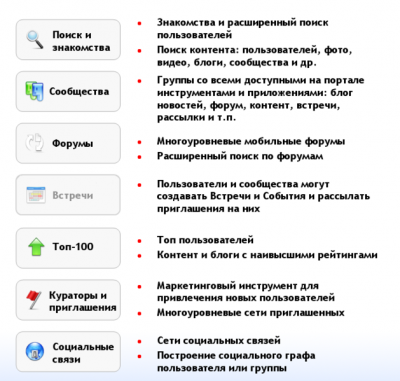
\includegraphics[scale=1]{sn-components.png} 
	\caption{Компоненты социальной сети}
	\label{fig:analysis:snComponents}
\end{figure}

Функции социальных сетей:
\begin{itemize}
	\item cоздание индивидуальных профилей, в которых будет содержаться определенная информация о пользователе;
	\item взаимодействие пользователей (посредством просмотра профилей друг друга, внутренней почты, комментариев и пр.);
	\item возможность достижения совместной цели путем кооперации (например, целью социальной сети может быть поиск новых друзей, ведение группового блога и пр.);
	\item обмен ресурсами (к примеру, ссылками на сайты);
	\item возможность удовлетворения потребностей за счет накопления ресурсов (например, путем участия в социальной сети можно обзаводиться новыми знакомыми и тем самым удовлетворять потребность в общении).
\end{itemize}

Классификация социальных сетей:
\begin{itemize}
	\item cоциальные сети в свободном доступе: не тематические сети и сугубо профессиональные сообщества практиков;
	\item cоциальные сети в корпоративном формате: cети в свободном доступе и не специализированные (сеть «общего профиля»).
\end{itemize}

Под не специализированными социальными сетями понимаются сообщества в интернете, не имеющие ограничений ни по каким параметрам и не имеющие никакой тематической специализации.

Специализированные социальные сети обычно являются платформой для сообществ специалистов. Они называются сообществами практиков (Community of Practice, CoP) и преследуют сугубо практические цели и объединяет людей, которые заинтересованы в приобретении и развитии знаний в определенной области, их использовании на практике. Сообщества практиков могут состоять из ученых, инженеров, специалистов по маркетингу и продажам и других специалистов. Причем эти сообщества не обязательно должны быть ограничены рамками одной компании, а могут объединять людей со схожими интересами в разных организациях по всему миру. CoP отличаются от сообществ по интересам — его участников объединяет не только стремление к некой области знаний, но и желание сотрудничать в процессе применения этих знаний на практике. Члены сообщества хорошо понимают друг друга, поскольку работают над схожими проблемами. Они способны оценить уровень квалификации, проблемы коллег, получить друг от друга недостающие им знания.

Социальные сети в корпоративном формате в первую очередь являются инструментом внутренних коммуникаций.
Т.к. темой дипломного проекта является создание тематической социальной сети -- разберем данный вид подробней.




\subsection{Тематические социальные сети}
\label{sec:analysis:analogues}

Социальная сеть - это отличный инструмент для общения, поддержки личных связей, обмена информацией. И когда-то социальные сети полностью подходили под это описание.
Сейчас все иначе, сейчас социальная сеть -- это медийный <<журнал>>, хаотичная смесь из информационно-развлекательного контента и рекламы. В основном пользователь не создает контент, он его потребляет в этом <<журнальном» формате>>. Приэтом существует огромное количество «рубрик» - групп по интересам, где можно найти информацию на любой вкус и цвет. В связи с этим личное общение уходит на второй план, и, с молчаливого согласия самого пользователя, он превращается в «подписчика». В отличие от того, какой контент ему интереснее, он выбирает Facebook или <<ВКонтакте>>, либо любую другую социальную сеть.

Вслед за сетями общего типа, стали развиваться \emph{тематические сети}, которые использовали тот же функционал, но в более ограниченной, конкретной нише. Сейчас этот процесс перешел в более активную стадию. Можно уже находить и регистрироваться в социальных сетях для туристов, спортсменов, меломанов, книголюбов, фотографов, ученых, политиков и т.д. Но, в мире так много таких ниш, что даже, казалось бы, популярные и то до сих пор не заполнены. 

Интересно, что практически все тематические сети -- это проекты глобального уровня, они не ориентированы только на одну определенную страну. Можно смело утверждать, что стадия, на которой создавались глобальные проекты, завершается. На смену ей идет стадия, на которой создаются тематические социальные сети на рынках локальных. И, как правило, зачастую они представляют собой клоны уже существующих популярных проектов. На смену количественному насыщению рынка тематическими проектами, идет развитие качественной стороны сетей. Таким образом, повторилась история развития общих сетей: на смену количественной пришла качественная составляющая конкуренции.

Современный пользователь вовсе не желает получать контент редакционный, который для него отобрали без учета его мнения. Он хочет не только сам этот процесс контролировать, но и участвовать в нем непосредственно, лично. Это и есть главная причина, по которой создают тематическую социальную сеть для каждой значимой тематики. Эти сети перетягивают на себя большинство пользователей из общего числа целевой аудитории. Такие сообщества основываются на взаимодействии между тематическим контентом и специфической коммуникацией пользователей. Причем значительное место в них отводится различным дополнительным сервисам (например, в области геолокации или электронной коммерции).





\subsection{Мобильная разработка}
Конечный успех программного проекта во многом определяется до начала конструирования: на этапе подготовки, которая проводится с учетом всех особенностей проекта.

Первое предварительное условие, которое нужно выполнить перед конструированием, -- ясное формулирование проблемы, которую система должна решать. Общая цель подготовки — снижение риска: адекватное планирование позволяет исключить главные аспекты риска на самых ранних стадиях работы, чтобы основную часть проекта можно было выполнить максимально эффективно. 

Главный факторы риска в создании ПО — неудачная выработка требований. Требования подробно описывают, что должна делать программная система. Внимание к требованиям помогает свести к минимуму изменения системы после начала разработки \cite{code_complete}.

Перед формулированием требований необходимо изучить ряд вопросов, которые напрямую влияют на все дальнейшие этапы разработки. В частности, необходимо рассмотреть вопросы выбора платформ, архитектуры. По результатам анализа можно будет составить техническое задание к проектируемому программному средству, которое станет основой для составления функциональных требований.

\subsubsection{} Обзор типов мобильной разработки
\label{sec:analysis:literature:platforms}

Разработка мобильных приложений, становится все более и более
востребованной, таким образом разработчики ищут новые возможности для
быстрой и качественной реализации проектов. Долгое время разработка
мобильных приложений являлась исключительно нативной, это обусловлено
достаточным качеством и быстродействием существующих IDE.

Таким образом, для того, что бы написать качественные программы для
двух наиболее распространенных платформ (Android, IOS) необходимо было
изучать такие языки программирования, как: Java, Kotlin, Swift~\cite{swift}, ObjectiveC~\cite{objectiveC}. Благодаря необходимости знания множества языков, компанией
Facebook был представлен фреймворк ReactNative~\cite{reactNaitve}, для написания на
котором требовалось знание JavaScript.

В ReactNative, в качестве ЯП используется
JavaScript, или несколько иной подход смешивающий синтаксис JavasScript и
HTML по типу JSX. Инструменты для ReactNative – это в основном текстовый
редактор, отладчик Chrome и несколько других инструментов для сборки и
тестирования. 

Для нативной разработки IOS необходимо знание языка Swift или
Objective-C, а для Android – Java или Kotlin. Инструменты для создания
приложения находятся в IDE каждой платформы: для IOS это X-code, а для
Android это Android studio. Так же для программирования в каждой из этих IDE,
необходимо знать как работать в этой среде, как работают системы отладки и
сборки.

ReactNative берет свое начало в веб-разработке и заимствует свою
базовую части именно оттуда, в то время как для нативной разработки такой
базовой части не существует. Это исключительно нативные сенсорные
платформы, которые необходимо изучать. Так же стоит отметить, что когда
изучена одна из IDE, вторая изучается достаточно быстро.

Фреймворки являются очень значимым показателем выбора в сторону
нативной разработки. Необходимо изучить как работают все интересующие вас
функции, но в отличии от ReactNative, все эти функции задокументированы и
реализованы. 

\begin{figure}[H]
	\centering
	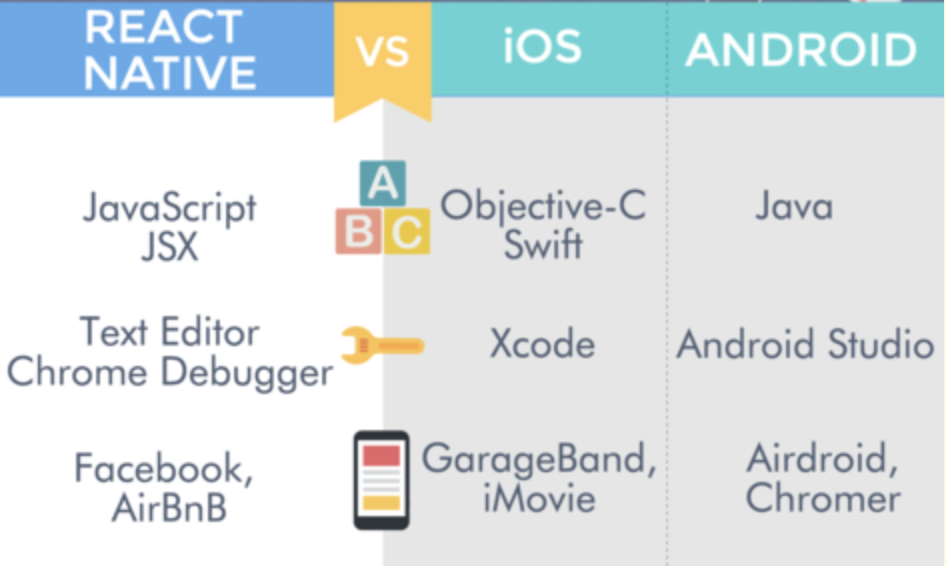
\includegraphics[scale=1]{rn-vs-androi-vsios.png} 
	\caption{Сравнение нативной и кроссплатформенной разработки}
	\label{fig:analysis:analogues:bsuir}
\end{figure}

Swift и ReactNative совсем недавно появились в программировании, при
этом каждый из них отлично документирован. Официальная документация
apple, позволяет разобраться во всех тонкостях нового языка, с примерами
применения и полезными советами начинающим разработчикам. В то же время 
официальная документация Facebook по ReactNative, тоже раскрывает все
возможности фреймворка, с примерами кода и типовой документацией. 

\subsubsection{} Обзор архитектурных стилей
\label{sec:analysis:literature:architecture}

Существует множество различных архитектурных шаблонов для
разработки мобильных IOS приложений. Выбор архитектуры будущего
приложения очень важный этап проектирования. Правильный выбор
архитектуры, позволит проводить поиск ошибок, а так же оперативно
реагировать на изменения внутри класса. 

В настоящее время есть множество вариантов шаблонов проектирования
архитектуры, среди них выделяются следующие: MVC, MVP, VIPER.
MVC, MVP, MVVM предполагают включение объектов приложения в
одну из трех категорий: 
\begin{itemize}
	\item Models -- ответственные за данные домена или уровень доступа к
	данным, который манипулирует данными;
	\item Views -- ответственны за уровень представления, все элементы с префиксом UI;
	\item Controller, Presenter, ViewModel -- выполняет роль посредника
	между Model и View, отвечающего за изменения Model и реагируя на действия
	пользователя, выполняемые во View и обновляя View с изменениями из Model.
\end{itemize}

Далее подробнее рассмотрим каждый из представленных выше
шаблонов.

При использовании шаблона традиционного MVC, View не имеет
состояния, он просто отображается контроллером после изменения модели~\cite{mvc}.
Таким образом, этот шаблон подразумевает полную перезагрузку страницы
после любого действия пользователя.

Таким образом, реализация традиционного MVC в приложении IOS не
имеет смысла из-за архитектурной проблемы – все три объекта связаны друг с
другом и каждая сущность знает о двух других (рисунок~\ref{fig:analysis:tradMvc}).

\begin{figure}[H]
	\centering
	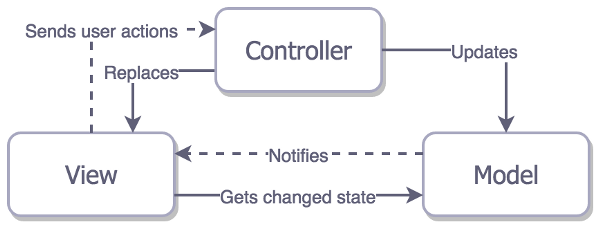
\includegraphics[scale=0.55]{traditionalMVC.png} 
	\caption{Традиционный MVC}
	\label{fig:analysis:tradMvc}
\end{figure}

В шаблоне архитектуры Apple MVC (рисунок~\ref{fig:analysis:appleMVC}) контроллер будет являться
посредником между View и Model, что бы эти два объекта не знали о
существовании друг друга~\cite{mvcApple}. Наиболее часто используемым объектом будет
являться контроллер. В этом есть плюсы, потому что в приложении должно
быть место для всей сложной бизнес-логики, которая не вписывается в Model. 

\begin{figure}[H]
	\centering
	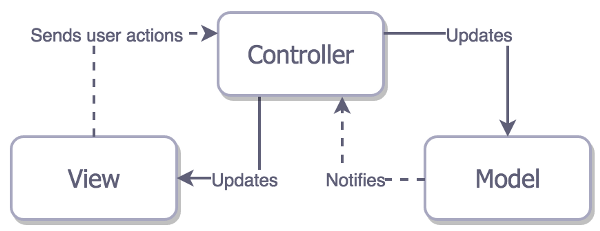
\includegraphics[scale=0.55]{appleMVC.png} 
	\caption{Apple MVC}
	\label{fig:analysis:appleMVC}
\end{figure}

В реальности шаблон Apple MVC работает по-другому.
Перегруженный контроллер содержит в себе большое количество бизнеслогики, превращая Model-View-Controller в Massive-View-Controller. Cocoa
MVC поощряет писать Massive-View-Controller, потому что они вовлечены в жизненный цикл View, что приводит к неразделимости
этих двух сущностей (рисунок~\ref{fig:analysis:realAppleMVC}). 

\begin{figure}[H]
	\centering
	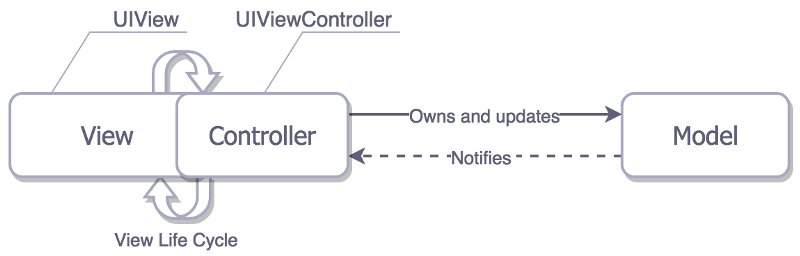
\includegraphics[scale=0.55]{realAppleMVC.png} 
	\caption{Практический Apple MVC}
	\label{fig:analysis:realAppleMVC}
\end{figure}

MVP (Cocoa MVC’s promises delivered) похож на Apple MVC, но это не
так[16]. В Apple MVC – View связан с контроллером, в то время как медиатор
MVP – Presenter, не имеет ничего общего с жизненным циклом контроллера,
поэтому в Presenter нет кода для установки макета экрана, но он отвечает за
обновление View с актуальными данными и состоянием. 

MVP это архитектурный шаблон, показывающий проблемы сборки,
которая возникает из-за наличия трех фактически разделенных слоев (рисунок~\ref{fig:analysis:mvpPic}).

\begin{figure}[H]
	\centering
	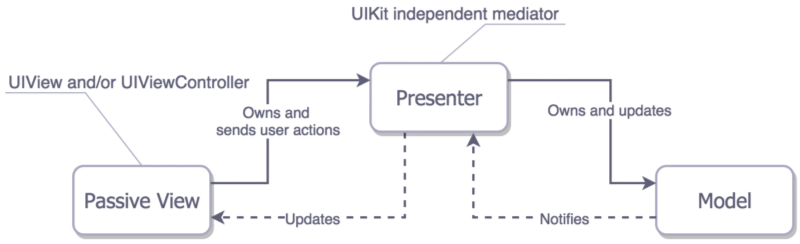
\includegraphics[scale=0.55]{mvp.png} 
	\caption{MVP}
	\label{fig:analysis:mvpPic}
\end{figure}

Существует и другой формат MVP – MVP Supervising Controller~\cite{mvcAppleReal}.
Этот вариант включает прямую зависимость View и Model, в то время как
Presenter (Supervising Controller) все еще обрабатывает действия из View и
способен его изменять. Разделение смутной ответственности, является
недопустимым, так же как и сильная связь View и Model (рисунок~\ref{fig:analysis:MvPbh}). 

\begin{figure}[H]
	\centering
	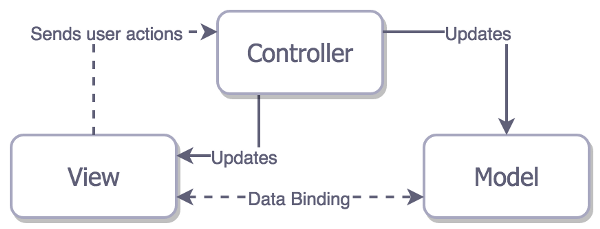
\includegraphics[scale=0.55]{MvPbh.png} 
	\caption{MVP (Bindings and Hooters)}
	\label{fig:analysis:MvPbh}
\end{figure}

MVVM рассматривает контроллер View, как View, а так же
подразумевает отсутствие связи между View и Model~\cite{mvvmApple}. View-Model
обеспечивает независимое представление View и его состояния. View-Model
вызывает изменения в Model и обновляет себя с обновленной Model, а
поскольку View и View-Model соединены, View соответственно тоже
обновляется (рисунок~\ref{fig:analysis:mvvm}). 

\begin{figure}[H]
	\centering
	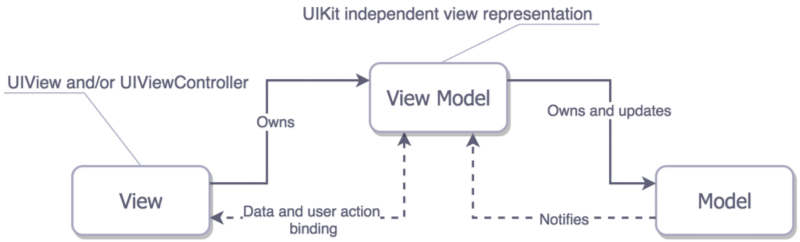
\includegraphics[scale=0.55]{mvvm.png} 
	\caption{MVVM}
	\label{fig:analysis:mvvm}
\end{figure}

VIPER позволяет полностью разделить обязанности, и обеспечить
полную независимость модулей~\cite{viper}. Он состоит из: 
\begin{itemize}
	\item View – отвечающее за исполнение произошедших в Presenter
	изменений;
	\item Presenter – содержит связанную с UI (независимую от UIKit)
	бизнес-логику, вызывает методы в Interactor;
	\item Entities – в этом классе хранятся простые объекты данных;
	\item Interactor – содержит бизнес-логику, связанную с данными
	(Entities) или сетевыми устройствами. В его обязанности входят такие
	операции, как создание новых экземпляров объектов, или выборку их с сервера.
	Для этих целей используются службы и менеджеры, не являющиеся частью
	модуля VIPER – они являются внешней зависимостью (рисунок~\ref{fig:analysis:viper}).
\end{itemize}

\begin{figure}[H]
	\centering
	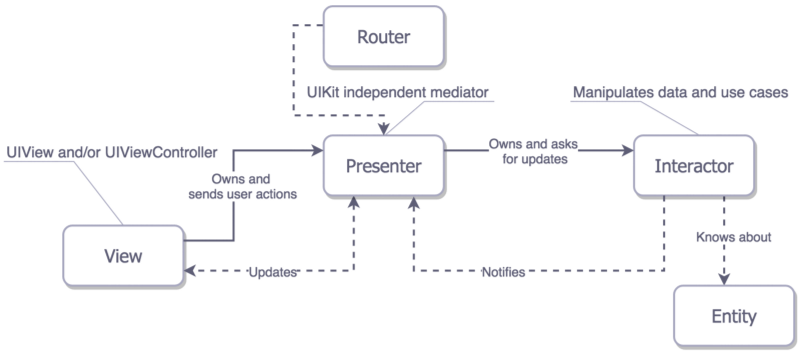
\includegraphics[scale=0.55]{viper.png} 
	\caption{VIPER}
	\label{fig:analysis:viper}
\end{figure}

Модуль VIPER может соответствовать как одному экрану в
приложении, так и всему приложению, четких указаний как выбрать размер
модуля не приводится.
VIPER – это первый шаблон в котором явно рассматривается
навигационная ответственность, которая решается при помощи Router.

% \subsubsection{} Проектирование баз данных
% \label{sec:analysis:literature:db}

% В настоящее время сложно представить сложные приложения, которые бы не использовали специальные средства для хранения информации.

% База данных -- представленная в объективной форме совокупность самостоятельных материалов, систематизированных таким образом, чтобы эти материалы могли быть найдены и обработаны с помощью ЭВМ. Модель базы данных -- описание базы данных с помощью  определенного (в т.ч. графического) языка на некотором уровне абстракции.




\subsection{Кроссплатформенность приложений} 
\label{sec:analysis:literature:crossplatform}

Как несколько десятилетий назад, так и в настоящее время выбор платформы является серьезным ограничением для всех последующих этапов разработки. Однако уже начали появляться технологии, которые позволяют использовать однажды написанный код на многих платформах. Сегодня все больше приложений создается сразу для нескольких платформ, а приложения, созданные изначально для одной платформы, активно адаптируются под другие \cite{crossplatform}. В случае мобильных приложений, код такого приложения работает как под IOS, так и под Android платформы. Разработчик, изучающий какую-либо из таких технологий, получает конкурентное преимущество, поскольку за счет расширения количества платформ расширяется круг задач, над которыми он может работать. Поэтому кроссплатформенность -- реальная или потенциальная -- является одним из факторов, который необходимо учитывать при выборе технологий реализации проекта.


\subsection{Требования к проектируемому программному средству}
\label{sec:analysis:specification}

По результатам изучения предметной области, анализа литературных источников и обзора существующих систем-аналогов сформулируем требования к проектируемому программному средству.

\subsubsection{} Назначение проекта
\label{sec:analysis:specification:purpose}

Назначением проекта является разработка программного средства, представляющего специализированную (тематическую) социальную сеть для мотоциклистов.

\subsubsection{} Основные функции
\label{sec:analysis:specification:functions}

Программное средство должно поддерживать следующие основные фун\-к\-ции:

\begin{itemize}
	\item регистрация и аутентификация;
	\item управление друзьями и подписчиками;
	\item отправка сообщений;
	\item просмотр профиля пользователя;
	\item возможность создания и поиска публикаций, содержащих текст, фото и видеоматериалы;
	\item возможность добавления хештегов к описаниям публикаций;
	\item ведение личного блога;
	\item прикрепления информации о мотопарке пользователя к его профилю;
	\item установка статуса, уведомляющего о передвижение на мотоцикле в данными момент времени;
	\item просмотр карты с геолокацией,
	\item установка на карте меток предупрежения;
	\item подача сигнала <<SOS>>;
	\item отправка сигнала, представляющего собой запрос на совместную поездку (маячок); 
	\item отправка push-уведомлений.
\end{itemize}

\subsubsection{} Выбор технологий программирования
\label{sec:analysis:specification:language}

На данный момент на рынке мобильных устройств выделяются 2 основные платформы (операционные системы): Android и IOS. Разрабатываемое мобильное приложение должно работать на обеих платформах, при этом стоит цель минимизировать время разработки продукта без потерь его качества. До недавнего времени приходилось разрабатывать 2 отдельных приложения, копируя до 90 \% общего кода. Однако всё больше внимания привлекают кроссплатформенные решения, которые базируются на применении кроссплатформенных сред разработки.

При проведении анализа рынка возможностей разработки мобильных приложений, был выбран данный подход с использованием React-Native.
Для вхождения в разработку с помощью React-Native, нет необходимости осваивать новые языки, если JavaScript, HTML, CSS уже изучены, а программирование напоминает
создание веб интерфейса для веб версий. Инструменты и архитектура приложения такие же, как и при в веб-разработке. 

После анализа возможных архитекрутрных решение (\ref{sec:analysis:literature:architecture}) было приянято решение использовать шаблон проектирования Viper.

Viper превосходит все представленные архитектурные паттерны в
распределённой, тестируемости, и простоте освоения новых модулей.
Основными особенностями Viper является распространение – VIPER
отличается отличной способностью к распределению обязанностей,
тестируемость – при лучшем распределении, получается лучшая тестируемость.
Так же удобство использования – маленькое количество кода в блоках VIPER,
позволяет без труда переключаться с одной задачи на другую, увеличивая тем
самым полезную работу программиста.
Можно сделать вывод, что для наилучшего распределения обязанностей,
и покрытия приложения тестами приложения, больше всего подходит
архитектурный шаблон -- Viper. 

Сформулированные требования позволят осуществить успешное проек- тирование и разработку программного средства.




	\section{Проектирование кроссплатформенного мобильного приложения для социальной сети мотоциклистов}
\label{sec:domain}

Функциональная модель программного средства представлена в виде\linebreakсхемы алгоритма процесса обучения и диаграммы вариантов использования и информационной модели предметной области. Варианты использования отражают функциональность системы в ответ на внешние воздействия с точки зрения получения значимого результата для пользователей. Информационная модель предметной области в дальнейшем будет использоваться при проектировании базы данных для программного средства.

\subsection{Анализ процесса организации совместной мотоциклистов} 
\label{sec:domain:model:deeds}

BPMN (нотация моделирования бизнес-процессов) --- это графический язык для выражения концепций, связанных с BPM, с использованием методов потоковой диаграммы.
Его нотация легко читаема и понятна для конечных пользователей и всех других технических специалистов, участвующих в определении проекта BPM. Процессы могут визуально описываться пользователями и реализовываться техническими специалистами, преодолевая существующий разрыв между ними. В этом смысле BPMN является точкой связи внутри организации между нетехническим персоналом и ИТ-отделом~\cite{bpmn}.

\begin{figure}[H]
	\centering
		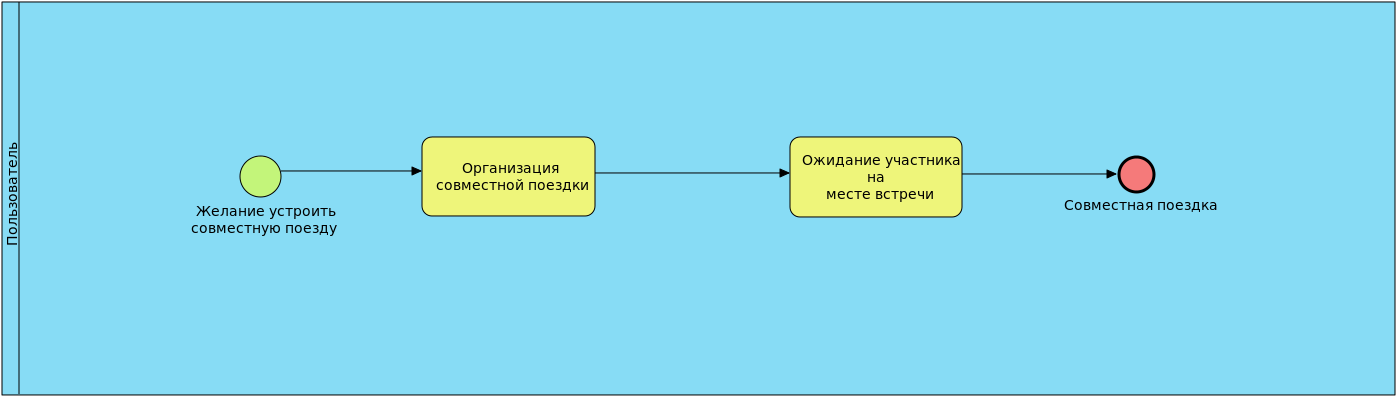
\includegraphics[scale=0.32]{2process-1.png}
		\caption{BPMN диаграмма процесса организации совместной поездки}
		\label{fig:domain:model:1}
	\end{figure}

Разберем задачу организации совместной поездки подробней (рисунок~\ref{fig:domain:model:2}). 

\begin{figure}[H]
	%\ContinuedFloat
	\centering
		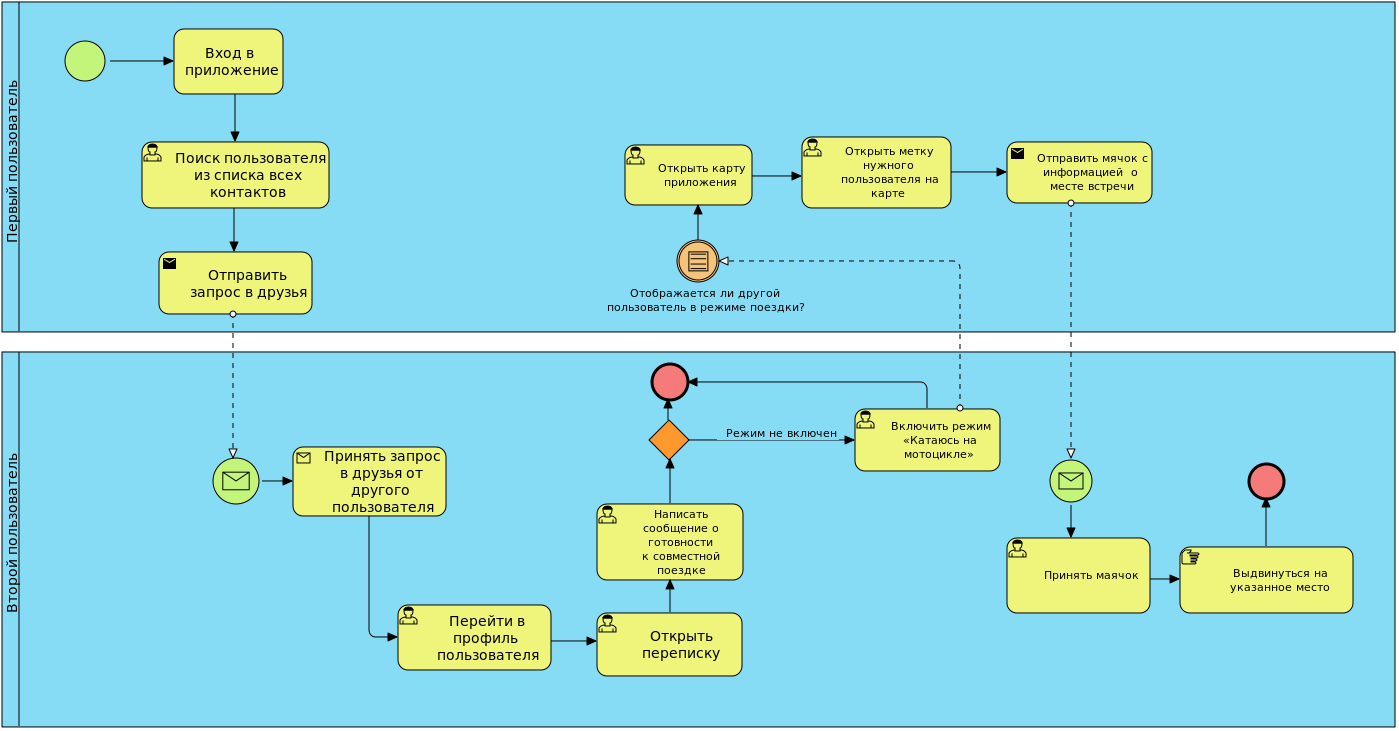
\includegraphics[scale=0.32]{2process-2.png}
		\caption{Расширение BPMN для задачи организации совместной поездки}
		\label{fig:domain:model:2}
	\end{figure}

	Таким образом с помощью диаграммы BPMN приведен типичный вариант организации совместной поездки мотоциклистов

\subsection{Варианты использования программного средства}
\label{sec:domain:model:use_cases}

В результат анализа предметной области и существующих аналогов можно сделать вывод, что проектируемое программное средство должно поддерживать набор функций, который бы полностью удовлетворял потребности пользователей с точки зрения обычной социальной сети, а также специфические функции, необходимые только для мотоцикслистов. Выделим следующие:

\begin{itemize}
	\item \emph{Интеграция с существуюшими социальными сетями}, которая позволит производить авторизацию в приложении с использованием существующих учетных записей пользователей из других социальных сетей.
	\item \emph{Сообщения} позволяют обмениваться информацией, находить друзей и единомышленников.
	\item \emph{Публикации} представляют собой записи, которые могут содержать фото, видеофайлы и текст записи с хештегами.
	\item \emph{Управления мотопарком}. Возможность прикрепления информации о мотопарке пользователя: создание публикаций с указанием технических характеристик мотоциклов, а также удаление и редактирование данной информации.
	\item \emph{Гараж}. Страница отображает информацию о мотопарке пользователя: фотографии, видео, технические характеристики, комментарии других пользователей, лайки. 
	\item \emph{Профиль пользователя}. Отдельная страница, которая отображает краткую информацию о человеке, его мотопарке, а также содержит секцию с публикациями пользователя.
	\item \emph{Личный блог}. Возможность ведения личного блога предусматривает создание публикаций с пометкой <<Запись>>. Данные публикации будут отмечены специальным индефикатором в секции со всеми публикациями (профиль пользователя).
	\item \emph{Управление друзьями и подписчиками}. Возможность отправки и отмены запросов на добавления в друзья, поиск других пользователей.
	\item \emph{Отправка оповещений}. Возможность отправки оповещений о состоянии приложения, а также о действиях других пользователей (комментирование публикакации, добавление лайков на запись).
	\item \emph{Настройка учетной записи} позволит изменять информацию о пользователе, прикреплять ссылки на другие социальные сети, устанавливать настройки приватности, изменять пароль.
	\item \emph{Лента}. Отдельная страница, которая представляет собой список публикаций. Следует предусмотреть ее разграничение на публикации, размещенные только друзьями, и на популярные, которые получили больше всего лайков в приложении.
	\item \emph{Режим катания на мотоцикле}. Возможность переключения в данный режим указывет на то, что пользователь в данный момент едет на мотоцикле или изъявляет желание покататься.
	\item \emph{Карта}. Отдельный раздел приложения, который представляет собой страницу, содержащую карту с геолокацией, на которой отмечены друзья, у которых установлен режим катания на мотоцикле, а также метки. Следует предусмотреть функцию возврата фокуса к текущему местоположению, а также поиск друзей.
	\item \emph{Метки}. Специальные маркеры на карте, которые будут служить инструментом предупреждения других пользователей об опаснастях и чрезвычайных ситуациях на дороге.
	\item \emph{Маячок}. Возможность отправки специального сигнала в виде текстового сообщения другу, который в данный момент катается на мотоцикле, т.е. отмечен на карте.
	%которые отображаются на карте, бывают двух типов: <<Предупреждение>> и <<SOS>>. При установке последнего пользователем его друзьям должно приходить оповещение с оповещение должно приходить 
\end{itemize}

Диаграмма вариантов использования представлена на рисунке~\ref{fig:domain:model:use_cases:model}.
Рассмотрим некоторые из представленных на рисунке прецедентов.

\begin{figure}[H]
\centering
	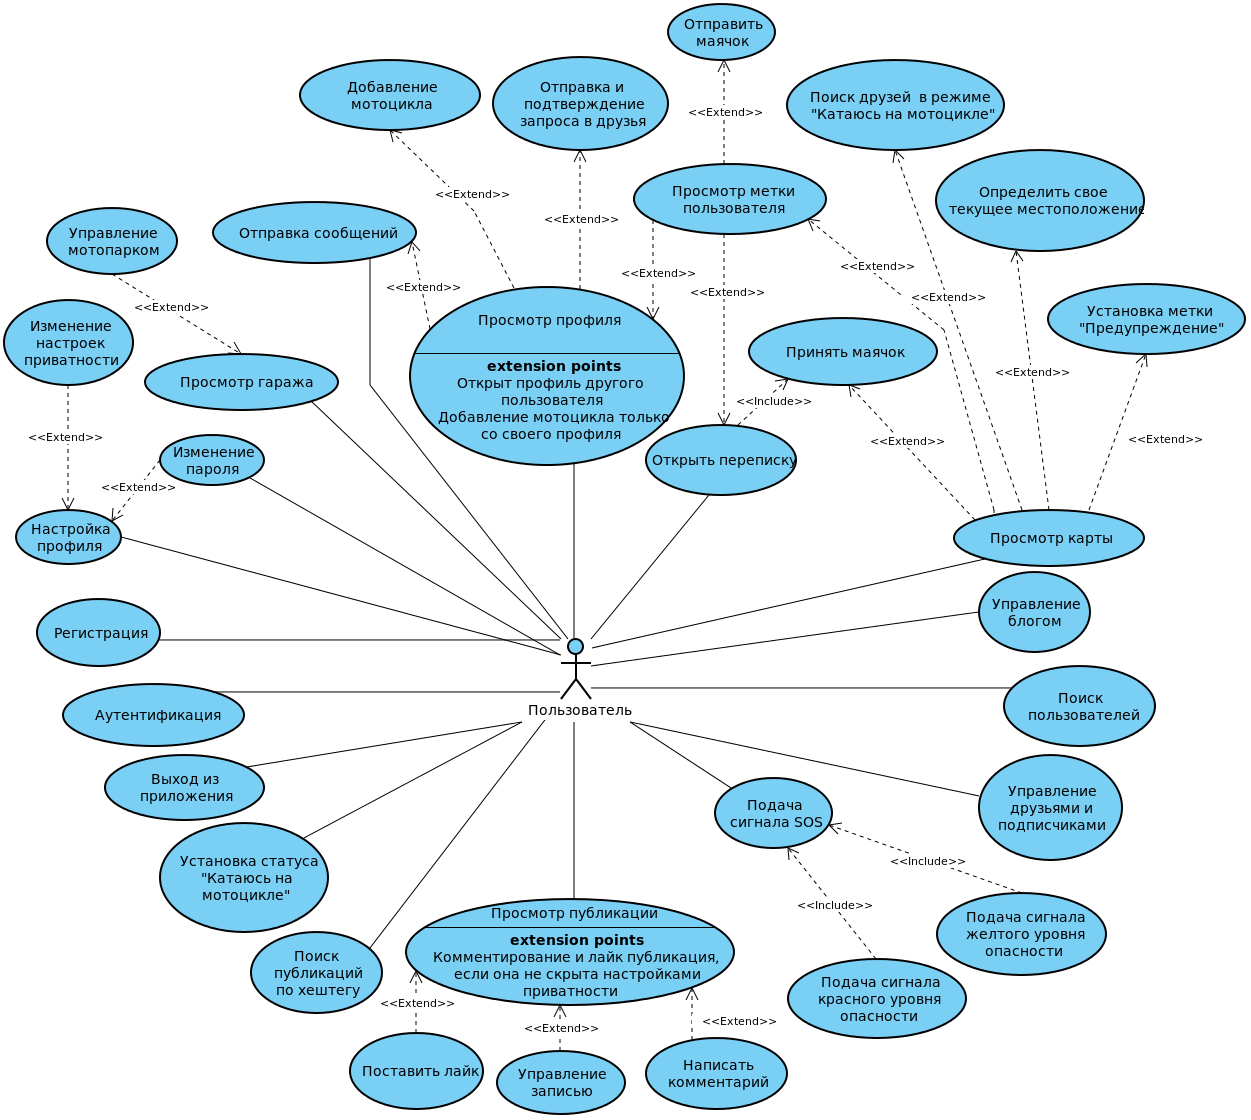
\includegraphics[height=230mm, width=155mm]{use-case-diagram.png}
	\caption{Диаграмма вариантов использования ПС}
	\label{fig:domain:model:use_cases:model}
\end{figure}

\emph{Регистрация, аутентификация и авторизация}. В приложения планируется реализация собственной системы авторизации, а также возможность регистрации с помощью учетных записей от других социальных сетей (\facebook~и \vk.).
Важно предусмотреть возможность редактирование информации о пользователе, в том числе и его учетных данных (н.п. \emph{смена пароля}). Для этих целей будет создан специальный раздел с \emph{настройками профиля}.
Также следует предусмотреть возможность смены пароля со страницы входа в приложение, т.к. пользователь может забыть пароль.
Важной функцией приложения станет \emph{изменение настроек приватности}, что даст возможность ограничить видимость информации о себе и публикакаций от других пользователей. 

\subsection{Разработка спецификации функциональных требований}
\label{sec:domain:specification}

С учетом требований, определенных в подразделе \ref{sec:analysis:specification}, представим детализацию функций проектируемого ПС.

\subsubsection{} Функция регистрации
\label{sec:domain:specification:signup}

Функция регистрации должна быть реализована с учетом следующих требований:
\begin{itemize}
	\item для регистрации пользователь обязан предоставить номер мобильного телефона и пароль;
	\item возможность альтернативной регистрации с помощью социальных сетей <<ВКонтакте>> и Facebook;
	\item проверка номера мобильного телефона проверяется отправкой SMS-сообщения с кодом подверждения;
	\item хранение пароля в хешированном виде; алгоритм шифрования должен превосходить или быть равным семейству SHA-2. Использование соли обязательно;
	\item предусмотреть возможность смены пароля после регистрации путем отправки SMS-сообщение с кодом, ввод которого перенаправляет на страницу изменения пароля.
\end{itemize}

\subsubsection{} Функция аутентификации
\label{sec:domain:specification:authentication}

Функция аутентификации должна быть реализована с учетом следующих требований:
\begin{itemize}
	\item инициатором является пользователь, при этом необходимо предоставить номер мобильного телефона и пароль, либо выбрать вход через Facebook или <<ВКонтакте>>;
	\item должна быть реализована возможность повторной аутентификации пользователя без необходимости ввода какой-либо информации;
	\item возможность восстановления пароля.
\end{itemize}

Для восстановления пароля пользователь должен предоставить номер мобильного телефона. На предоставленный номер высылается SMS-сообщение с кодом подверждения. После ввода отправленного кода ему предоставляется возможность установить новый пароль.

\subsubsection{} Функция управления публикациями
\label{sec:domain:specification:agenda}

Публикации являются главной единицой обмена информацией в социальной сети. При реализации данной функции необходимо учесть следующие требования:
\begin{itemize}
	\item необходимо обеспечить возможность добавления, удаления, редактирования публикации;
	\item публикация может включать в себя текст, фото или видео;
	\item для ведения личного блога создать отдельный раздел <<Записи>>; все публикации, созданные в данном разделе, будут относится к блогу пользователя;
	\item записи с личного блога должны быть помечены специальным идентификатором в галлерее публикаций профиля пользователя;
	\item должна быть реализована возможность загрузки фото и видео как с галерии мобильного телефона, так и с его камеры;
	\item предусмотреть возможность указания хештегов в тексте, что облегчит поиск нужных публикаций в ленте;
	\item добавить возможность наложения цветовых фильтров на фотографии, как в социальной сети Instagram;
	\item предусмотреть возможность комментирования и лайка публикации с отображением количества лайков и всей истории комментариев;
	\item при нажатии на количество лайков появляется список всех лайкнувших пользователей через который можно перейти к ним в профиль.
	\item при нажатии на публикацию она должна открываться на отдельной странице (галлерия профиля, гараж, лента).
\end{itemize}

\subsubsection{} Функция управления мотопарком
\label{sec:domain:specification:subjects}

Функция управления мотопарком должна быть реализована с учетом следующих требований:
\begin{itemize}
	\item мотоцикл представляет собой обычную публикацию с дополнительной возможностью прикрепления нескольких фото и видеозаписей. Описание публикации в данном случае --- характеристики мотоцикла;
	\item характеристики мотоцикла представить следующими полями: производитель, модель, прозвище, модификация, год, цвет, пробег, объем двигателя, мощность, описание;
	\item предоставить возможность добавления, редактирования, измения записей о мотоциклах;
	\item все добавленные мотоциклы формирует страницу <<Гараж>>, которая представляет собой список всех прикрепленных мототоциклов.
\end{itemize}

\subsubsection{} Функция обмена сообщениями
\label{sec:domain:specification:messages}

Функция коммуникации должна реализовывать следующие требования:
\begin{itemize}
	\item должна быть возможность отправки сообщений одного пользователя другому;
	\item история сообщений представляется в виде диалогов, где отображается текст сообщения, имя пользователя и время отправки сообщения;
	\item возможность прикрепления фотографии к сообщению (с галерии или с камеры телефона);
	\item предоставить возможность удаления выбранного диалога, а также поиска нужного.
\end{itemize}

\subsubsection{} Функция просмотра профиля пользователя
\label{sec:domain:specification:student_history}

Следующая группа требований относится к профилю пользователя:
\begin{itemize}
	\item профиль пользователя состоит из следующих секциий: аватар, информация о пользователе (количество мотосезонов и т.д.) и мотоциклах, количество друзей, подписчиков, подписок, записей, галлерея публикаций;
	\item предоставить возможность добавления новой публикации и прикрепления мотоцикла со страницы профиля;
	\item должна быть возможность отправки запроса в друзья при переходе в профиль другого пользователя;
	\item при переходе в профиль друга добавить возможность  перенаправления на страницу с диалогом;
\end{itemize}

\subsubsection{} Функция просмотра ленты
\label{sec:domain:specification:student_history}

Функция просмотра ленты должна реализовывать следующие требования:
\begin{itemize}
	\item лента представляет собой отдельную страницу со списком публикаций и полем поиска;
	\item поиск осуществляется по хештегам, указанным в тексте описания публикации;
	\item предоставить возможность разделения списка публикаций на 2 вида: принадлежащие друзьям и популярные (по количеству лайков).
\end{itemize}

\subsubsection{} Функция просмотра ленты
\label{sec:domain:specification:student_history}

Функция просмотра ленты должна реализовывать следующие требования:
\begin{itemize}
	\item лента представляет собой отдельную страницу со списком публикаций и полем поиска;
	\item поиск осуществляется по хештегам, указанным в тексте описания публикации;
	\item предоставить возможность разделения списка публикаций на 2 вида: принадлежащие друзьям и популярные (по количеству лайков).
\end{itemize}

\subsubsection{} Функция подачи сигнала SOS
\label{sec:domain:specification:student_history}

Следующая группа требований относится к установке сигнала SOS:
\begin{itemize}
	\item создать отдельный раздел в навигации приложения для установки сигнала;
	\item сигнал SOS должен отображаться в виде метки на карте;
	
	\item метка SOS устанавливается только в случае ДТП;
	
	\item сигнал должен иметь разделение на уровень тревоги: красный и желтый;
	\item красный сигнал подается только при опасности для здоровья;
	\item каждая метка, которая отображает сигнал, должна быть окрашена в соответствующий уровню тревоги цвет;
	\item при отправке пользователем сигнала красного уровня всем его друзья должно приходить push-уведомление.
\end{itemize}

\subsubsection{} Функция просмотра карты
\label{sec:domain:specification:student_history}

Функция просмотра карты должна реализовывать следующие требования:
\begin{itemize}
	\item карта представляет собой раздел геолокации, на котором отображаются метки следующих типов: друзья в режиме <<Катаюсь на мотоцикле>> (отображается в виде аватара), метки предупреждений и сигналов SOS;
	\item при нажатии на метку предупреждения или сигнала SOS на карте должно появляться ее текстовое описание;
	\item при установке метки предупреждения обязательно нужно указать ее текстовое описание;
	\item предусмотреть возможность опредения своего текущего местоположения;
	\item добавить отдельную кнопку для уставноки метки предупреждения;
	\item предусмотреть возможность поиска друзей, которые катаются на мотоцикле в данный момент врмени.
\end{itemize}

\subsubsection{} Функция отправки маячка
\label{sec:domain:specification:student_history}

Функция отправки маячка должна реализовывать следующие требования:
\begin{itemize}
	\item для отправки маячка следует перейти в карту приложения и выбрать нужного пользователя;
	\item по нажатию на метку пользователя должно появляться всплывающее окно, содержащее поле ввода маячка, а также кнопки перехода в диалог и профиль;
	\item адресату маячка должно приходить push-уведомление на телефон, а также сообщение в диалог с отправителем;
	\item принять маячок можно перейдя в диалог с отправителем, нажав кнопку <<Принять маячок>>;
	\item если у адресата в момент отправления откыта карта, то должно появляться всплывающее окно, в котором также можно его принять;
\end{itemize}

\subsubsection{} Функция управления друзьями и подписчиками
\label{sec:domain:specification:student_history}

Функция управления друзьями и подписчиками должна реализовывать следующие требования:
\begin{itemize}
	\item предусмотреть создание отдельного раздела <<Друзья>>, который разделен на 3 секции: друзья, запросы, подписки;
	\item секция состоит из списка соответсвующих пользоватателей и 2-ух счетчиков: первый отображает общее количество, а 2-ой количество находящихся в сети;
	\item релизовать возможности отправки и принятия запроса в друзья, а также удаление из друзей;
	\item при отправке запроса дружбы пользователю также отправляется соответсвующее push-уведомление.
	\item для подписки на другого пользователя достаточно отправить запрос в друзья, при этом данный пользователь будет отображен в секции подписок;
	\item запросы в дружбу, отправленные пользователю, можно посмотреть в секции запросов;
	\item если один пользователь удаляет другого, то у первого второй переносится в подписчики, а у второго первый в подписки соответственно;
	\item первый пользователь может вернуть второго в друзья перейдя в секцию запросов.
\end{itemize}

\subsection{Инфологическая модель базы данных}
\label{sec:domain:model:db}

Исходя из необходимости использования в проектируемом приложении базы данных, разработаем ее инфологическую модель. Диаграмма, представляющая модель базы данных инфологического уровня~\cite{kulikov_db_workbook}, представлена на рисунке~\ref{fig:domain:model:db:model}.

\begin{figure}[H]
\centering
	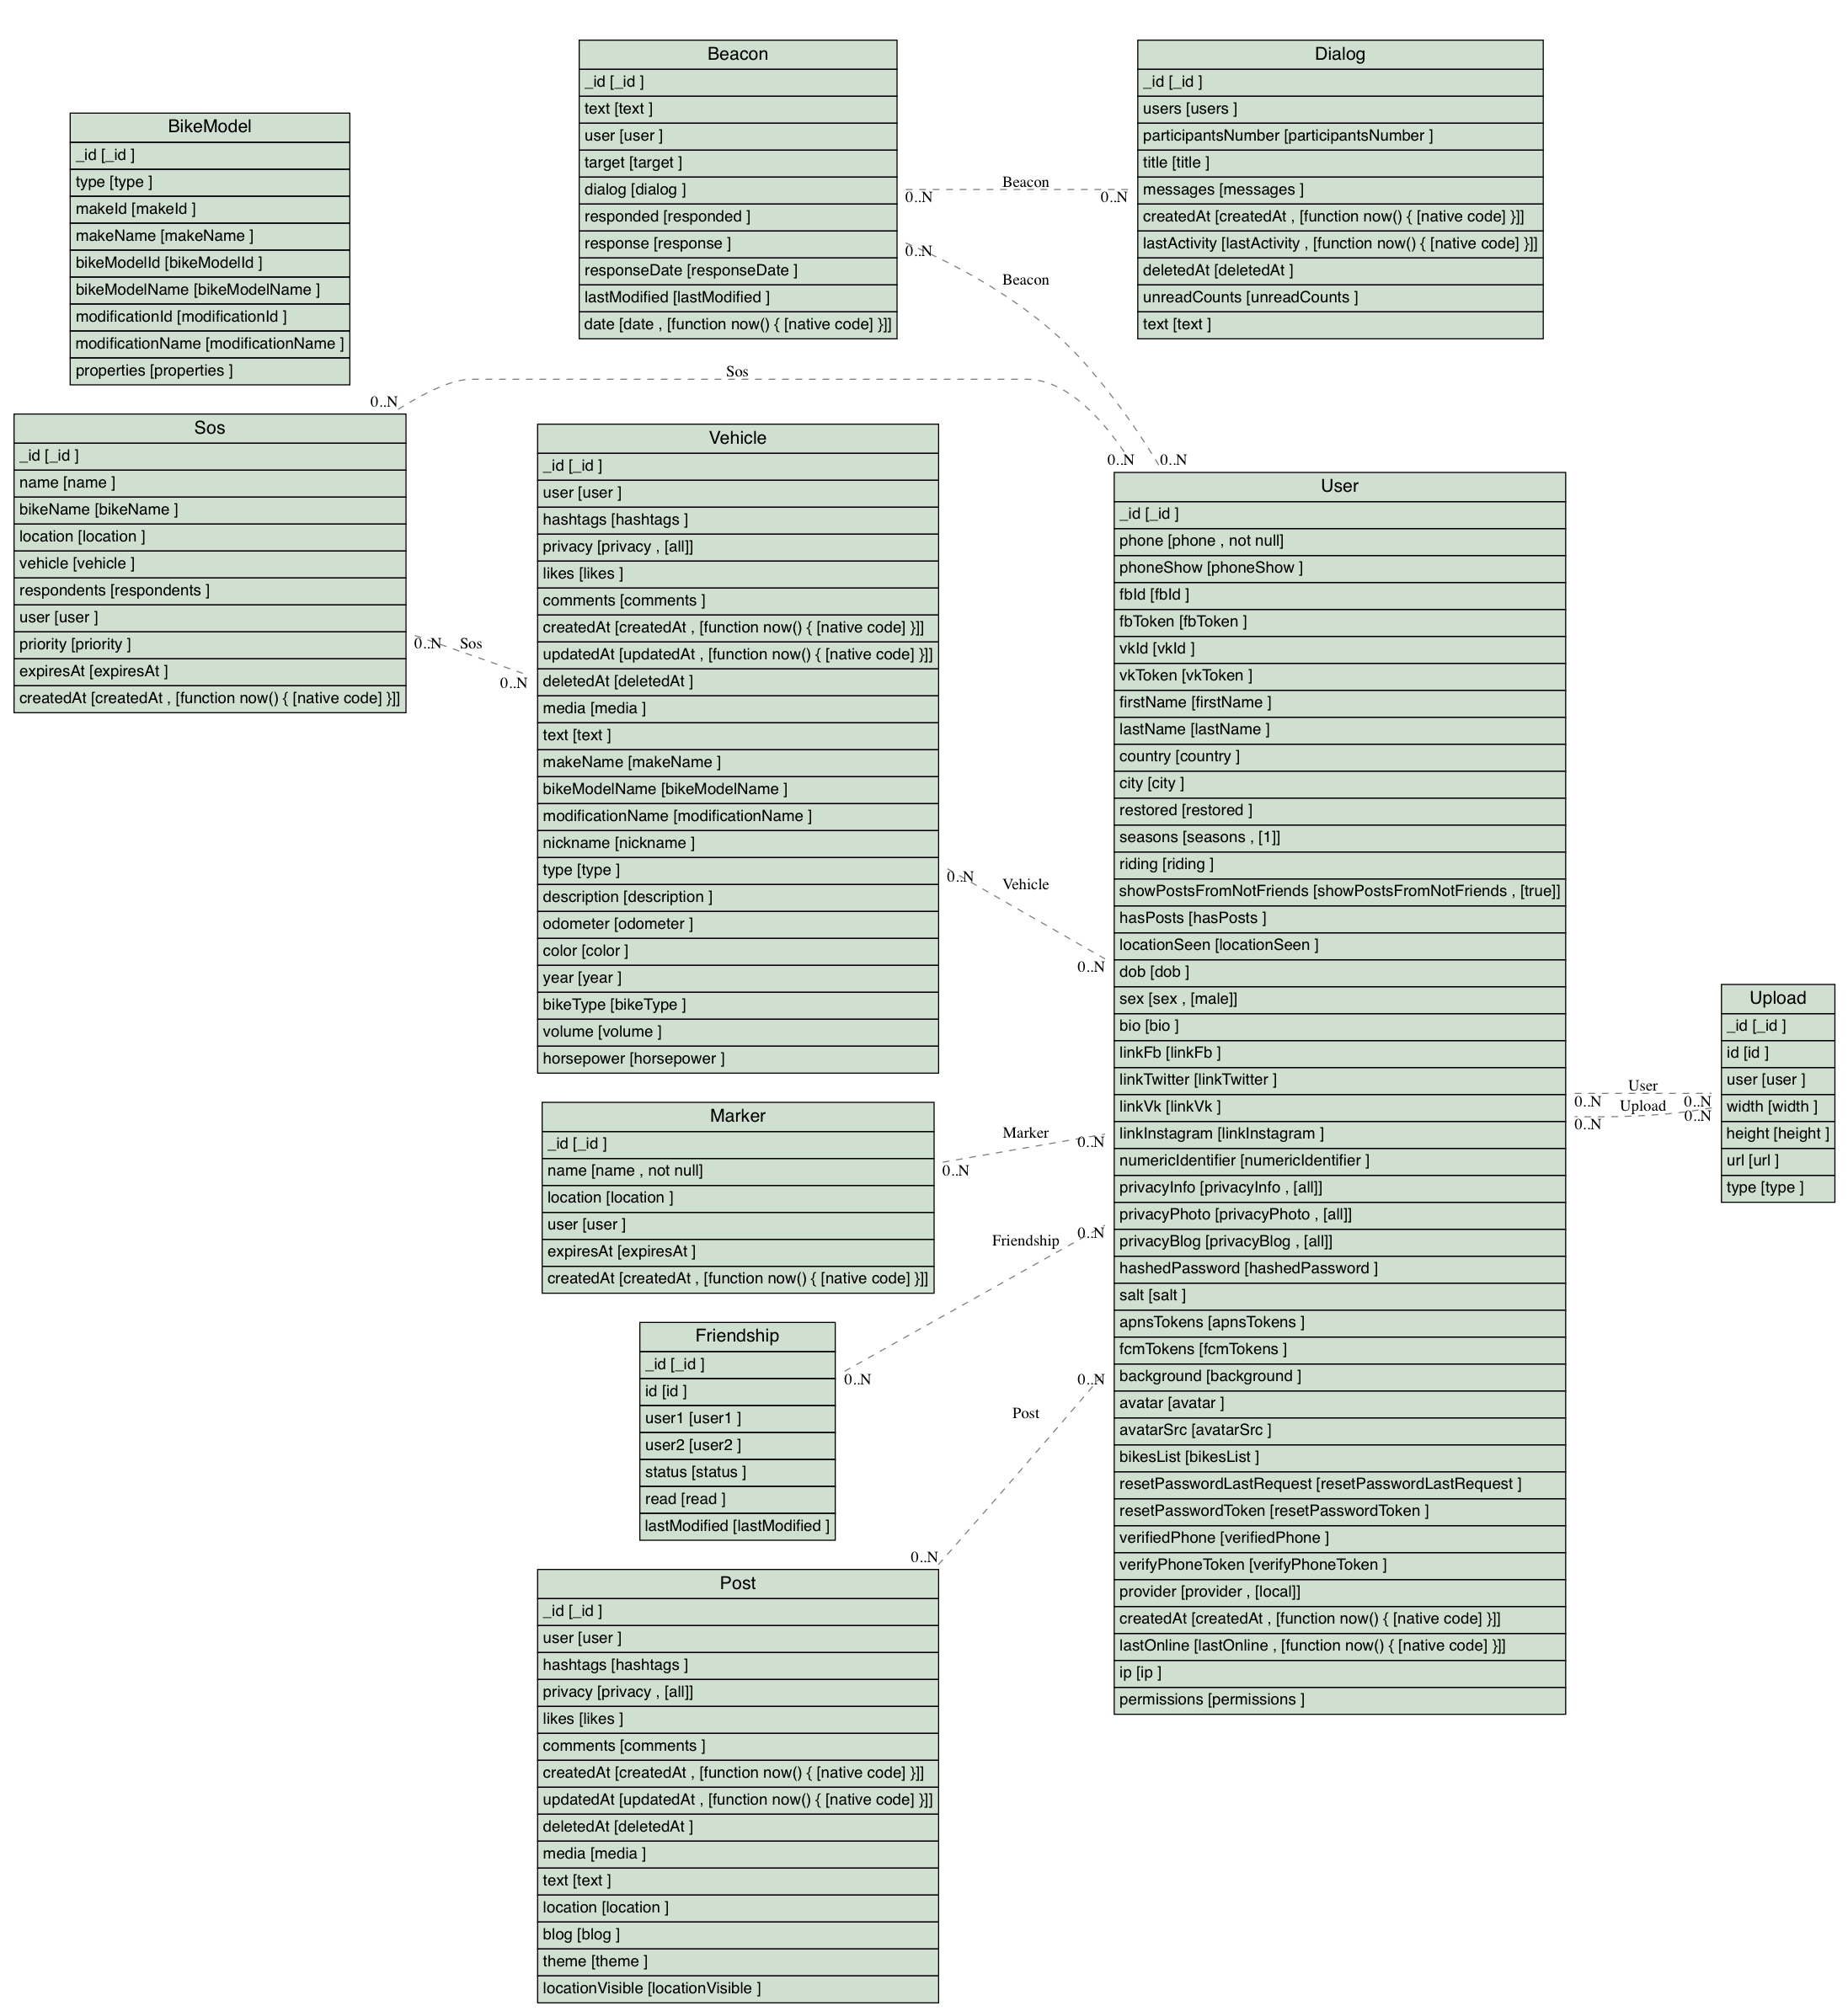
\includegraphics[scale=0.19]{erd.png}
	\caption{Инфологическая модель базы данных}
	\label{fig:domain:model:db:model}
\end{figure}

Важно отметить, что модель BikeModel используется для генирования набора существующих мотоциклов на стадии запуска серверного приложения. Это необходимо для удобного добавления мотоцикла из списка существующих, который представлен моделью Vehile. Информация о возможных мотоциклах сожержится на серверной части.

В информационной модели предусмотрены возможности для обеспечения безопасности аутентификации и авторизации: в модели User предусмотрены поля для хранения хешированного пароля и соли, а также токены от социальных сетей Facebook и <<ВКонтакте>>.

Метки сигалов SOS и предупреждения представлены моделью Marker. Важно отметить, что данная модель содержит даты создания маркера и его пропажи. Это сделано для того, чтобы не отображать огромное количество меток на карте. После прохождения определенного промежутка времени, заданного на сервере, они пропадают.

Сигнал SOS представлен отдельной моделью, содержит набор пользователей, которые откликнулись на сигнал помощи, приоритет: желтый или красный.

Функция переписки реализована с помощью модели Dialog, cодержит количество непрочитанных сообщений, количество участников диаога (на данный момент поддерживается только 2).

















	\section{Проектирование и разработка программного средства}
\label{sec:design}

\subsection{Разработка архитектуры}
\label{sec:design:architecture}

Классической архитектурой для мобильных приложений является двузвенная клиент-серверная архитектура. В простейшем случае единственная задача сервера -- возврат по запросу статической страницы с некоторой информацией. Однако в настоящее время данный подход устарел и используется в крайне простых приложениях: в основном для информационных сайтов~\cite{from_sites_to_webapps}. Абсолютное большинство ресурсов сети Интернет реализованы с высокой степенью интерактивности, то есть предоставляют некоторые элементы, с которыми пользователь может взаимодействовать. Таким образом, клиентская часть приложения, помимо простого отображения информации, должна быть управляемой с помощью пользовательских воздействий. Выбранная в пункте \ref{sec:analysis:specification:language} программная платформа позволяет нам это реализовать.

Вследствие интерактивности появляется необходимость в хранилище\linebreakданных, которая обычно решается с помощью реляционных баз данных. В пункте \ref{sec:analysis:specification:language} указано, что в приложении будет использоваться MongoDB, которая может запускаться на физически отдельной ЭВМ. Таким образом, приходим к трехзвенной архитектуре, схема которой представлена на рисунке~\ref{fig:analysis:specification:language:3-tier}.

\begin{figure}[ht]
\centering
	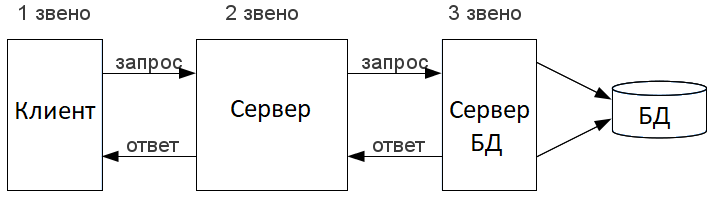
\includegraphics[scale=0.85]{3-tier.png}
	\caption{Вариант трехзвенной архитектуры}
	\label{fig:analysis:specification:language:3-tier}
\end{figure}

Появляется вопрос о необходимости серверной части приложения. Клиентская часть с помощью, например, протокола HTTP может сама без промежуточных звеньев обращаться к базе данных. Однако от данной модификации архитектуры было решено отказаться, поскольку появлются существенные риски нарушения требований безопасности: потребовалось бы наличие открытого API для взаимодействия клиента с БД, которое могло бы легко использоваться злоумышленником. В нашем случае серверная часть реализует так называе <<middleware>> (промежуточные звенья). При любом запросе со стороны клиентской части серверная, прежде чем выполнить дейтвие, индентифицирует пользователя, с устройства которого был отправлен запрос. Если токен пользователя совпадает с токеном, хранящимся на сервере, то происходит дальнейшее выполнение запроса. В противном случае возращается ответ с ошибкой.


% \subsection{Разработка даталогической и физической моделей базы данных}
\label{sec:design:db}

Как было упомянуто ранее, в программном средстве, описываемом данным дипломным проектом, будет использоваться специализированная СУБД \nezaboodka. Описание схемы БД для нее производится с помощью специальной нотации. Тем не менее, разрабатывать модель схемы можно с помощью любых средств, однако затем разработанную модель нужно вручную перевести в формат, используемый СУБД. 

На даталогическом уровне модель предметной области представляется в привязке к конкретной СУБД и описывает способ организации данных безотносительно их физического размещения. Описывать модель можно с помощью специальных графических нотаций~\cite{kulikov_db_workbook}. 

Модель даталогического уровня разработаем на основании инфологической модели, описание которой приведено в пункте \ref{sec:domain:model:db}. 

СУБД \nezaboodka разрабатывалась с расчетом на использование программистами в своих приложениях специальной клиентской библиотеки на языке \csharp. В связи с этим большинство стандартных типов данных одноименны представленным в данном ЯП. Кроме того, данная СУБД предлагает уникальный вариант ее использования. Первоначально, по разработанной в специальной нотации схеме БД генерируется исходный код классов модели. Данный исходный код можно включить свой проект и использовать данные классы модели как обычные регулярные классы. Затем, для сохранения экземпляров классов или их последующего поиска и извлечения и используется клиентская библиотека, которая сериализует экземпляры классов при передаче и десериализует их при получении. Таким образом, взаимодействие с данной СУБД несколько отличается от взаимодействия с традиционным SQL решениями. Но это даёт определенные преимущества. Например, появляется возможность использовать сколь угодно сложные структуры данных и легко сохранять и извлекать их. Таким образом, даталогическую модель используемой в разрабатываемом приложении БД можно проектировать с использованием традиционной диаграммы классов \uml.

Описание схемы БД в специальной нотации, используемой в \nezaboodka, приведено в приложении \dbschemeappendix. 

Можно выделить несколько особенностей данной схемы. 

Модель базы данных при разработке подверглась некоторой денормализации. Чаще всего она выражалась в добавлении дополнительных ссылок одних объектов на другие. Причинами такого решения являются следующие:

\begin{itemize}
	\item попытка повысить соответствие модели предметной области;
	\item упрощение манипуляций с данными.
\end{itemize}

Можно заметить, что достаточно часто в качестве типа поля используется тип Byte. Его использование означает, что данные поля смогут принимать только некоторые определенные значения. Вместо использования типов перечисления было принято решение использовать простой целочисленный тип, поскольку СУБД \nezaboodka предоставляет возможность создания специальных справочников. Данная СУБД изначально проектировалась как распределенная, а справочники -- это данные, которые будут храниться на всех узлах.

Необычным для регулярных SQL баз данных является использование списков в качестве типов полей. Как было сказано ранее, возможность из использования появилась вследствие поддержки СУБД сложных агрегирующих типов.

Вследствие этого можно заметить еще одно проявление денормализации: в некоторой дочерней сущности содержится ссылка на родительскую, а родительская содержит список дочерних. Опять же, данное решение вследствие отсутствии необходимости поиска позволит значительно повысить производительность при выборке данных.

Физический уровень моделирования БД описывает конкретные таблицы, связи, индексы, методы хранения, настройки производительности, безопасности. Описывать модель можно с помощью средств, уместных для предметной области~\cite{kulikov_db_workbook}. 

Индексы -- это специальные структуры, применяемые для ускорения операций взаимодействия с данными. В СУБД \nezaboodka они имеют название вторичных индексов. Целесообразно реализовать следующие индексы:

\begin{itemize}
	\item по названиям университетов, административных отделов, факультетов, кафедр, специальностей;
	\item по соответствующим аббревиатурам;
	\item по фамилии и имени пользователей;
	\item по дню недели и времени начала занятий;
	\item по номеру и году поступления групп.
\end{itemize}

Для идентификации используется специальное поле id, которое внедряется во все сущности с помощью наследования от сущности Entity.

Остальные настройки будут применяться непосредственно при развертывании программной системы, поэтому в данном разделе не\linebreakрассматриваются.


\subsection{Проектирование и разработка серверной части программного средства}
\label{sec:design:server}

\subsubsection{} Программный интерфейс серверной части
\label{sec:design:server:interface}

Предварительным условием для проектирования серверной части приложения является определение его интерфейса в высокоуровневых терминах предметной области. Таким образом, далее приведены методы его API, которые основаны на функциональных требованиях, определенных в подразделе~\ref{sec:domain:specification}:

\begin{itemize}
	\item метод регистрации пользователя системы, принимающий адрес электронной почты, хеш-сумму пароля, строку соли и название применявшегося алгоритма хеширования;
	\item метод смены пароля, также принимающий хеш-сумму пароля, соль и название алгоритма;
	\item метод смены пользователем электронной почты;
	\item метод аутентификации, принимающий хеш пароля и адрес электронной почты;
	\item метод восстановления пароля, принимающий адрес электронной почты;
	\item метод извлечения персональных данных пользователей;
	\item метод изменения фамилии, имени, отчества пользователя;
	\item метод изменения значения поля <<О себе>> пользователя;
	\item метод смены роли пользователя, принимающий объект сущности пользователя и роль, которую желается установить;
	\item метод подачи заявки на роль студента, принимающий номер группы;
	\item метод подачи заявки на роль преподавателя, в качестве параметра в котором выступает объект кафедры, сотрудником которой является преподаватель;
	\item методы подтверждения и отклонения заявок студентов;
	\item методы подтверждения и отклонения заявок преподавателей;
	\item метод, принимающий диапазон дат и номер группы и возвращающий список занятий;
	\item метод, который аналогичен предыдущему, но принимающий вдобавок номер подгруппы;
	\item метод, принимающий диапазон дат и фамилию, имя и отчество преподавателя и возвращающий список его занятий;
	\item метод, возвращающий список изучаемых студентов дисциплин;
	\item метод, возвращающий список дисциплин преподавателя;
	\item метод создания индивидуального задания преподавателем, принимающий номера групп и файл с условием задания;
	\item методы модификации условия индивидуального задания, включающие поиск и собственно изменение;
	\item метод отправки результатов выполнения заданий студентом;
	\item метод отклонения результатов задания преподавателем;
	\item метод оценивания результатов;
	\item метод извлечения всех результатов выполнения заданий, полученных и не проверенных преподавателем;
	\item метод добавления преподавателем файла учебно-методических материалов;
	\item метод получения прогресса выполнения заданий по всем предметам студента, в том числе полученные оценки (при их наличии);
	\item метод отправки сообщения одного пользователя другому;
	\item метод отправки сообщения с прикреплением;
	\item метод получения списка сообщения, переданных между двумя пользователями, принимающий помимо идентификационных номеров пользователей число сообщения для возврата и смещение, с какого сообщения начинать их выборку;
	\item метод создания объявления пользователя;
	\item метод извлечения объявлений пользователя, также принимающий их число и номер, с которого начинать выборку;
	\item метод получения списка студентов;
	\item метод получения списка студентов с их оценками по индивидуальным заданиям, а также с отметками посещения;
	\item метод совершения проверки посещения группой занятия;
	\item метод поиска пользователей;
	\item метод поиска преподавателей;
	\item метод поиска факультетов;
	\item метод поиска кафедр;
	\item метод поиска групп студентов;
	\item метод, возвращающий все группы факультета;
	\item методы выборки, создания и модификации специальностей\linebreakфакультета;
	\item методы выборки, создания и модификации программ специальностей.
\end{itemize}

На рисунке~\ref{fig:design:server:interface:server_algorithm} приведена схема алгоритма обработки запросов перечисленных методов программного интерфейса серверной частью приложения. Далее приведены архитектурные решения, которые были применены при реализации данной части программной системы. 

\begin{sidewaysfigure}
\centering
	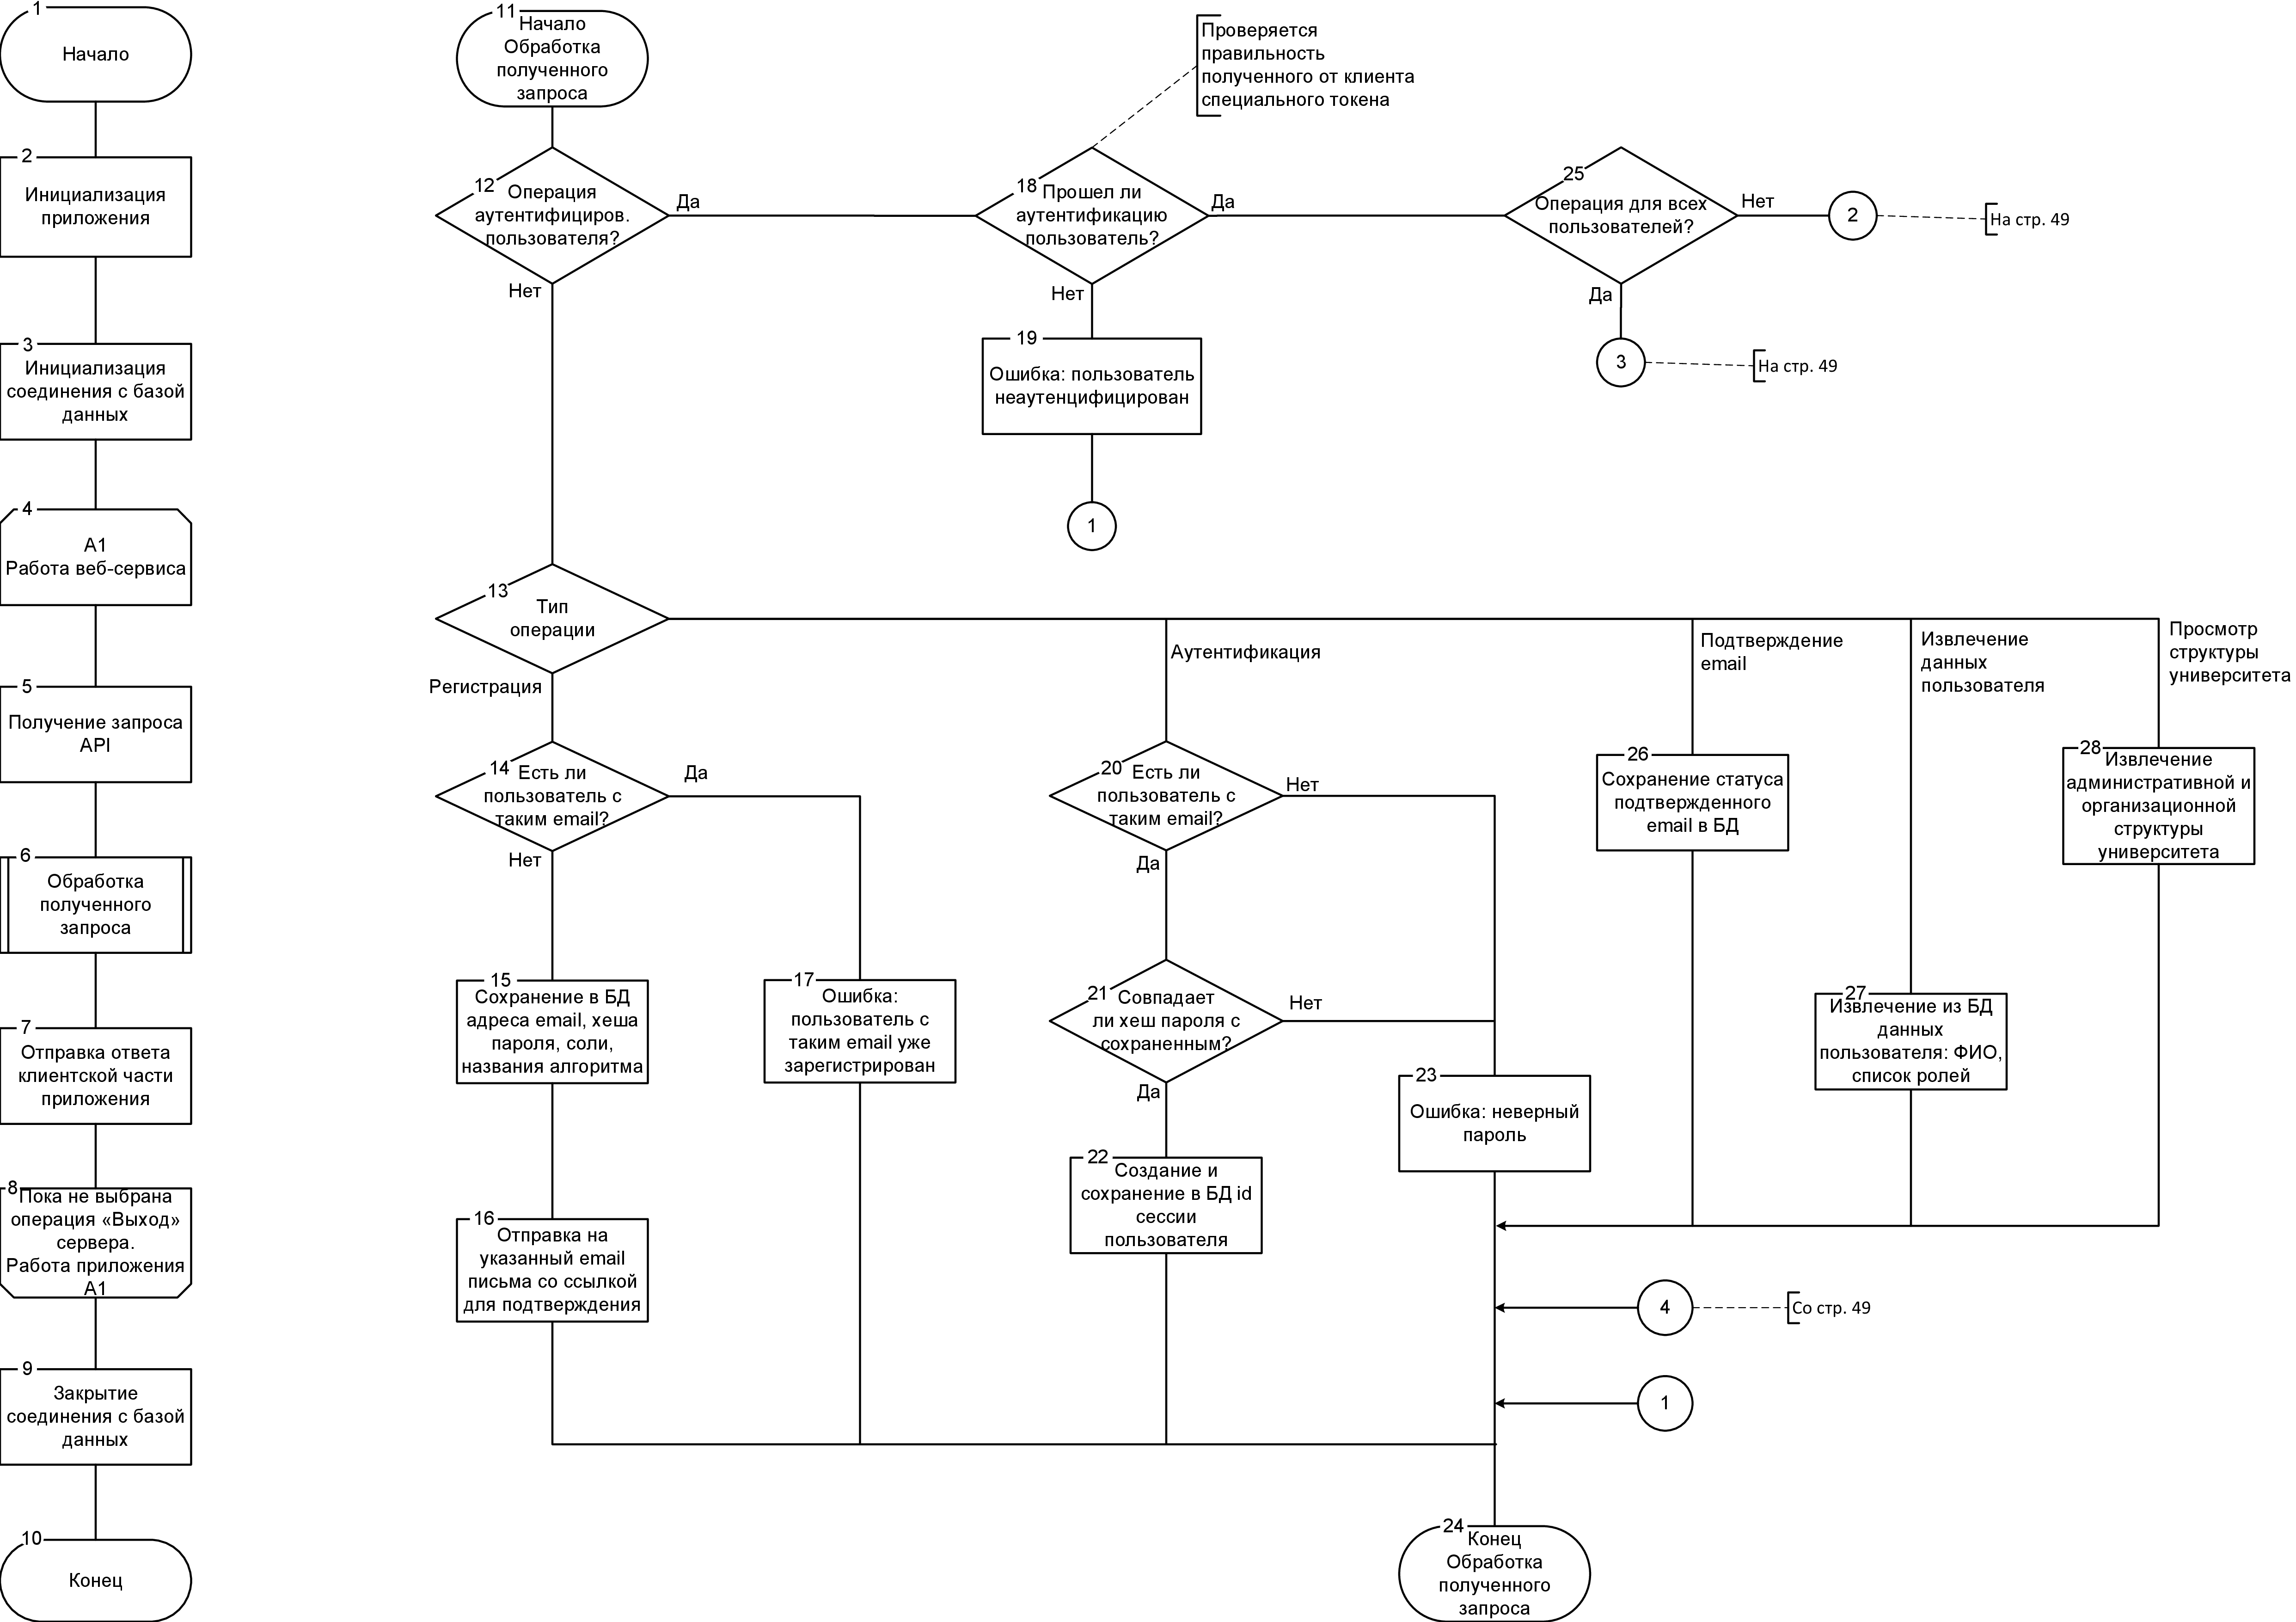
\includegraphics[scale=0.275]{server_algorithm_1.png}
	\caption{Схема программы серверной части программного средства}
	\label{fig:design:server:interface:server_algorithm}
\end{sidewaysfigure}

\begin{sidewaysfigure}
\ContinuedFloat
\centering
	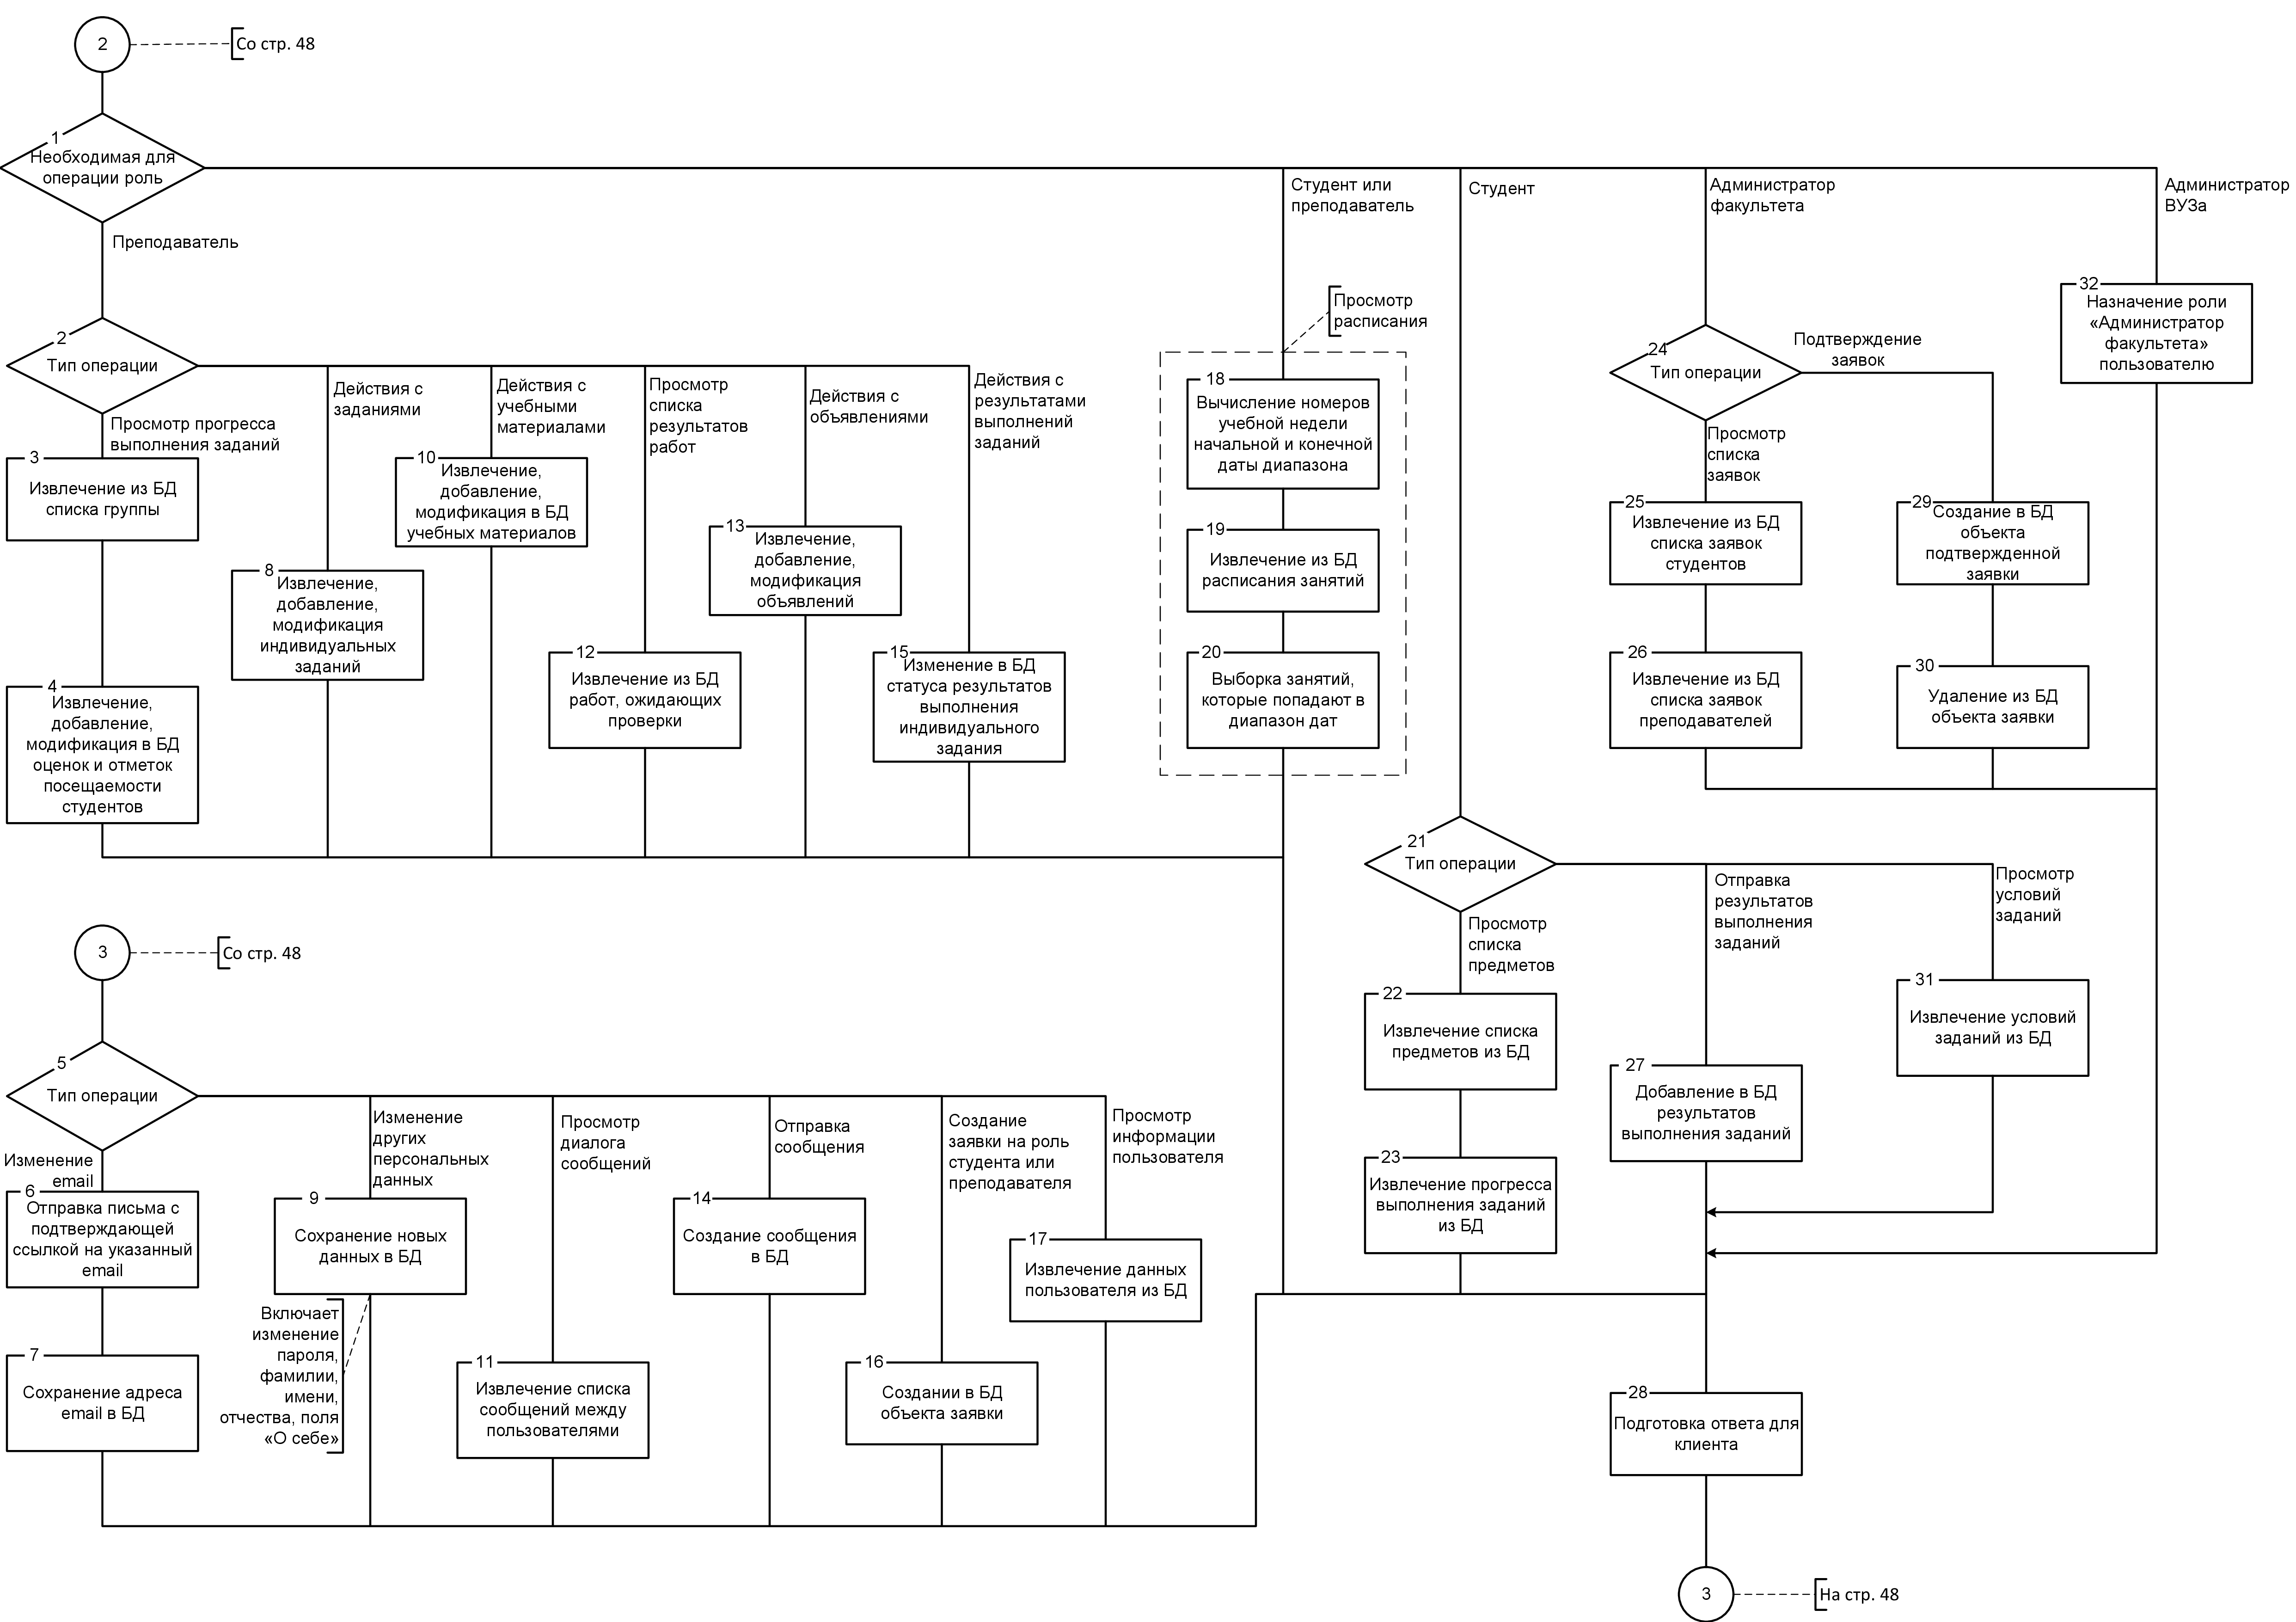
\includegraphics[scale=0.275]{server_algorithm_2.png}
	\caption{Схема программы серверной части программного средства (окончание)}
\end{sidewaysfigure}

Поскольку в ПС проектируется реализация сложных независимых систем ролей и пользовательских функций, которые находят своё отражение в серверной части приложения, то встаёт вопрос об их сопряжении. А поскольку данное сопряжение вследствие особенностей предметной области является достаточно нетривиальным: часть функций уникальна для некоторых функций, часть разделяется ими всеми. Поэтому целесообразным является разбиение их на следующие группы:

\begin{enumerate}
	\item функции, доступные без аутентификации;
	\item функции, доступные для всех аутентифицированных пользователей;
	\item функции студентов;
	\item функции преподавателей;
	\item функции студентов и преподавателей;
	\item функции администраторов факультетов;
	\item функции администраторов ВУЗов.
\end{enumerate}

Часть алгоритма, отвечающее за извлечение расписания занятий из БД, реализована на примере БГУИР, в котором занятия происходят по одной из 4 учебных недель, отсчет которых начинается с 1-го сентября.

Серверная проверка аутентификации пользователей будет осуществляться с помощью технологии создания и проверки специального токена.

Большое количество блоков, в которых осуществляется доступ к БД, подтверждает назначение всей серверной части приложения: прослойка между клиентским веб-приложением и базой данных с добавлением проверок аутентификации и авторизации.

Реализовав перечисленные методы API, можно будет достигнуть очень важной цели: внутренняя бизнес-логика, логика доступа к данным и сами данные будут надежно защищены.

\subsubsection{} Выбор протоколов коммуникации
\label{sec:design:server:protocols}

Можно выделить два основных стиля, которые (с необходимыми модификациями в каждом конкретном случае) применяются в информационных системах, содержащих веб-сервисы~\cite{applicationArchitectureGuide}: REST (Representational State Transfer -- протокол передачи состояния представления) и SOAP (Simple Object Access Protocol -- простой протокол доступа к объектам). Технически REST является архитектурным шаблоном проектирования, построенным на основе использования простых глаголов (называемых запросами или методами). На практике данный архитектурный стиль применяется в связке с протоколом прикладного уровня модели OSI HTTP. SOAP же является XML-ориентированным протоколом, причем стандарт не специфицирует применяемые протоколы передачи данных.

Основное отличие между данными протоколами состоит в способе манипулирования состоянием. SOAP предусматривает осуществление переходов между различными состояниями с помощью взаимодействия с единственной конечной точкой ввода информации, через которую предоставляется доступ к функциональности сервиса. Протокол REST предполагает использование ограниченного набора операций, которые могут применяться к ресурсам, адресуемым с помощью уникальных адресов URI. 

Данный протокол в большей степени соответствует распределенной архитектуре клиент-серверных приложений, поскольку серверная часть публично доступна для множества заведомо неизвестных клиентских приложений. REST обладает свойством отсутствия состояния, что означает, что каждый запрос должен содержать в себе достаточный набор данных для его осуществления. Кроме того, данный протокол не запрещает использование различных форматов передачи данных, например, JSON, что оказывается огромным преимуществом перед SOAP вследствие планируемого использования в клиентской части языка \typescript, который нативно поддерживает данный формат.


\subsection{Проектирование и разработка клиентской части программного средства}
\label{sec:design:client}

Задачи клиентской части приложения включают отображение пользовательского интерфейса и обработку действий пользователя. Типичными этапами его проектирования являются следующие~\cite[с.~78]{applicationArchitectureGuide}:

\begin{itemize}
	\item Идентификация типа клиентской части приложения, которое удовлетворяет установленным требованиям. Осуществление данного этапа осуществлено в подразделе~\ref{sec:design:architecture}.
	\item Выбор технологии пользовательского интерфейса. Осуществляется на основе анализа требуемой для реализации функциональности.
	\item Проектирование UI. Хорошей практикой является реализация модульности, а также принципа разделения ответственности компонентов.
	\item Определение стратегии и протоколов обмена информации между уровнями. Поскольку рассматриваемый уровень является самым верхним, а его протоколы связи с серверной частью приложения были рассмотрены в пункте~\ref{sec:design:server:protocols}, то данный вопрос считается решенным и рассматриваться не будет.
\end{itemize}

Ранее был проведен анализ и осуществлен выбор целевой платформы для реализации клиентской части приложения, был выбран основной язык программирования. Однако, существует огромное число специализированных технологий и фреймворков по созданию пользовательских интерфейсов. Представляется целесообразным провести уточнение средств разработки.

\subsubsection{} Уточнение выбора технологий программирования
\label{sec:design:client:technologies}

Язык программирования \typescript является надмножеством языка \js. Основной его особенностью является наличие проверок типов во время компиляции. Обычный \js код может быть скомпилирован \typescript компилятором (на выходе получится тот же самый код), однако по умолчанию данная возможность выключена, компилятор будет производить ошибку. Тем не менее, у разработчиков программного обеспечения есть возможность использования неимоверно большого числа \js библиотек и фреймворков, которая заключается в создании и использовании специальных файлов (их принято создавать с расширением .d.ts), которые содержат определения типов (type definitions) и создаются для каждой предназначенной к использованию библиотеки. Определенную проблему может представлять создание таких файлов: они бывают довольно громоздкими и их создание требует некоторых временных затрат. Тем не менее, существует проект по созданию таких файлов обычными разработчиками~\cite{githubDefinitelytyped}. В репозитории данного проекта находятся уже созданные .d.ts файлы для огромного числа существующих библиотек, что означает, что \typescript разработчики глубоко интегрированы в экосистему \js разработки.

Одной из широко используемых в настоящее время библиотек по созданию интерактивных интерфейсов веб-приложения является библиотека \react. Выбор в ее пользу был осуществлен вследствие наличия опыта по ее использованию у членов команды. Особенностями данной библиотеки являются следующие~\cite{habr_react_introduction}:

\begin{itemize}
	\item Кроссплатформенность. Переиспользование существующего кода\linebreakвозможно даже на других платформах благодаря проекту React Native.
	\item Декларативность: использование элементов (стандартных для \react \linebreak объектов, которые представляют собой HTML-теги) и компонентов (объекты, создаваемые разработчиком).
	\item JSX: техника создания и использования компонентов с помощью\linebreak HTML-подобного синтаксиса, который применяется прямо в \js коде.
	\item Виртуальный DOM: дерево \react элементов, которое отрисовывается в браузере, причем изменения в нём не требуют полной перерисовки всего интерфейса. Позволяет значительно улучшить быстродействие при использовании библиотеки.
\end{itemize}

Строго говоря, использование JSX является опциональным и может как не использоваться при разработке с \react, так и использоваться при разработке с помощью других библиотек. Однако, он значительно упрощает исходный код компонентов. Например, следующий \js код 
\begin{flushleft}
\qquad\qquad\qquad return <div>Hello\{this.props.children\}</div>;
\end{flushleft}
после компиляции будет преобразован в следующий
\begin{flushleft}
\qquad\qquad\qquad return React.createElement(\\
\qquad\qquad\qquad\qquad ``div'',\\
\qquad\qquad\qquad\qquad null,\\
\qquad\qquad\qquad\qquad ``Hello '',\\
\qquad\qquad\qquad\qquad this.props.children\\
\qquad\qquad\qquad );
\end{flushleft}

Лаконичность использования JSX очевидна. Некоторым кажется сомнительным данный подход, в котором смешивается исполняемый код и код разметки. Однако, данное смешение формирует исходный код представления. Кроме того, в других фреймворках используются специальные конструкции по реализации, например, циклов, условий, в то время как при использовании JSX нужды в новых конструкциях нет, ведь используются стандартные операторы языка \js (в текущем проекте -- \typescript).

Одна из классификаций компонентов \react предполагает их разделение на pure (простые) и stateful (имеющие внутреннее состояние)~\cite{react}. Простые компоненты, реализованные в виде классов, унаследованных от Re\-act.Com\-po\-nent, переопределяют метод render(), который принимает некоторый набор исходных данных и возвращает элемент, предназначенный для отображения. Компоненты другого класса имеют внутри себя некоторые данные, образующие их состояние. Чтобы \react узнал, что данные изменились, и осуществил перерисовку измененных компонентов, требуется использовать специальный метод this.setState(...). 

Для упрощения управления состоянием компонентов могут применяться различные техники. Одной из них является использование специальной библиотеки \mobx. Его идея заключается в недопущении неконсистентного состояния приложения, что достигается отслеживанием данной библиотекой всего дерева используемых объектов и обновлении интерфейса при любом их изменении. Рекомендуемый и наиболее удобный способ использования \mobx заключается в использовании специальных декораторов, с помощью которых помечаются классы, методы и поля классов. Не смотря на их официальный экспериментальный статус, они поддерживаются компилятором \typescript. В терминологии \mobx существуют следующие объекты программы:

\begin{itemize}
	\item \react компонент, который автоматически перерисовывается при изменении состояния. Помечается декоратором @observer.
	\item Объекты в классах, находящиеся под наблюдением библиотеки. Обозначаются с помощью декоратора @observable.
	\item Вычисляемые методы, возвращающие некоторое значение на основании состояния объекта или других вычисляемых методов. Подвергаются оптимизации со стороны \mobx. Обозначаются декоратором @computed.
	\item Методы, изменяющие состояние объектов. Обычно это некоторые операции ввода-вывода, а также передачи данных. Помечаются с помощью @ac\-ti\-on.
	\item Методы, которые должны автоматически запускаться при любых изменениях содержащихся в них данных. Типичный пример их использования: логгирующие операции. Обозначаются с помощью @autorun.
\end{itemize}

Однако, \mobx представляет собой только библиотеку. Ограничения на архитектуру приложения не накладываются, однако сохраняется\linebreak необходимость ее реализации программистом. Одним из вариантов является разбиение всех компонентов на контейнерные и презентационные~\cite{presentational_and_container_components}. Особенности создания презентационных компонентов следующие:

\begin{itemize}
	\item Их задача заключается в определении, как должны \emph{выглядеть} элементы.
	\item Не зависят от других частей приложения.
	\item Получают данные исключительно в качестве входных параметров.
	\item Не изменяют данные.
	\item Редко имеют собственное состояние (в таком случае это состояние UI, а не собственно данные).
	\item Обычно содержат JSX разметку и имеют относящиеся к ним стили.
\end{itemize}

В это же время особенности контейнерных компонентов заключаются в следующем:

\begin{itemize}
	\item Их задача заключается в определении, как элемент должны \emph{работать}.
	\item Предоставляют данные и методы их обработки другим компонентам.
	\item Как правило имеют некоторые данные в виде состояния.
	\item Обычно не содержат JSX разметки и никогда не имеют стилей.
\end{itemize}

Использование данного подхода имеет следующие преимущества:

\begin{itemize}
	\item Достигается выполнение принципа разделения ответственности.
	\item Появляется возможность легкого переиспользования компонентов с различными источниками данных.
	\item Одни и те же презентационные компоненты могут использоваться повсеместно в приложении.
	\item Презентационные компоненты формируют <<палитру>>. Их внешний\linebreak вид может изменяться без влияния на логику приложения.
\end{itemize}

Еще один важный момент относительно проектирования UI, помимо содержания и интерактивных пользовательских взаимодействий, касается стилизации внешнего вида компонентов. Существует несколько подходов по ее исполнению~\cite{styling_react}: использование внутренних (inline) и внешних стилей.

Первый подход имеет множество недостатков:

\begin{itemize}
	\item невозможно использование медиа-запросы, чтобы, например, реагировать на изменения ширины экрана или отличать мобильное устройство от настольного компьютера;
	\item невозможно использование псевдоклассов и псевдоэлементов, например: :hover, :active, :before, :after;
	\item значительное увеличение размера разметки и снижение производительности;
	\item невозможно переопределение стилей по более сложным селекторам.
\end{itemize}

Тем не менее, Facebook, как компания разработчик \react, несмотря на описанные недостатки, выступает за использование inline стилей. Причиной этому является стремление обеспечить единообразие с React Native, поскольку там возможность стилизации обеспечивается только данным подходом.

Второй подход -- использование внешних стилей -- является более традиционным для веб-разработки. Его эволюционное развитие включает несколько этапов:

\begin{itemize}
	\item Создание одного файла .css со стилями, который подключается один раз глобально в главный html файл. В React компонентах используется тег className со значениями имен классов из этого файла.
	\item Разбиение единого файла стилей на множество файлов в соответствии с реализованными компонентами. В файлы компонентов подключаются лишь те стили, которые там необходимы. Преимущества данного подхода заключаются в простоте поиска файла, в который необходимо внести изменения, и в простоте удаления компонентов и соответствующих им файлов стилей.
	\item Использование различных препроцессоров стилей, таких как\linebreak SASS/SCSS, LESS и прочих. 
\end{itemize}

Использование SASS по сравнению с обычным CSS предоставляет следующие преимущества~\cite{sass_guide}:

\begin{itemize}
	\item переменные, в которых можно хранить значения цветов, шрифтов, а также любые другие значения;
	\item вложенность, что приводит к большей наглядности файлов стилевых таблиц за счет соответствия иерархии HTML кода;
	\item фрагментирование, то есть обеспечение модульности;
	\item импортирование других файлов стилей, которое, в отличие от CSS, вместо создания новых HTTP запросов подставляет указанный файл в тот, где он вызывается, таким образом на выходе получается единственный файл стилей;
	\item примеси (mixins), которые представляют собой группы деклараций, используемые по нескольку раз;
	\item наследование, позволяющее привносить наборы свойств от одного селектора к другому;
	\item использование математических операторов.
\end{itemize}

Таким образом, на основании проведенного уточнения технологий для использования выбираем следующие: \react в связке с \mobx и SCSS, кроме того, для разметки в коде повсеместно будет использоваться JSX.

\subsubsection{} Проектирование клиентской части приложения
\label{sec:design:client:ux}

Далее рассмотрим вопрос взаимодействия пользователя с клиентской частью приложения. Известно, что удобство пользования программным средством может во многом определять успешность проекта в целом~\cite[с.~44]{code_complete}.

Схема работы клиентской части программной системы представлена на рисунке~\ref{fig:design:client:ux:client_algorithm}. Среди ее особенностей можно выделить в высокой степени соответствие диаграмме прецедентов, которая была составлена и рассмотрена в пункте~\ref{sec:domain:model:use_cases}. Кроме того, данный чертеж представляет собой отображение чертежа схемы серверной части с отличием в том, что там делается акцент на взаимодействие с базой данных, а в данном чертеже -- на отображении данных и интерактивном взаимодействии с пользователем. 

\begin{sidewaysfigure}
\centering
	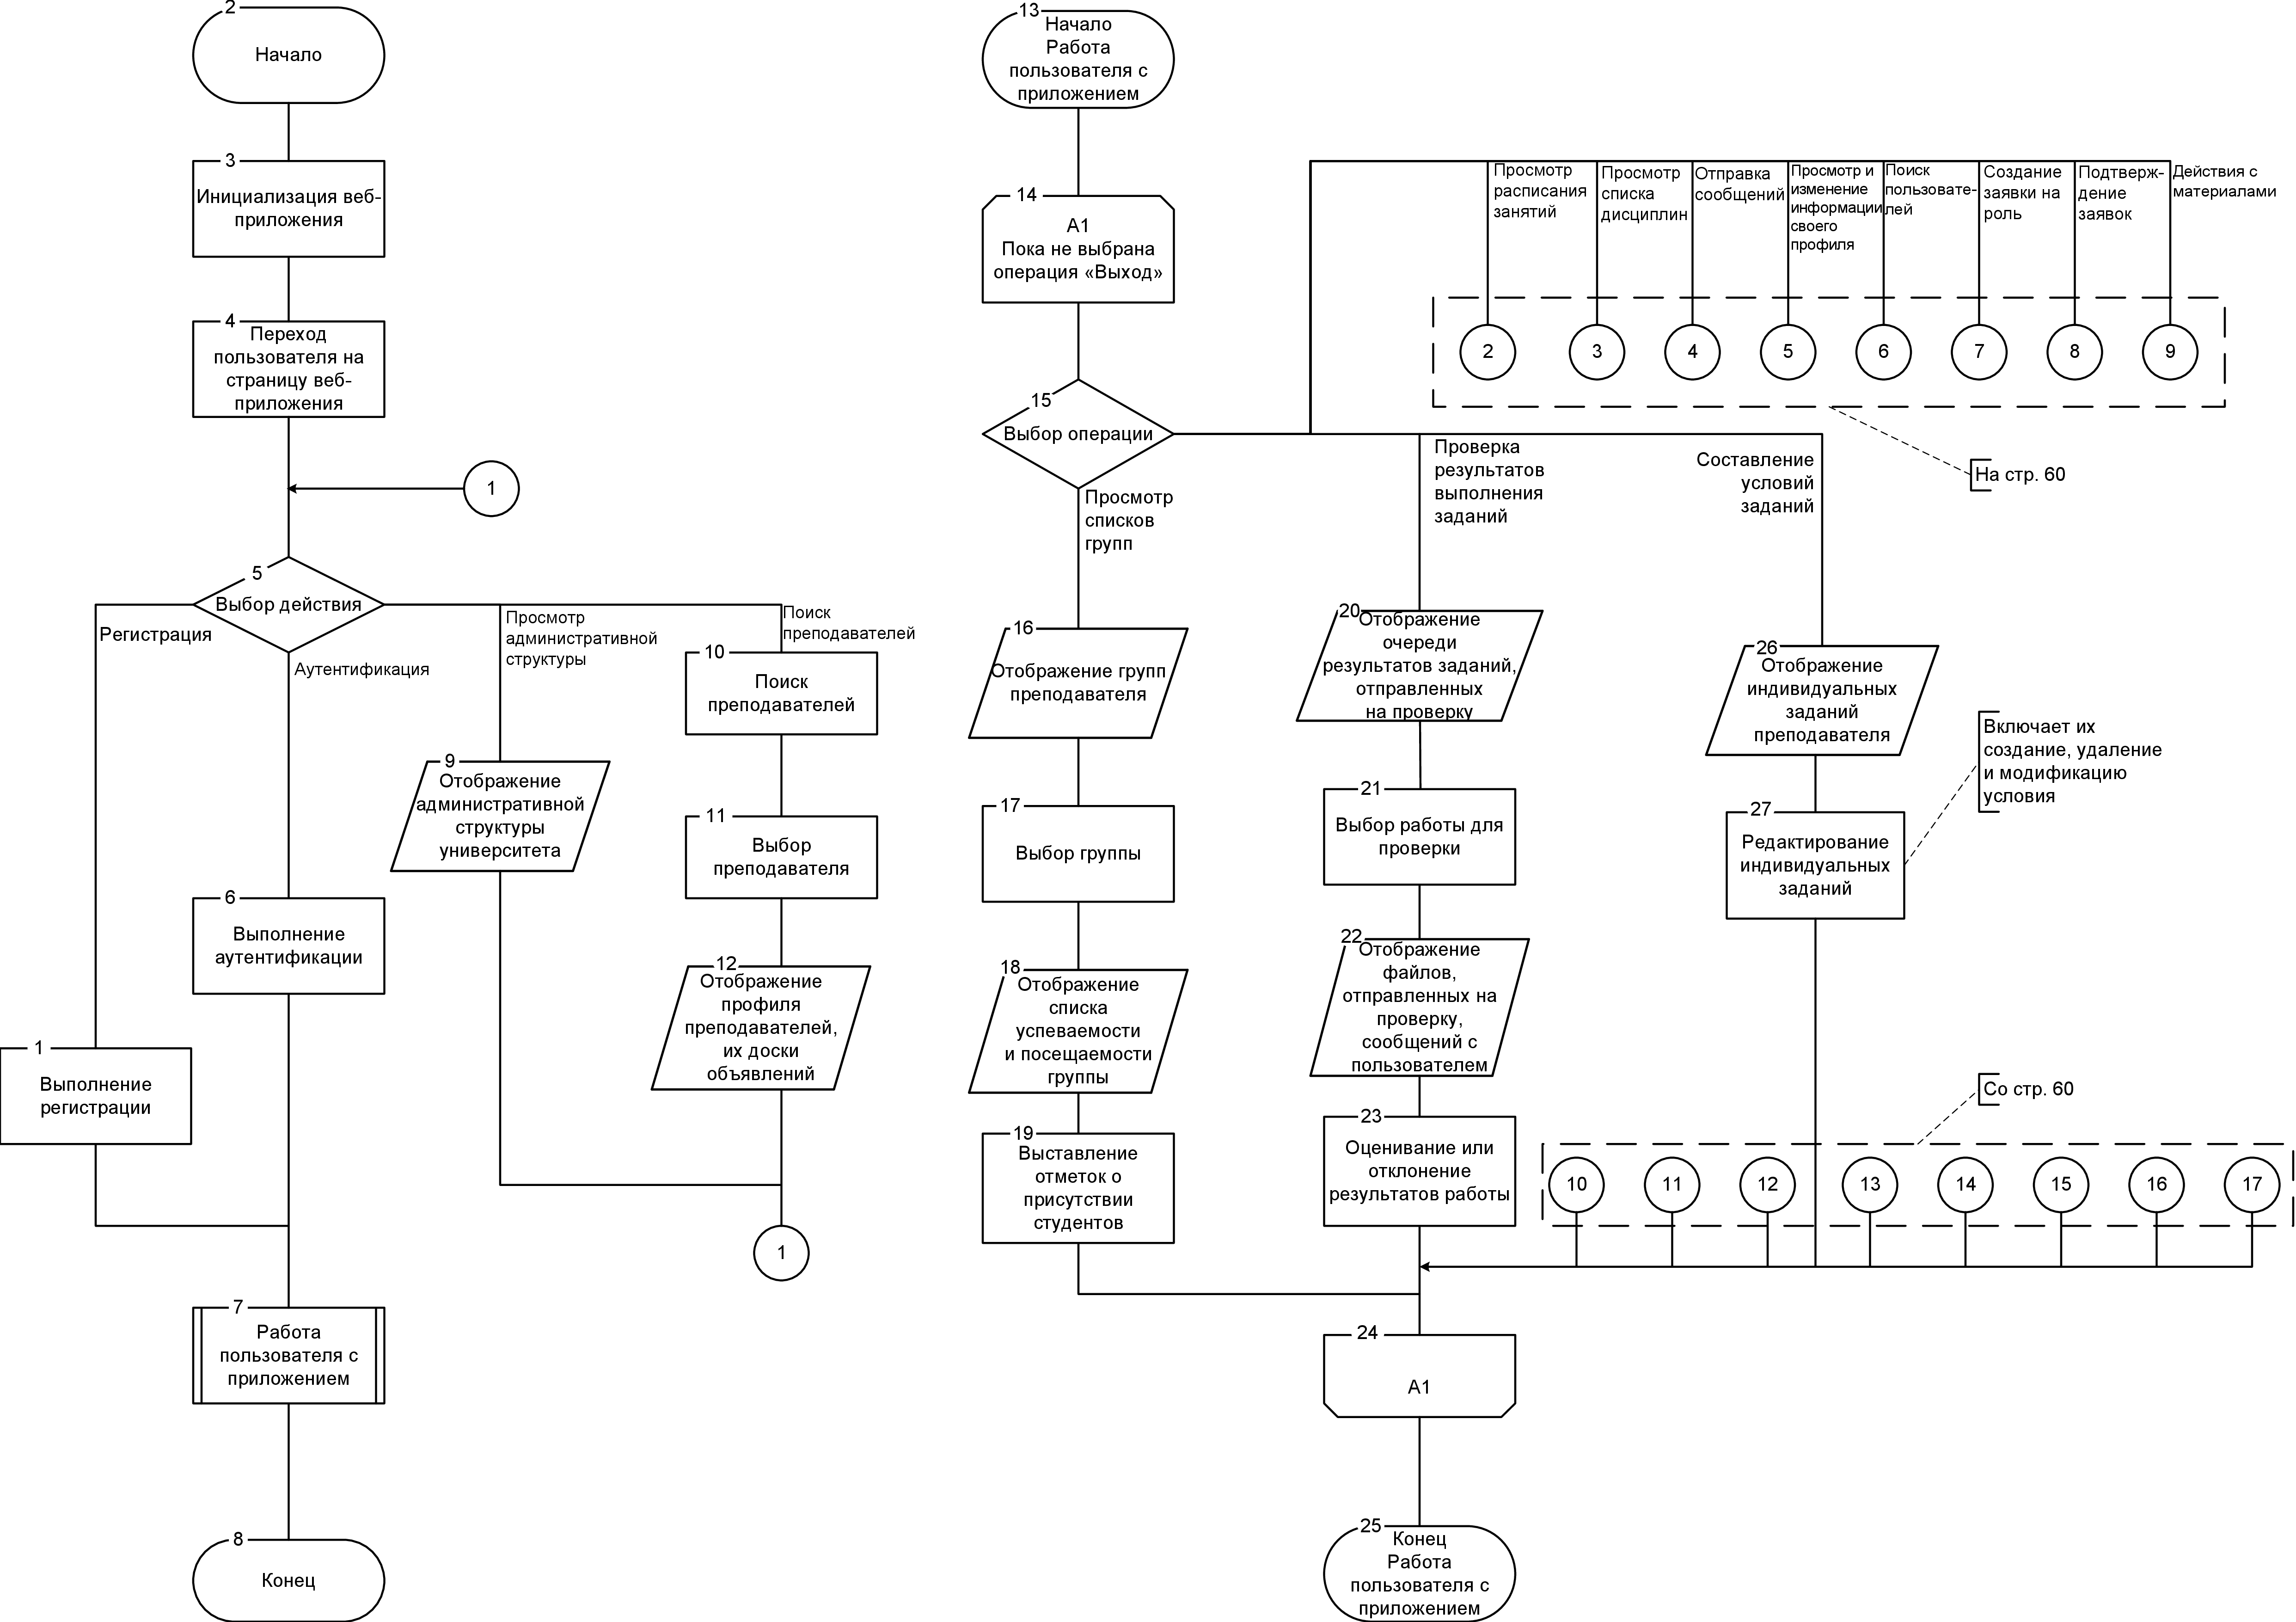
\includegraphics[scale=0.275]{client_algorithm_1.png}
	\caption{Схема программы клиентской части программного средства}
	\label{fig:design:client:ux:client_algorithm}
\end{sidewaysfigure}

\begin{sidewaysfigure}
\ContinuedFloat
\centering
	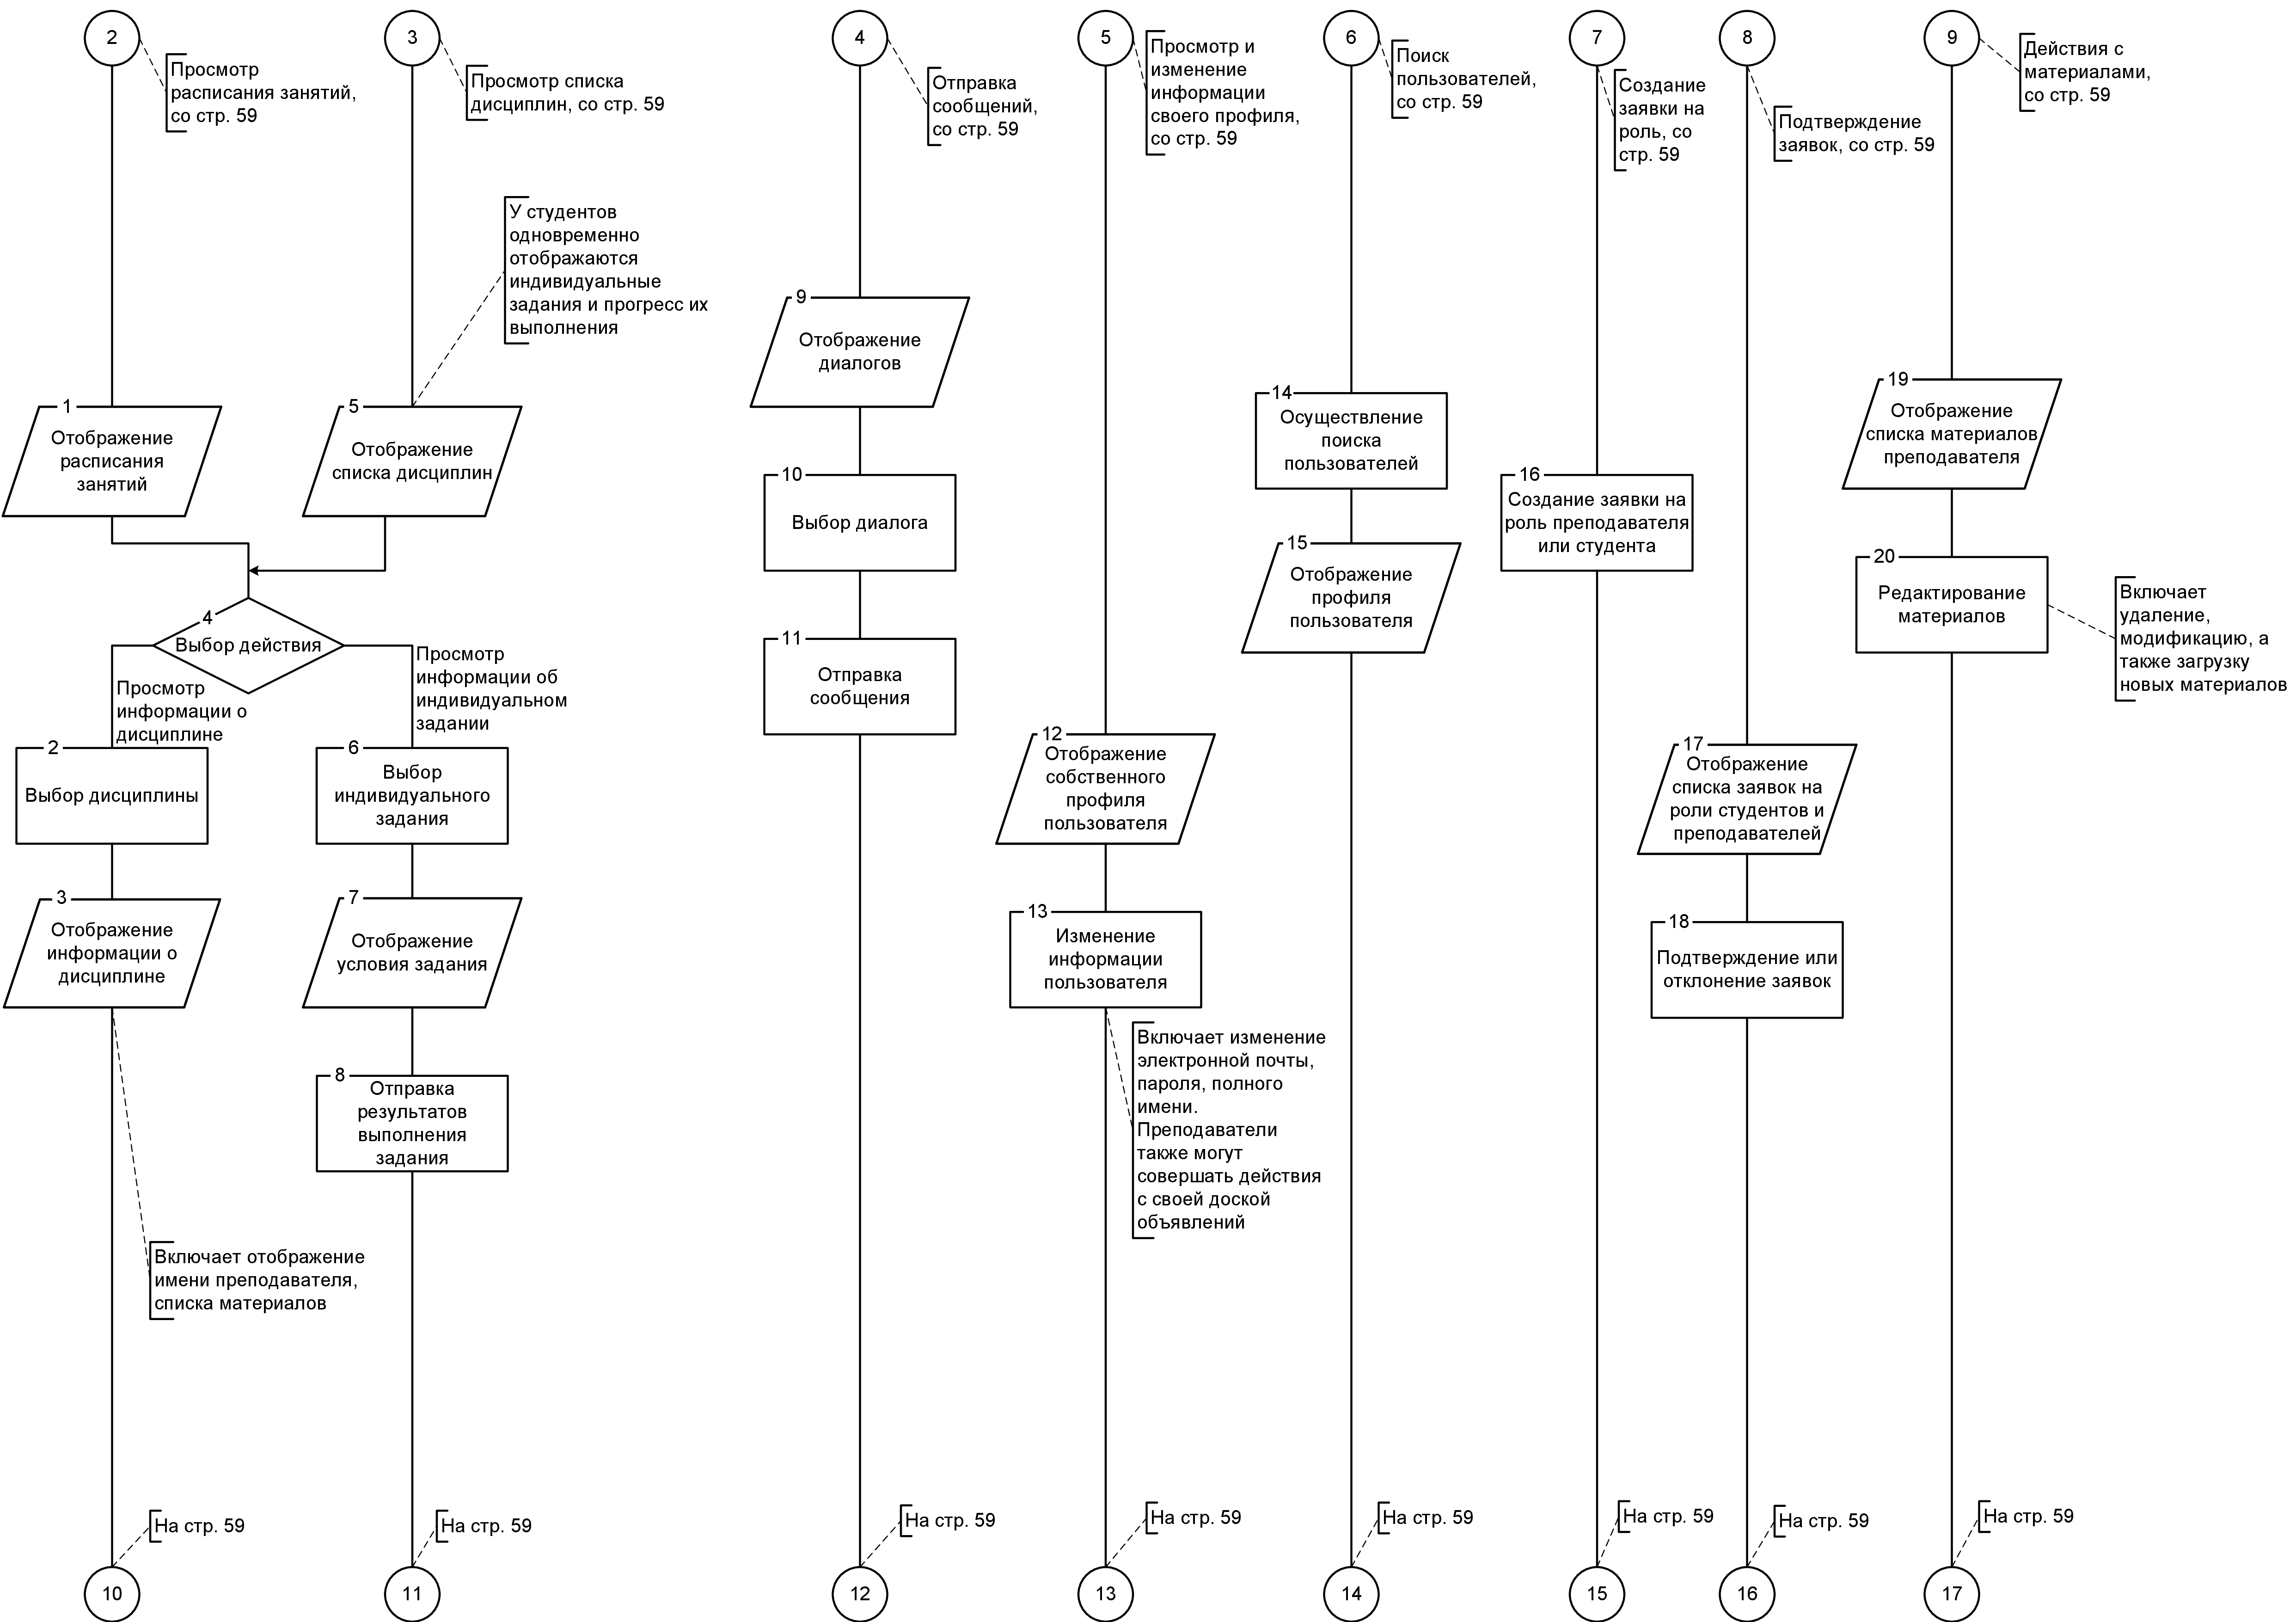
\includegraphics[scale=0.275]{client_algorithm_2.png}
	\caption{Схема программы клиентской части программного средства (окончание)}
\end{sidewaysfigure}

Таким образом, составленная схема клиентской части ПС будет использована при разработке навигации (routing) по страницам веб-приложе\-ния.

\subsubsection{} Конструирование клиентской части приложения
\label{sec:design:client:development}

Наконец, по завершению этапов проектирования и подготовки можно приступить к собственно созданию исходных кодов приложения. Ключевые фрагменты кода, описание которых приведено в данном пункте, приведены в приложении \sourcecodeappendix.

Для начала необходимо создать корневой файл index.html. Ключевая его особенность состоит в следующем теге
\begin{flushleft}
\qquad\qquad\qquad\qquad\qquad <div id=``root''></div>
\end{flushleft}

Несмотря на то, что он объявляется пустым, именно в него библиотека \react подставит всё приложение.

Кроме этого, в данном файле подключается основная зависимость приложения -- непосредственно сама библиотека \react и библиотека по управлению виртуальным деревом элементов браузера, а также пакет bun\-dle.js, в который будет собран весь созданный исходный код. Помимо библиотек, подключаются некоторые файлы стилей, необходимые для корректной работы некоторых компонентов, например, специальных шрифтов, предоставляющих возможность использования большого количества специальных иконок.

Следующий важный файл -- корневой файл исходного \typescript кода index.tsx. Единственная его цель -- вызов специального метода React\-DOM.ren\-der(), который и подставляет в указываемый тег каркас приложения.

Каркас приложения, определенный в файле App.tsx, представляет собой класс AppRouter, в котором и задаются пути маршрутизации страниц веб-приложения. В нем используется стандартный элемент Router, который при переходе пользователем по адресам приложения создаёт экземпляр класса App и передает в качестве его содержимого соответствующую страницу.

Задача компонента App -- рендеринг шапки сайта и бокового меню. В качестве дочерних для него \react подставляет такие компоненты, как Agenda (отображающий список расписания занятий), Disciplines (отображающий список дисциплин) и другие.

В качестве решения по организации пользовательского интерфейса был принят шаблон, состоящий из двух колонок. Таким образом, в левой колонке будут отображаться списки, а в правой -- детали выбранного из списка элемента. Кроме того, для повышения удобства пользования было выдвинуто требование, чтобы правая колонка не изменяла содержимого при переходах пользователем по страницам приложения. Данное требование удовлетворяется в связи с использованием библиотеки \react, поскольку она достаточно эффективно реализует механизм перерисовки только измененных областей. 

Задача дочерних компонентов класса App состоит в обращении к классам, обеспечивающим сетевое взаимодействие с сервером, получении от них данных, а затем создании <<чистых>> (pure) компонентов, которые эти данные отображают. При этом разработка производится путем движения сверху-вниз (от общих компонентов к очень маленьким частным), причем достигается высокая степень модульности: число уровней иерархии достигает не менее трех, и только самые частные компоненты отвечают за непосредственный вывод информации.

За хранение данных, а также их извлечение отвечают специальные классы, называемые <<хранилищами>> (stores). Данный подход предлагается в качестве лучших практик разработчиками библиотеки \mobx~\cite{mobx_best_practices}. Предлагаемый ими подход заключается в создании специальных классов, называемых хранилищами предметной области (domain stores), ответственных за определенные аспекты работы приложения, и разделении данных между ними. В данном дипломном проекте, такими аспектами являются хранение расписания, списка предметов, сообщений и так далее. Кроме того, предлагается создание еще одного хранилища, ответственного за хранение состояния интерфейса (UiStore), которое может хранить следующую информацию: сессионные данные, текущую тему приложения, язык (locale), разрешение экрана, состояние элементов интерфейса и так далее. Например, мы будем хранить в данном классе компоненты, ответственные за левую и правую колонку приложения.

Помимо кода компонентов, необходимо создать код их стилизации. Благодаря использованию SASS/SCSS можно достигнуть такой же степени модульности, что и при реализации компонентов. Поэтому часто классы компонентов имеют единственный им соответствующий файл стилей и импортируют лишь его.

Таким образом, разработает исходные коды клиентской части приложения. 


\subsection{Развертывание программного средства}
\label{sec:design:deployment}

После выявления, а также завершения проектирования всех компонентов программного средства появляется вопрос о планировании развертывания всей системы. Необходимо составить описание требуемых аппаратно-программных комплексов, которые понадобятся для обеспечения функционирования распределенного приложения. Для этих целей целесообразным выглядит составление диаграммы развертывания стандарта \uml. 

\begin{figure}[H]
\centering
	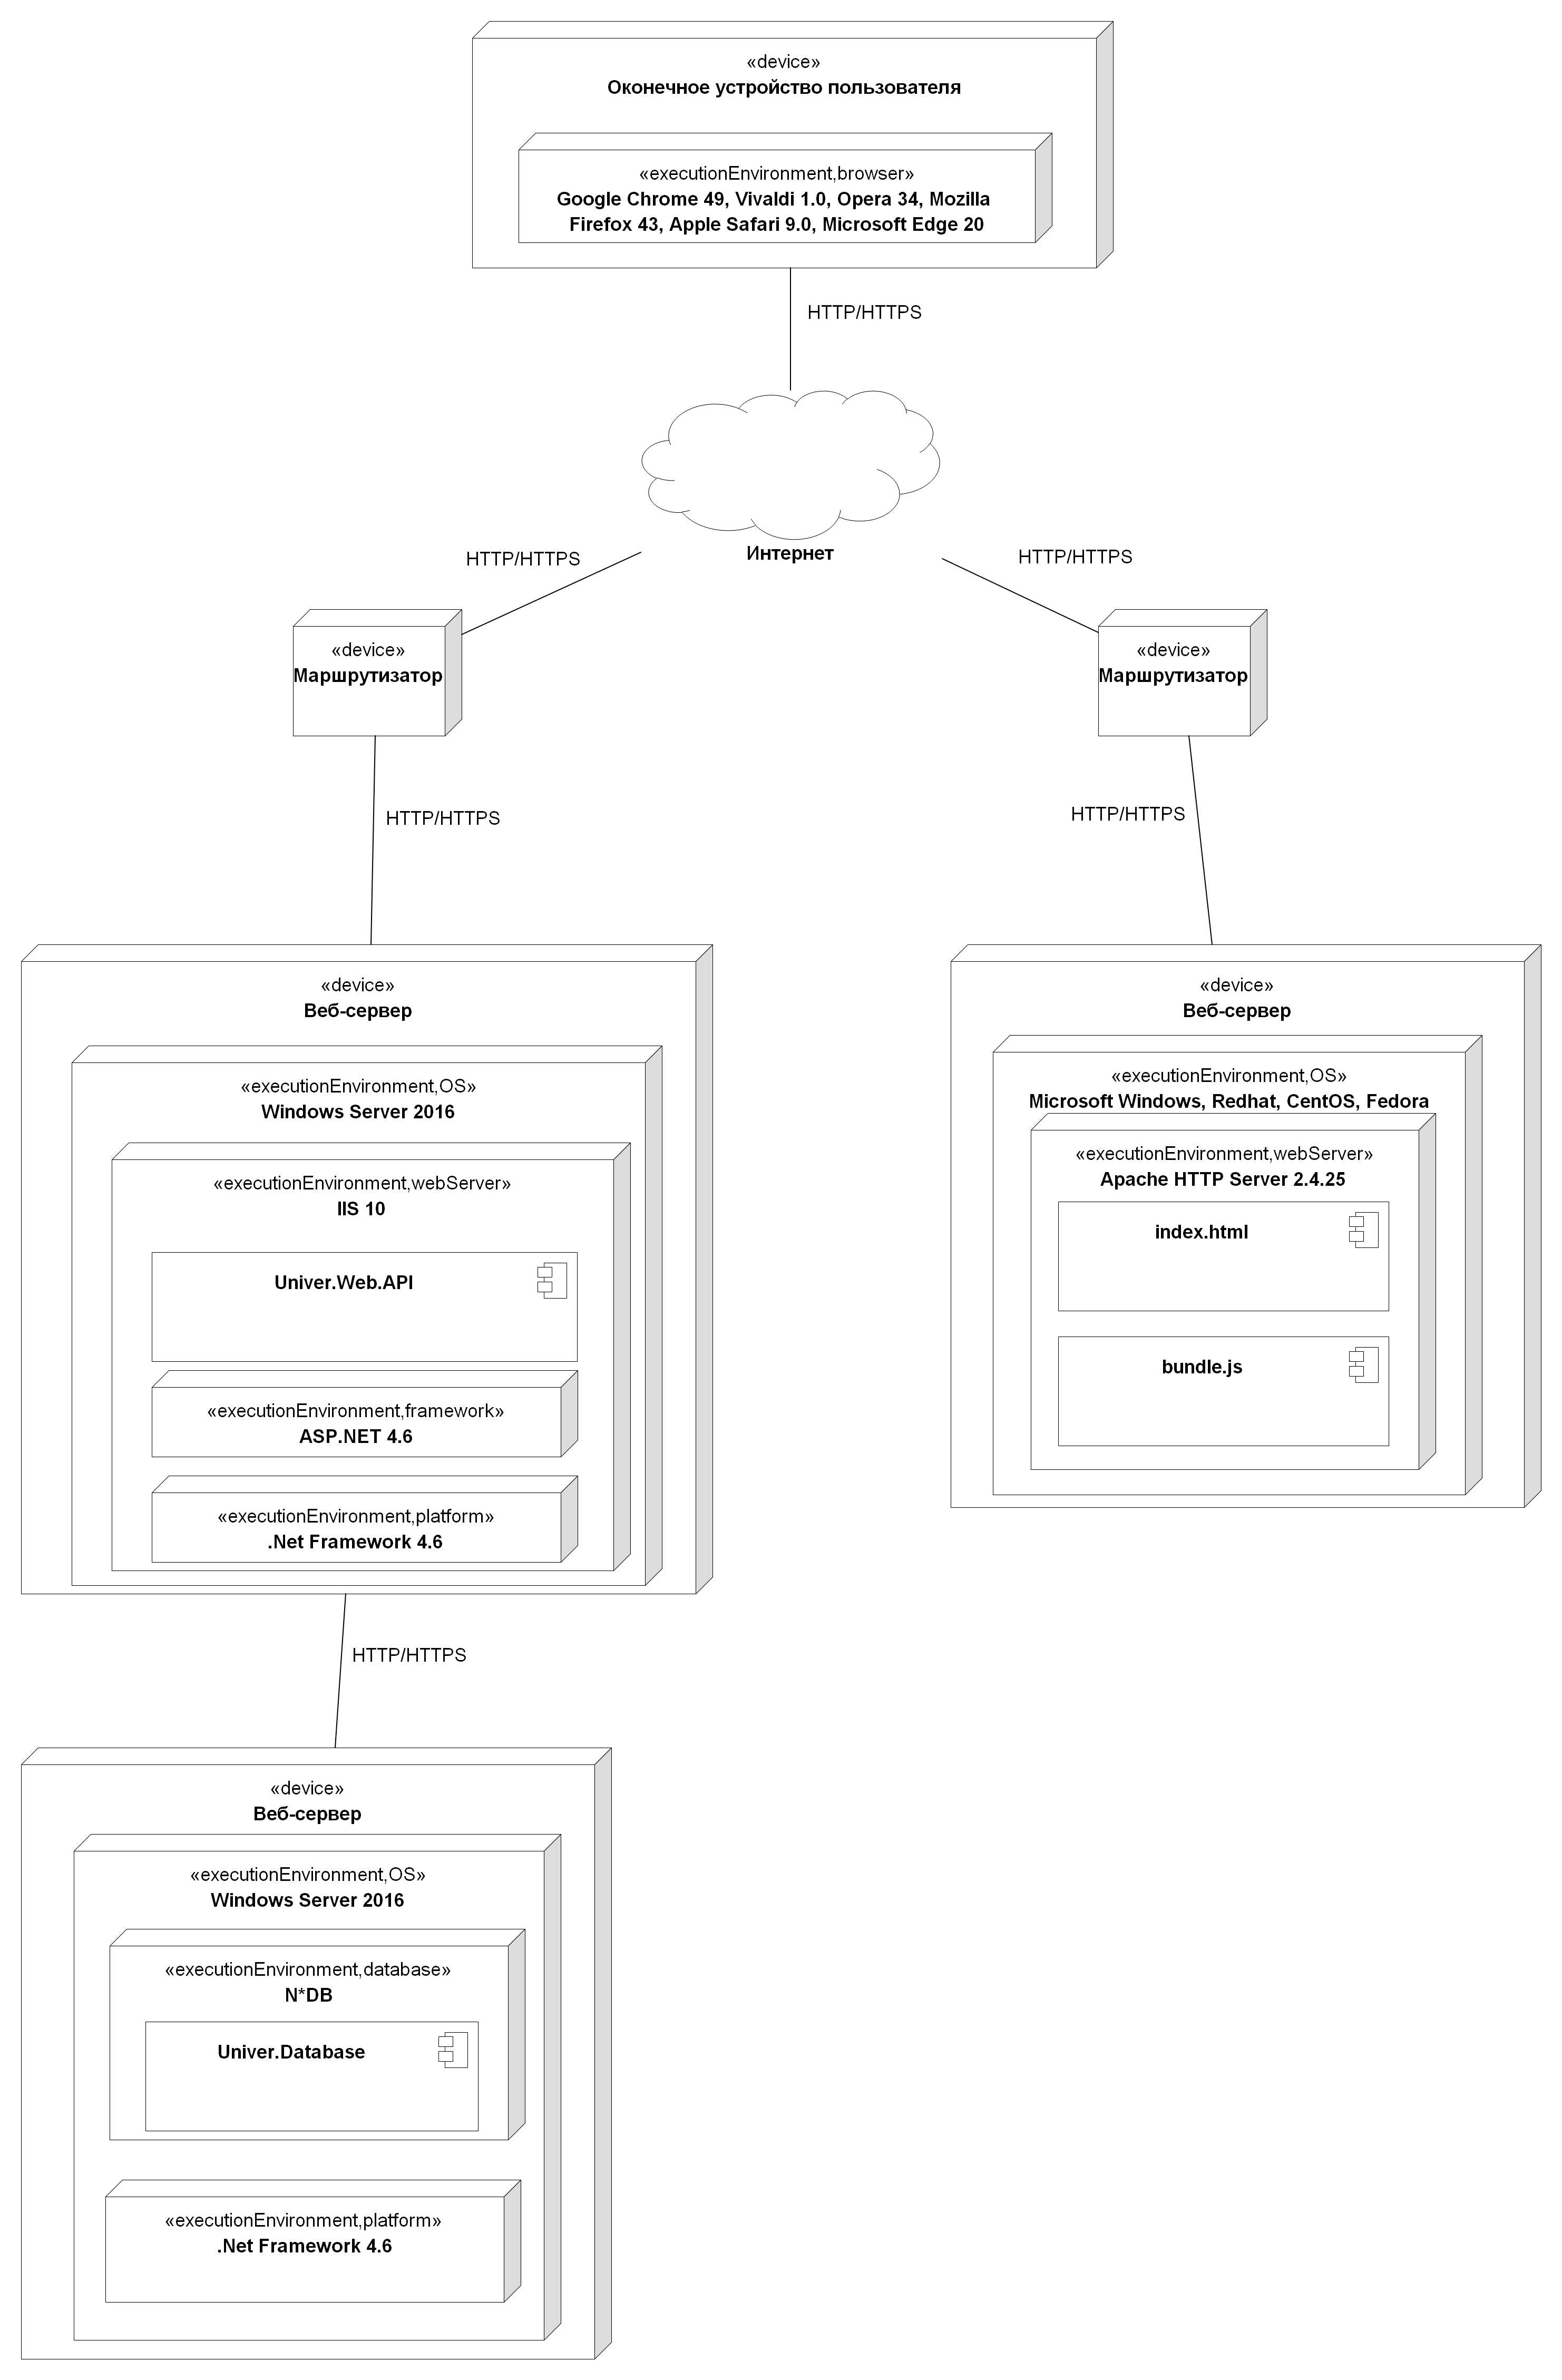
\includegraphics[scale=0.13]{deployment_diagram.png}
	\caption{Диаграмма развертывания ПС}
	\label{fig:design:deployment:diagram}
\end{figure}

Данная диаграмма представлена на рисунке~\ref{fig:design:deployment:diagram}. Она отражает следующие особенности развертывания:

\begin{itemize}
	\item На узле оконечного устройства в качестве среды выполнения перечислен список браузерных программных средств, с помощью которых можно использовать клиентскую часть приложения.
	\item В качестве операционной системы для сервера клиентской части перечислен список поддерживаемых веб-сервером ОС.
	\item При необходимости Apache HTTP Server может быть заменен другим HTTP-сервером.
	\item Для серверной части программного средства и базы данных показано их развертывание на отдельных узлах. При самом развертывании в зависимости от условий поставщика вычислительных мощностей данные элементы программной системы могут быть объединены на одном узле.
	\item В свою очередь, помимо упрощения, возможно и усложнение схемы развертывания, например, база данных будет развернута на нескольких узлах. Тем не менее, все узлы должны удовлетворять отображенным условиям.
	\item Все серверы: и клиентской части, и серверной, и базы данных, -- могут быть физически расположены в различных дата-центрах.
	\item Предполагается, что пользовательское оконечное устройство зна\-чи\-те\-льно удалено от серверов программной системы, доступ осуществляется через сеть Интернет, что и упрощенно показано на диаграмме.
\end{itemize}

Таким образом, после развертывания программного средства пользователи могут уже начать им пользоваться.


\subsection{Методика использования мобильного приложения}
\label{sec:manual}

В данном разделе приведены основные сведения по работе с мобильным приложением. 
Приложение доступно в AppStore и Android Market.
Рассмотрим основные функции, предоставляемые приложением пользователям.

При запуске приложение появляется экран с регистрацией/авторизацией (рисунок~\ref{fig:manual:login}).
Если пользователь забыл пароль, то он может его изменить, нажав на
соответствующую кнопку.

\begin{figure}[H]
\centering
	
\includegraphics[scale=0.6]{manual/login-screen.png}
	\caption{Экран авторизации}
	\label{fig:manual:login}
\end{figure}

Пользователь может зарегистрироваться с помощью номера телефона и
пароля, либо с помощью учётных данных от социальных сетей «Вконтакте»
или Facebook (рисунок ~\ref{fig:manual:auth}).

\begin{figure}[H]
  \centering
    
\includegraphics[scale=0.5]{manual/facebook-screen.png}
    \caption{Авторизация/вход через Facebook}
    \label{fig:manual:auth}
  \end{figure}

Профиль пользователя представлен на рисунке~\ref{fig:manual:profile}.

\begin{figure}[H]
  \centering
    
\includegraphics[scale=0.6]{manual/profile-screen.png}
    \caption{Профиль пользователя}
    \label{fig:manual:profile}
  \end{figure}

После нажатия кнопки «Применить» появляется страница, где
пользователь может увидеть фотографию (рисунок~\ref{fig:manual:creatingPost}), добавить к ней
комментарии, которые могут включать хештеги для облегчения поиска постов
по соответствующей тематике.

\begin{figure}[H]
    \centering
      
\includegraphics[scale=0.6]{manual/creating-post.png}
      \caption{Создание поста}
      \label{fig:manual:creatingPost}
\end{figure}

После нажатия кнопки «Сохранить» пост появляется в ленте (рисунок~\ref{fig:manual:uploadedPost}). Друзья смогут увидеть вашу запись, написать комментарий к ней и
лайкнуть.

\begin{figure}[H]
  \centering
    
\includegraphics[scale=0.6]{manual/uploaded-post.png}
    \caption{Лента пользователя с добавленной записью}
    \label{fig:manual:uploadedPost}
\end{figure}

Процесс загрузки фото и видео точно такой же, как и при добавлении
постов в ленту пользователя. После нажатия кнопки сохранить появляется
обновлённый гараж с записью о мотоцикле (рисунок~\ref{fig:manual:bike}).

\begin{figure}[H]
  \centering
    
\includegraphics[scale=0.6]{manual/bike.png}
    \caption{Гараж}
    \label{fig:manual:bike}
\end{figure}

Пользователь может принять запрос, просмотреть профиль
пользователя либо игнорировать его, в этом случае он останется в
подписчиках. При нажатии пункта добавить в друзья обновляется счётчик
друзей в профиле, и вы можете вести переписку (рисунок~\ref{fig:manual:dialog}).

\begin{figure}[H]
  \centering
    
\includegraphics[scale=0.6]{manual/dialog.png}
    \caption{Переписка}
    \label{fig:manual:dialog}
\end{figure}

Карта местности с метками друзей, кнопкой получения текущего
расположения, и установки меток представлена на рисунке\ref{fig:manual:map}.

\begin{figure}[H]
  \centering
    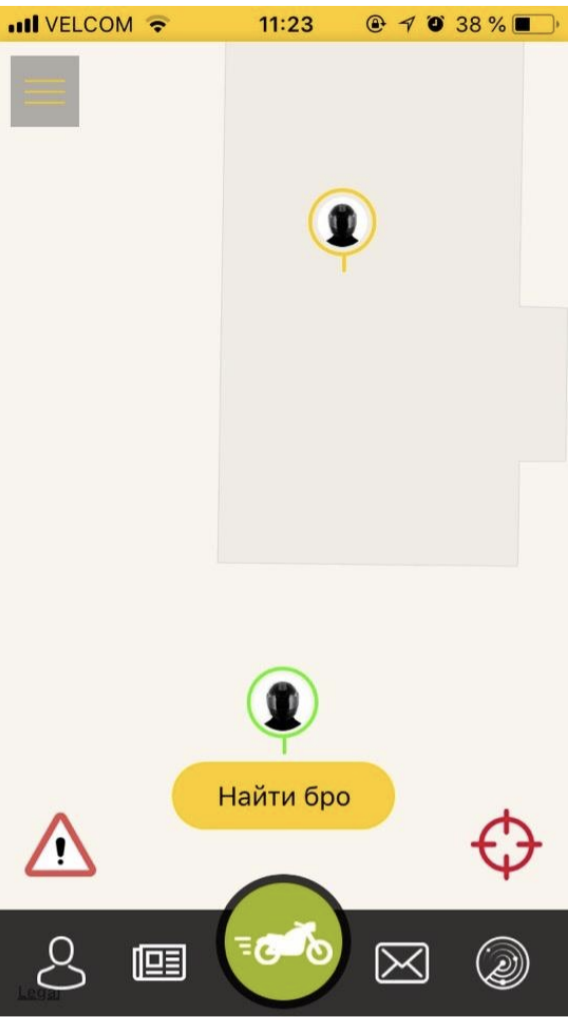
\includegraphics[scale=0.6]{manual/map.png}
    \caption{Карта}
    \label{fig:manual:map}
\end{figure}


Таким образом, в данном разделе приведены примеры использования некоторых их основных возможностей разработанного программного средства.



	% \input{sections/04_testing}

	\section{Методика использования программного средства}
\label{sec:manual}

В данном разделе приведены основные сведения по работе с программным средством. 
Приложение доступно в AppStore и Android Market.
Рассмотрим основные функции, предоставляемые приложением пользователям.

При запуске приложение появляется экран с регистрацией/авторизацией (рисунок~\ref{fig:manual:login}).
Если пользователь забыл пароль, то он может его изменить, нажав на
соответствующую кнопку.

\begin{figure}[H]
\centering
	
\includegraphics[scale=0.6]{manual/login-screen.png}
	\caption{Экран авторизации}
	\label{fig:manual:login}
\end{figure}

Пользователь может зарегистрироваться с помощью номера телефона и
пароля, либо с помощью учётных данных от социальных сетей «Вконтакте»
или Facebook (рисунок ~\ref{fig:manual:auth}).

\begin{figure}[H]
  \centering
    
\includegraphics[scale=0.5]{manual/facebook-screen.png}
    \caption{Авторизация/вход через Facebook}
    \label{fig:manual:auth}
  \end{figure}

Профиль пользователя представлен на рисунке~\ref{fig:manual:profile}.

\begin{figure}[H]
  \centering
    
\includegraphics[scale=0.6]{manual/profile-screen.png}
    \caption{Профиль пользователя}
    \label{fig:manual:profile}
  \end{figure}

После нажатия кнопки «Применить» появляется страница, где
пользователь может увидеть фотографию (рисунок~\ref{fig:manual:creatingPost}), добавить к ней
комментарии, которые могут включать хештеги для облегчения поиска постов
по соответствующей тематике.

\begin{figure}[H]
    \centering
      
\includegraphics[scale=0.6]{manual/creating-post.png}
      \caption{Создание поста}
      \label{fig:manual:creatingPost}
\end{figure}

После нажатия кнопки «Сохранить» пост появляется в ленте (рисунок~\ref{fig:manual:uploadedPost}). Друзья смогут увидеть вашу запись, написать комментарий к ней и
лайкнуть.

\begin{figure}[H]
  \centering
    
\includegraphics[scale=0.6]{manual/uploaded-post.png}
    \caption{Лента пользователя с добавленной записью}
    \label{fig:manual:uploadedPost}
\end{figure}

Процесс загрузки фото и видео точно такой же, как и при добавлении
постов в ленту пользователя. После нажатия кнопки сохранить появляется
обновлённый гараж с записью о мотоцикле (рисунок~\ref{fig:manual:bike}).

\begin{figure}[H]
  \centering
    
\includegraphics[scale=0.6]{manual/bike.png}
    \caption{Гараж}
    \label{fig:manual:bike}
\end{figure}

Пользователь может принять запрос, просмотреть профиль
пользователя либо игнорировать его, в этом случае он останется в
подписчиках. При нажатии пункта добавить в друзья обновляется счётчик
друзей в профиле, и вы можете вести переписку (рисунок~\ref{fig:manual:dialog}).

\begin{figure}[H]
  \centering
    
\includegraphics[scale=0.6]{manual/dialog.png}
    \caption{Переписка}
    \label{fig:manual:dialog}
\end{figure}

Карта местности с метками друзей, кнопкой получения текущего
расположения, и установки меток представлена на рисунке\ref{fig:manual:map}.

\begin{figure}[H]
  \centering
    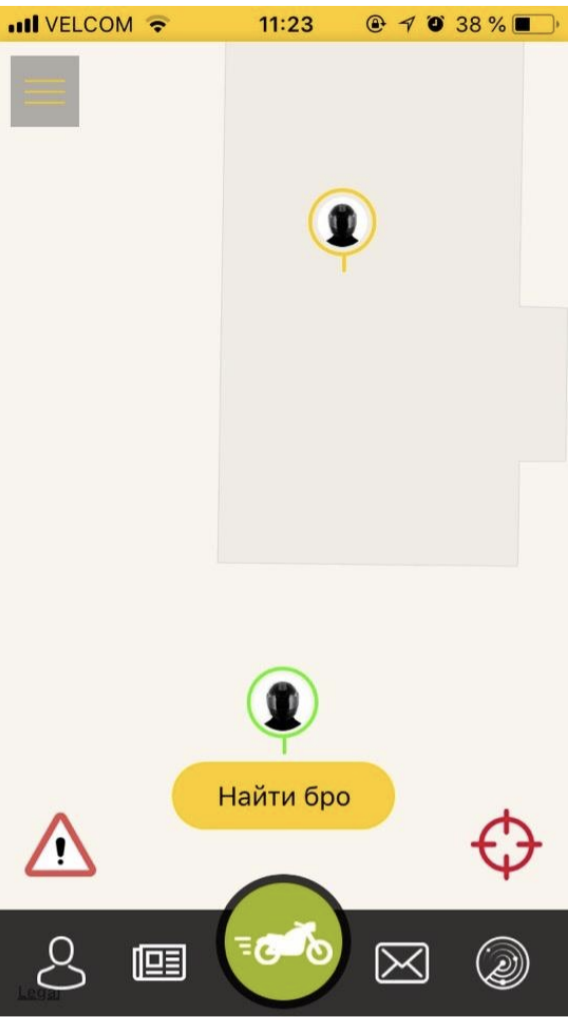
\includegraphics[scale=0.6]{manual/map.png}
    \caption{Карта}
    \label{fig:manual:map}
\end{figure}


Таким образом, в данном разделе приведены примеры использования некоторых их основных возможностей разработанного программного средства.


	\newcommand{\byn}{\text{руб.}}
\newcommand{\manhour}{\text{чел./ч.}}

\newcommand{\totalloc}{\text{V}_\text{о}}
\newcommand{\normativelaboriousness}{\text{Т}_\text{н}}
\newcommand{\complexity}{\text{К}_\text{с}}
\newcommand{\stdmodules}{\text{К}_\text{т}}
\newcommand{\novelty}{\text{К}_\text{н}}
\newcommand{\totallaboriousness}{\text{Т}_\text{о}}

\newcommand{\effectivetimefund}{\text{Ф}_\text{эф}}
\newcommand{\daysinyear}{\text{Д}_\text{г}}
\newcommand{\holidays}{\text{Д}_\text{п}}
\newcommand{\weekends}{\text{Д}_\text{в}}
\newcommand{\vacationdays}{\text{Д}_\text{о}}

\newcommand{\developersnumber}{\text{Ч}_\text{р}}
\newcommand{\developmenttime}{\text{Т}_\text{р}}
\newcommand{\developertimefundsymbol}{\text{Ф}_\text{пi}}

\newcommand{\firstratetariffsymbol}{\text{Т}_\text{ч}^1}
\newcommand{\averagehourspermonthsymbol}{\text{Ф}_\text{р}}
\newcommand{\hourspershiftsymbol}{\text{Т}_\text{ч}}
\newcommand{\bonusratesymbol}{K}

\newcommand{\basewagesymbol}{\text{З}_\text{о}}
\newcommand{\additionalwageratesymbol}{\text{Н}_\text{д}}
\newcommand{\additionalwagesymbol}{\text{З}_\text{д}}

\newcommand{\onecopyprofit}{\text{П}_\text{ед}}

\newcommand{\ssfratesymbol}{\text{Н}_\text{сз}}
\newcommand{\ssfchargessymbol}{\text{З}_\text{сз}}
\newcommand{\insuranceratesymbol}{\text{Н}_\text{ос}}
\newcommand{\insurancechargessymbol}{\text{З}_\text{ос}}

\newcommand{\consumablesratesymbol}{\text{Н}_\text{мз}}
\newcommand{\consumableschargessymbol}{\text{М}}

\newcommand{\machinetimeratesymbol}{\text{Н}_\text{мв}}
\newcommand{\machinehourpricesymbol}{\text{Ц}_\text{м}}
\newcommand{\machinetimechargessymbol}{\text{Р}_\text{м}}

\newcommand{\businesstripratesymbol}{\text{Н}_\text{рнк}}
\newcommand{\businesstripchargessymbol}{\text{Р}_\text{нк}}

\newcommand{\otherchargesratesymbol}{\text{Н}_\text{пз}}
\newcommand{\otherchargessymbol}{\text{П}_\text{з}}

\newcommand{\overheadratesymbol}{\text{Н}_\text{нр}}
\newcommand{\overheadchargessymbol}{\text{Р}_\text{н}}

\newcommand{\totalchargessymbol}{\text{С}_\text{п}}

\newcommand{\profitabilityratesymbol}{\text{У}_\text{рп}}
\newcommand{\profitabilitysymbol}{\text{П}_\text{о}}
\newcommand{\netprofitabilitysymbol}{\text{П}_\text{ч}}

\newcommand{\netpricesymbol}{\text{Ц}_\text{п}}

\newcommand{\vatsymbol}{\text{НДС}}
\newcommand{\vatsymbola}{\text{НДС}}
\newcommand{\vatratesymbol}{\text{Н}_\text{ДС}}

\newcommand{\sellingpricesymbol}{\text{Ц}_\text{о}}

\newcommand{\deploymentchargessymbol}{\text{Р}_\text{о}}
\newcommand{\deploymentratesymbol}{\text{Н}_\text{о}}
\newcommand{\maintenancechargessymbol}{\text{Р}_\text{с}}
\newcommand{\maintenanceratesymbol}{\text{Н}_\text{с}}

\newcommand{\capitalinvestmentsymbol}{\text{К}_\text{о}}
\newcommand{\purchasecostsymbol}{\text{К}_\text{пр}}
\newcommand{\deploymentcostsymbol}{\text{К}_\text{ос}}
\newcommand{\maintenancecostsymbol}{\text{К}_\text{с}}
\newcommand{\equipmentcostsymbol}{\text{К}_\text{тс}}
\newcommand{\assetscostsymbol}{\text{К}_\text{об}}

\newcommand{\averagewagesymbol}{\text{З}_\text{см}}
\newcommand{\baselabourisnesssymbol}{\text{Т}_\text{с1}}
\newcommand{\newlabourisnesssymbol}{\text{Т}_\text{с2}}
\newcommand{\basetaskscountsymbol}{\text{A}_\text{1}}
\newcommand{\newtaskscountsymbol}{\text{A}_\text{2}}

\newcommand{\wageeconomypertasksymbol}{\text{С}_\text{зе}}
\newcommand{\wageeconomysymbol}{\text{С}_\text{з}}
\newcommand{\totalwageeconomysymbol}{\text{С}_\text{н}}

\newcommand{\basedowntimesymbol}{\text{П}_\text{1}}
\newcommand{\newdowntimesymbol}{\text{П}_\text{2}}
\newcommand{\downtimepricesymbol}{\text{С}_\text{п}}
\newcommand{\downtimechargessymbol}{\text{С}_\text{с}}
\newcommand{\planserviceworktimesymbol}{\text{Д}_\text{рг}}

\newcommand{\totaleconomysymbol}{\text{С}_\text{о}}

\newcommand{\usernetprofitsymbol}{\text{П}_\text{ч}}
\newcommand{\profittaxratesymbol}{\text{Н}_\text{п}}

\newcommand{\countcopyssymbol}{\text{N}}

\newcommand{\sumprofitperyearsymbol}{\text{П}}

\newcommand{\clearProfitSymol}{\text{ЧП}}
\newcommand{\incomTaxRateSymbol}{\text{Н}_\text{п}}
\newcommand{\discontKSymbol}{\text{\(\alpha\)}_\text{i}}
\FPeval{\totalProgramSize}{17944}

\FPeval{\normativeManDays}{520}

\FPeval{\additionalComplexity}{clip(0.06+0.07)}

\FPeval{\stdModuleUsageFactor}{0.7}
\FPeval{\noveltyFactor}{0.9}

\FPeval{\daysInYear}{365}
\FPeval{\redLettersDaysInYear}{9}
\FPeval{\weekendDaysInYear}{103}
\FPeval{\vacationDaysInYear}{21}

\FPeval{\firstratetariff}{150}
\FPeval{\averagehourspermonth}{167.3}
\FPeval{\hourspershift}{8}
\FPeval{\bonusrate}{1.3}
\FPeval{\additionalwagerate}{20}
\FPeval{\ssfrate}{34}
\FPeval{\insurancerate}{0.6}
\FPeval{\consumablesrate}{5}
\FPeval{\machinetimerate}{15}
\FPeval{\machinetimereductionrate}{0.5}
\FPeval{\machinehourprice}{0.8}
\FPeval{\businesstriprate}{15}
\FPeval{\otherchargesrate}{18}
\FPeval{\overheadrate}{45}
\FPeval{\oneCopyPrice}{7}

\FPeval{\countfirstyearcopys}{1000}
\FPeval{\countsecondyearcopys}{1500}
\FPeval{\countthirdyearcopys}{2100}
\FPeval{\counfoursyearcopys}{3000}
\FPeval{\incomTaxRate}{0.18}

\FPeval{\profitabilityrate}{10}
\FPeval{\vatrate}{20}

\FPeval{\deploymentrate}{10}
\FPeval{\maintenancerate}{20}

\FPeval{\averagewage}{716.5}
\FPeval{\baselabourisness}{2}
\FPeval{\newlabourisness}{0.1}
\FPeval{\usesperday}{4}

\FPeval{\basedowntime}{50}
\FPeval{\newdowntime}{10}
\FPeval{\downtimeprice}{79.8}
\FPeval{\planserviceworktime}{300}

\FPeval{\profittaxrate}{18}
\FPeval{\refinancingTax}{0.1}



\FPeval{\totalProgramSizeCorrected}{\totalProgramSize}
\newcommand{\totallocfactor}{\num{\totalProgramSizeCorrected}}

\newcommand{\additionalcomplexityfactor}{\num{\additionalComplexity}}
\FPeval{\complexityFactor}{clip(1 + \additionalComplexity)}
\newcommand{\complexityfactor}{\num{\complexityFactor}}

\newcommand{\stdmodulesfactor}{\num{\stdModuleUsageFactor}}
\newcommand{\noveltyfactor}{\num{\noveltyFactor}}

\FPeval{\adjustedManDaysExact}{clip( \normativeManDays * \complexityFactor * \stdModuleUsageFactor * \noveltyFactor )}
\FPround{\adjustedManDays}{\adjustedManDaysExact}{0}
\newcommand{\normativelaboriousnessfactor}{\num{\normativeManDays}}
\newcommand{\totallaboriousnessfactor}{\num{\adjustedManDays}}


\FPeval{\workingDaysInYear}{ clip( \daysInYear - \redLettersDaysInYear - \weekendDaysInYear - \vacationDaysInYear ) }
\newcommand{\daysinyearfactor}{\num{\daysInYear}}
\newcommand{\holidaysfactor}{\num{\redLettersDaysInYear}}
\newcommand{\weekendsfactor}{\num{\weekendDaysInYear}}
\newcommand{\vacationdaysfactor}{\num{\vacationDaysInYear}}
\newcommand{\effectivetimefundfactor}{\num{\workingDaysInYear}}

\FPeval{\requiredNumberOfProgrammers}{3}
\newcommand{\developersnumberfactor}{\num{\requiredNumberOfProgrammers}}
\FPeval{\developmentTimeYearsExact}{\adjustedManDays / (\requiredNumberOfProgrammers * \workingDaysInYear)}
\FPround{\developmentTimeYears}{\developmentTimeYearsExact}{2}
\newcommand{\developmenttimeyearsfactor}{\num{\developmentTimeYears}}
\FPeval{\developmentTimeMonthsExact}{\developmentTimeYearsExact * 12}
\FPround{\developmentTimeMonths}{\developmentTimeMonthsExact}{1}
\newcommand{\developmenttimemonthsfactor}{\num{\developmentTimeMonths}}
\FPeval{\developmentTimeDaysExact}{\developmentTimeYearsExact * \daysInYear}
\FPround{\developmentTimeDays}{\developmentTimeDaysExact}{0}
\newcommand{\developmenttimefactor}{\num{\developmentTimeDays}}

\FPeval{\developertimefund}{round(\developmentTimeDays / \requiredNumberOfProgrammers,0)}
\newcommand{\developertimefundvalue}{\num{\developertimefund}}

\FPeval{\employeeAMonthExact}{\firstratetariff * 3.98}
\FPeval{\employeeBMonthExact}{\firstratetariff * 3.48}
\FPeval{\employeeCMonthExact}{\firstratetariff * 2.65}
\FPeval{\employeeAHourExact}{\employeeAMonthExact / \averagehourspermonth}
\FPeval{\employeeBHourExact}{\employeeBMonthExact / \averagehourspermonth}
\FPeval{\employeeCHourExact}{\employeeCMonthExact / \averagehourspermonth}
\FPround{\employeeAMonth}{\employeeAMonthExact}{2}
\FPround{\employeeBMonth}{\employeeBMonthExact}{2}
\FPround{\employeeCMonth}{\employeeCMonthExact}{2}
\FPround{\employeeAHour}{\employeeAHourExact}{2}
\FPround{\employeeBHour}{\employeeBHourExact}{2}
\FPround{\employeeCHour}{\employeeCHourExact}{2}
\newcommand{\employeeamonthwage}{\num{\employeeAMonth}}
\newcommand{\employeebmonthwage}{\num{\employeeBMonth}}
\newcommand{\employeecmonthwage}{\num{\employeeCMonth}}
\newcommand{\employeeahourwage}{\num{\employeeAHour}}
\newcommand{\employeebhourwage}{\num{\employeeBHour}}
\newcommand{\employeechourwage}{\num{\employeeCHour}}

\newcommand{\firstratetariffvalue}{\num{\firstratetariff}}
\newcommand{\averagehourspermonthvalue}{\num{\averagehourspermonth}}
\newcommand{\hourspershiftvalue}{\num{\hourspershift}}
\newcommand{\bonusratevalue}{\num{\bonusrate}}

\FPeval{\basewageExact}{(\employeeBHour + \employeeCHour) * \hourspershift * \developertimefund * \bonusrate}
\FPround{\basewage}{\basewageExact}{2}
\newcommand{\basewagevalue}{\num{\basewage}}

\newcommand{\additionalwageratevalue}{\num{\additionalwagerate}\%}
\FPeval{\additionalwage}{round(\basewage * \additionalwagerate / 100, 2)}
\newcommand{\additionalwagevalue}{\num{\additionalwage}}

\FPeval{\ssfcharges}{round((\basewage + \additionalwage) * \ssfrate / 100, 2)}
\FPeval{\insurancecharges}{round((\basewage + \additionalwage) * \insurancerate / 100, 2)}
\newcommand{\ssfchargesvalue}{\num{\ssfcharges}}
\newcommand{\ssfratevalue}{\num{\ssfrate}\%}
\newcommand{\insurancechargesvalue}{\num{\insurancecharges}}
\newcommand{\insuranceratevalue}{\num{\insurancerate}\%}

\FPeval{\consumablescharges}{round(\basewage * \consumablesrate / 100, 2)}
\newcommand{\consumablesratevalue}{\num{\consumablesrate}\%}
\newcommand{\consumableschargesvalue}{\num{\consumablescharges}}

\FPeval{\machinetimecharges}{round(\machinehourprice * \totalProgramSize / 100 * \machinetimerate * \machinetimereductionrate, 2)}
\newcommand{\machinetimechargesvalue}{\num{\machinetimecharges}}
\newcommand{\machinetimeratevalue}{\num{\machinetimerate}\%}
\newcommand{\machinetimereductionratevalue}{\num{\machinetimereductionrate}}
\newcommand{\machinehourpricevalue}{\num{\machinehourprice}}

\FPeval{\businesstripcharges}{round(\basewage * \businesstriprate / 100, 2)}
\newcommand{\businesstripratevalue}{\num{\businesstriprate}\%}
\newcommand{\businesstripchargesvalue}{\num{\businesstripcharges}}

\FPeval{\othercharges}{round(\basewage * \otherchargesrate / 100, 2)}
\newcommand{\otherchargesratevalue}{\num{\otherchargesrate}\%}
\newcommand{\otherchargesvalue}{\num{\othercharges}}

\FPeval{\overheadcharges}{round(\basewage * \overheadrate / 100, 2)}
\newcommand{\overheadratevalue}{\num{\overheadrate}\%}
\newcommand{\overheadvalue}{\num{\overheadcharges}}

\FPeval{\totalcharges}{\basewage + \additionalwage + \ssfcharges + \insurancecharges + \consumablescharges + \machinetimecharges + \businesstripcharges + \othercharges + \overheadcharges}
\FPeval{\totalchargesclipped}{clip(\totalcharges)}
\newcommand{\totalchargesvalue}{\num{\totalchargesclipped}}

\FPeval{\profitability}{round(\totalcharges * \profitabilityrate / 100, 2)}
\newcommand{\profitabilityratevalue}{\num{\profitabilityrate}\%}
\newcommand{\profitabilityvalue}{\num{\profitability}}

\FPeval{\netprice}{clip(\totalcharges + \profitability)}
\newcommand{\netpricevalue}{\num{\netprice}}

\FPeval{\vat}{round(\netprice * \vatrate / 100, 2)}
\newcommand{\vatvalue}{\num{\vat}}
\newcommand{\vatratevalue}{\num{\vatrate}\%}

\FPeval{\sellingprice}{clip(\netprice + \vat)}
\newcommand{\sellingpricevalue}{\num{\sellingprice}}

\FPeval{\vatsymbolaeval}{round((\oneCopyPrice * \vatrate) / (100 + \vatrate), 2)}
\newcommand{\vatsymbolavalue}{\num{\vatsymbolaeval}}

\FPeval{\countcopys}{clip(\countfirstyearcopys + \countsecondyearcopys + \countthirdyearcopys + \counfoursyearcopys)}

\FPeval{\onecopyprofiteval}{round(\oneCopyPrice - \vatsymbolaeval - (\sellingprice / \countcopys), 2)}
\newcommand{\onecopyprofitvalue}{\num{\onecopyprofiteval}}
%-----------------
\FPeval{\profitperyearvalueoneeval}{clip(\onecopyprofiteval * \countfirstyearcopys)}
\newcommand{\profitperyearvalueone}{\num{\profitperyearvalueoneeval}}
\FPeval{\profitperyearvaluetwoeval}{clip(\onecopyprofiteval * \countsecondyearcopys)}
\newcommand{\profitperyearvaluetwo}{\num{\profitperyearvaluetwoeval}}
\FPeval{\profitperyearvaluethreeeval}{clip(\onecopyprofiteval * \countthirdyearcopys)}
\newcommand{\profitperyearvaluethree}{\num{\profitperyearvaluethreeeval}}
\FPeval{\profitperyearvaluefoureval}{clip(\onecopyprofiteval * \counfoursyearcopys)}
\newcommand{\profitperyearvaluefour}{\num{\profitperyearvaluefoureval}}
%-----------------
%-----------------
\FPeval{\clearProfitValueOneEval}{clip(\profitperyearvalueoneeval - \profitperyearvalueoneeval * \incomTaxRate)}
\newcommand{\clearProfitValueOne}{\num{\clearProfitValueOneEval}}
\FPeval{\clearProfitValueTwoEval}{clip(\profitperyearvaluetwoeval - \profitperyearvaluetwoeval * \incomTaxRate)}
\newcommand{\clearProfitValueTwo}{\num{\clearProfitValueTwoEval}}
\FPeval{\clearProfitValueThreeEval}{clip(\profitperyearvaluethreeeval - \profitperyearvaluethreeeval * \incomTaxRate)}
\newcommand{\clearProfitValueThree}{\num{\clearProfitValueThreeEval}}
\FPeval{\clearProfitValueFourEval}{clip(\profitperyearvaluefoureval - \profitperyearvaluefoureval * \incomTaxRate)}
\newcommand{\clearProfitValueFour}{\num{\clearProfitValueFourEval}}
%-----------------
%-----------------
\FPeval{\discontKValueOneEval}{round(pow(-1, 1.1), 2)}
\newcommand{\discontKValueOne}{\num{\discontKValueOneEval}}
\FPeval{\discontKValueTwoEval}{round(pow(-2, 1.1), 2)}
\newcommand{\discontKValueTwo}{\num{\discontKValueTwoEval}}
\FPeval{\discontKValueThreeEval}{round(pow(-3, 1.1), 2)}
\newcommand{\discontKValueThree}{\num{\discontKValueThreeEval}}
%-----------------

\FPeval{\deploymentcharges}{round(\totalcharges * \deploymentrate / 100, 2)}
\newcommand{\deploymentratevalue}{\num{\deploymentrate}\%}
\newcommand{\deploymentchargesvalue}{\num{\deploymentcharges}}

\FPeval{\maintenancecharges}{round(\totalcharges * \maintenancerate / 100, 2)}
\newcommand{\maintenanceratevalue}{\num{\maintenancerate}\%}
\newcommand{\maintenancechargesvalue}{\num{\maintenancecharges}}

\FPeval{\netprofitability}{round(\profitability * (100 - \profittaxrate) / 100, 2)}
\newcommand{\netprofitabilityvalue}{\num{\netprofitability}}

\FPeval{\capitalinvestment}{clip(\maintenancecharges + \deploymentcharges + \sellingprice)}
\newcommand{\capitalinvestmentvalue}{\num{\capitalinvestment}}

\FPeval{\wageeconomypertask}{round(\averagewage * (\baselabourisness - \newlabourisness) / \averagehourspermonth, 2)}
\newcommand{\wageeconomypertaskvalue}{\num{\wageeconomypertask}}
\newcommand{\averagewagevalue}{\num{\averagewage}}
\newcommand{\baselabourisnessvalue}{\num{\baselabourisness}}
\newcommand{\newlabourisnessvalue}{\num{\newlabourisness}}

\FPeval{\taskscount}{clip(\usesperday * \daysInYear)}
\newcommand{\taskscountvalue}{\num{\taskscount}}
\newcommand{\usesperdayvalue}{\num{\usesperday}}

\FPeval{\wageeconomy}{clip(\wageeconomypertask * \taskscount)}
\newcommand{\wageeconomyvalue}{\num{\wageeconomy}}

\FPeval{\totalwageeconomy}{round(\wageeconomy * (100 + \bonusrate) / 100,2)}
\newcommand{\totalwageeconomyvalue}{\num{\totalwageeconomy}}

\FPeval{\downtimecharges}{round((\basedowntime - \newdowntime) * \planserviceworktime * \downtimeprice / 60,2)}
\newcommand{\downtimechargesvalue}{\num{\downtimecharges}}
\newcommand{\basedowntimevalue}{\num{\basedowntime}}
\newcommand{\newdowntimevalue}{\num{\newdowntime}}
\newcommand{\downtimepricevalue}{\num{\downtimeprice}}
\newcommand{\planserviceworktimevalue}{\num{\planserviceworktime}}

\FPeval{\totaleconomy}{clip(\totalwageeconomy + \downtimecharges)}
\newcommand{\totaleconomyvalue}{\num{\totaleconomy}}

\FPeval{\usernetprofit}{round(\totaleconomy * (1 - \profittaxrate / 100),2)}
\newcommand{\profittaxratevalue}{\num{\profittaxrate}\%}
\newcommand{\usernetprofitvalue}{\num{\usernetprofit}}

\FPeval{\usernetprofityearone}{round(\usernetprofit * 0.8696,2)}
\newcommand{\usernetprofityearonevalue}{\num{\usernetprofityearone}}
\FPeval{\usernetprofityeartwo}{round(\usernetprofit * 0.7561,2)}
\newcommand{\usernetprofityeartwovalue}{\num{\usernetprofityeartwo}}
\FPeval{\usernetprofityearthree}{round(\usernetprofit * 0.6575,2)}
\newcommand{\usernetprofityearthreevalue}{\num{\usernetprofityearthree}}

\FPeval{\excessovercostsyearzero}{clip(-\capitalinvestment)}
\newcommand{\excessovercostsyearzerovalue}{\num{\excessovercostsyearzero}}
\FPeval{\excessovercostsyearone}{clip(\usernetprofityearone)}
\newcommand{\excessovercostsyearonevalue}{\num{\excessovercostsyearone}}
\FPeval{\excessovercostsyeartwo}{clip(\usernetprofityeartwo)}
\newcommand{\excessovercostsyeartwovalue}{\num{\excessovercostsyeartwo}}
\FPeval{\excessovercostsyearthree}{clip(\usernetprofityearthree)}
\newcommand{\excessovercostsyearthreevalue}{\num{\excessovercostsyearthree}}

\FPeval{\excessovercostswithtimingyearone}{clip(\excessovercostsyearzero + \usernetprofityearone)}
\newcommand{\excessovercostswithtimingyearonevalue}{\num{\excessovercostswithtimingyearone}}
\FPeval{\excessovercostswithtimingyeartwo}{clip(\excessovercostswithtimingyearone + \usernetprofityeartwo)}
\newcommand{\excessovercostswithtimingyeartwovalue}{\num{\excessovercostswithtimingyeartwo}}
\FPeval{\excessovercostswithtimingyearthree}{clip(\excessovercostswithtimingyeartwo + \usernetprofityearthree)}
\newcommand{\excessovercostswithtimingyearthreevalue}{\num{\excessovercostswithtimingyearthree}}


\section{Технико-экономическое обоснование разработки и внедрения программного средства}
\label{sec:economics}

\subsection{Характеристика программного средства}
\label{sec:economics:description}

% Программное средство, разрабатываемое в рамках дипломного проекта, предназначено для автоматизации основных задач участников учебного процесса университетов: управление расписанием, заданиями и коммуникацией. Существует большое число средств, с помощью которых могут решаться перечисленные задачи, однако данное многообразие приводит к разрозненности рабочих окружений разных людей. Вследствие ее возникновения у всех участников учебного процесса появляется необходимость в совершении рутинных действий по настройке своей рабочей среды. Кроме того, различия в используемых средствах приводят к необходимости дополнительных действий по сопряжению интерфейсов коммуникации. Данные проблемы могут быть решены путем создания системы, которая бы объединяла и унифицировала задачи управления событиями календаря, задачами и контактами.

% Разработки проектов программных средств связана со значительными затратами ресурсов. В связи с этим создание и реализация каждого проекта программного обеспечения нуждается в соответствующем тех\-ни\-ко-эко\-но\-ми\-чес\-ком обосновании~\cite{palitsyn}, которое и описывается в данном разделе.

\subsection{Расчет сметы затрат}
\label{sec:economics:estimate}

Основной статьей расходов на создание ПО является заработная плата разработчиков проекта. 
Затраты на основную зароботную плату команды разработчиков определяются исходя из состава и численности команды, размеров месячной заработной платы каждого из участников команды, а также общей трудоемкости разработки ПО.
Информация об исполнителях перечислена в таблице~\ref{table:economics:estimate:employees}. Кроме того, в ней приведены данные об их тарифных разрядах, приведены разрядные коэффициенты, а также по формулам~\ref{eq:economics:estimate:month_wage} и~\ref{eq:economics:estimate:hour_wage} рассчитаны месячный и часовой оклады.

\begin{table}[!hb]
  \caption{Работники, занятые в проекте}
  \label{table:economics:estimate:employees}
  \begin{tabular}{| >{\raggedright}m{0.3\textwidth} 
                  | >{\centering}m{0.09\textwidth} 
                  | >{\centering}m{0.18\textwidth} 
                  | >{\centering}m{0.15\textwidth} 
                  | >{\centering\arraybackslash}m{0.15\textwidth}|}
	\hline
	{\begin{center}Исполнители\end{center}} & Разряд & Тарифный коэффициент & Месячный оклад, \byn & Часовой оклад, \byn \\

	\hline
	Руководитель проекта & 17 & \num{3.98} & \employeeamonthwage & \employeeahourwage \\

	\hline
	Ведущий инженер-программист & 15 & \num{3.48} & \employeebmonthwage & \employeebhourwage\\

	\hline
	Инженер-программист II категории & 11 & \num{2.65} & \employeecmonthwage & \employeechourwage\\
	\hline
  \end{tabular}
\end{table}

\begin{equation}
\label{eq:economics:estimate:month_wage}
	\text{T}_\text{м} = \text{T}_\text{м}^1 \cdot \text{T}_\text{к},
\end{equation}
\begin{equation}
\label{eq:economics:estimate:hour_wage}
	\text{T}_\text{ч} = \frac{\text{T}_\text{м}}{\text{Ф}_\text{р}},
\end{equation}
\begin{explanation}
где & $ \text{T}_\text{м} $ & месячный оклад;\\
	& $ \text{T}_\text{м}^1 $ & тарифная ставка 1-го разряда (положим ее равной \num{\firstratetariff} \byn);\\
	& $ \text{T}_\text{к} $ & тарифный коэффициент;\\
	& $ \text{T}_\text{ч} $ & часовой оклад;\\
	& $ \text{Ф}_\text{р} $ & среднемесячная норма рабочего времени (в 2017 г. составляет \num{168.3} ч.~\cite{labour_calendar}).
\end{explanation}

Тогда основная заработная плата исполнителей составит
\begin{equation}
\begin{aligned}
	\basewagesymbol &= \sum_{i=1}^n \text{Т}_\text{чi} \cdot \text{Т}_\text{ч} \cdot \developertimefundsymbol \cdot K = \\
	&= (\employeeahourwage + \employeebhourwage + \employeechourwage) \cdot \hourspershiftvalue \cdot \developertimefundvalue \cdot \bonusratevalue = \basewagevalue~\text{\byn},
\end{aligned}
\end{equation}
\begin{explanation}
где & $ \text{Т}_\text{чi} $ & часовая тарифная ставка i-го исполнителя, \byn;\\
	& $ \text{Т}_\text{ч} $ & количество часов работы в день;\\
	& $ \text{Ф}_\text{пi} $ & плановый фонд рабочего времени i-го исполнителя, д.;\\
	& $ K $ & коэффициент премирования (принятый равным \bonusratevalue).
\end{explanation}

Дополнительная заработная плата включает выплаты, предусмотренные законодательство о труде: оплата отпусков, льготных часов, времени  выполнения  государственных обязанностей и других выплат, не связанных с основной деятельностью исполнителей, и определяется по нормативу, установленному в организации, в процентах к основной заработной плате.
Приняв данный норматив $\additionalwageratesymbol = \additionalwageratevalue$, рассчитаем дополнительные выплаты
\begin{equation}
	\additionalwagesymbol = \frac{\basewagesymbol \cdot \additionalwageratesymbol}{100\%} = \frac{\basewagevalue \cdot \additionalwageratevalue}{100\%} = \additionalwagevalue~\byn
\end{equation}

Отчисления в фонд социальной защиты населения и в фонд обязательного страхования определяются в соответствии с действующим законодательством по нормативу в процентном отношении к фонду основной и дополнительной зарплат по следующим формулам
\begin{equation}
\begin{aligned}
	\ssfchargessymbol &= \frac{(\basewagesymbol + \additionalwagesymbol) \cdot \ssfratesymbol}{100\%},\\
	\insurancechargessymbol &= \frac{(\basewagesymbol + \additionalwagesymbol) \cdot \insuranceratesymbol}{100\%}.
\end{aligned}
\end{equation} 

В настоящее время нормы отчислений в ФСЗН $\ssfratesymbol~=~\ssfratevalue$ и в фонд обязательного страхования $\insuranceratesymbol~=~\insuranceratevalue$. Исходя из этого, размеры отчислений
\begin{equation}
\begin{aligned}
	\ssfchargessymbol &= \frac{(\basewagevalue + \additionalwagevalue) \cdot \ssfratevalue}{100\%} = \ssfchargesvalue~\byn,\\[5mm]
	\insurancechargessymbol &= \frac{(\basewagevalue + \additionalwagevalue) \cdot \insuranceratevalue}{100\%} = \insurancechargesvalue~\byn\\[5mm]
\end{aligned}
\end{equation}

Расходы по статье <<Материалы>> отражают траты на магнитные носители, бумагу, красящие материалы, необходимые для разработки ПО определяются по нормативу к фонду основной заработной платы разработчиков. Исходя из принятого норматива $\consumablesratesymbol~=~\consumablesratevalue$ определим величину расходов

\begin{equation}
	\consumableschargessymbol = \frac{\basewagesymbol \cdot \consumablesratesymbol}{100\%} = \frac{\basewagevalue \cdot \consumablesratevalue}{100\%} = \consumableschargesvalue~\byn\\[5mm]
\end{equation}

Расходы по статье <<Машинное время>> включают оплату машинного времени, необходимого для разработки и отладки ПО, которое определяется по нормативам на 100 строк исходного кода. Норматив зависит от характера решаемых задач и типа ПК; для текущего проекта примем $\machinetimeratesymbol~=~\machinetimeratevalue$~\cite[приложение 6]{palitsyn}. Примем величину стоимости машино-часа $\machinehourpricesymbol~=~\machinehourpricevalue~\byn$ Тогда, применяя понижающий коэффициент \machinetimereductionratevalue, получим величину расходов
\begin{equation}
	\machinetimechargessymbol = \machinehourpricesymbol \cdot \frac{\totalloc}{100} \cdot \machinetimeratesymbol = \machinehourpricevalue \cdot \frac{\totallocfactor}{100} \cdot \machinetimeratevalue \cdot \machinetimereductionratevalue = \machinetimechargesvalue~\byn
\end{equation}

Расходы по статье <<Научные командировки>> определяются по нормативу в процентах к основной заработной плате. Принимая норматив равным $\businesstripratesymbol~=~\businesstripratevalue$ получим величину расходов
\begin{equation}
	\businesstripchargessymbol = \frac{\basewagesymbol \cdot \businesstripratesymbol}{100\%} = \frac{\basewagevalue \cdot \businesstripratevalue}{100\%} = \businesstripchargesvalue~\byn
\end{equation}

Расходы по статье <<Прочие затраты>> включают затраты на приобретение и подготовку специальной научно-технической информации и специальной литературы. Определяются по нормативу в процентах к основной заработной плате. Принимая норматив равным $\otherchargesratesymbol~=~\otherchargesratevalue$ получим величину расходов
\begin{equation}
	\otherchargessymbol = \frac{\basewagesymbol \cdot \otherchargesratesymbol}{100\%} = \frac{\basewagevalue \cdot \otherchargesratevalue}{100\%} = \otherchargesvalue~\byn
\end{equation}

Затраты по статье <<Накладные расходы>>, связанные с необходимостью  содержания  аппарата  управления,  вспомогательных хозяйств и опытных (экспериментальных) производств, а также с расходами на общехозяйственные нужды, относятся к конкретному ПО по нормативу в процентном отношении к основной заработной плате
исполнителей. Принимая норматив равным $\overheadratesymbol~=~\overheadratevalue$ получим величину расходов
\begin{equation}
	\overheadchargessymbol = \frac{\basewagesymbol \cdot \overheadratesymbol}{100\%} = \frac{\basewagevalue \cdot \overheadratevalue}{100\%} = \overheadvalue~\byn
\end{equation}

Общая сумма расходов по смете определяется как сумма вышерассчитанных показателей

\begin{equation}
\begin{aligned}
	\totalchargessymbol = \basewagesymbol + \additionalwagesymbol + \ssfchargessymbol &+ \insurancechargessymbol + \consumableschargessymbol + \machinetimechargessymbol + \businesstripchargessymbol + \otherchargessymbol + \overheadchargessymbol =\\
	&= \totalchargesvalue~\byn
\end{aligned}
\end{equation}

Рентабельность определяется из результатов анализа рыночных условий и переговоров с потребителями ПО. Исходя из принятого уровня рентабельности $\profitabilityratesymbol~=~\profitabilityratevalue$, прибыль от реализации ПО составит
\begin{equation}
	\profitabilitysymbol = \frac{\totalchargessymbol \cdot \profitabilityratesymbol}{100\%} = \frac{\totalchargesvalue \cdot \profitabilityratevalue}{100\%} = \profitabilityvalue~\byn
\end{equation}

На основании расчета прибыли и уровня себестоимости рассчитаем прогнозируемую цену программного средства без учета налогов
\begin{equation}
	\netpricesymbol = \totalchargessymbol + \profitabilitysymbol = \totalchargesvalue + \profitabilityvalue = \netpricevalue~\byn
\end{equation}

Далее рассчитаем налог на добавленную стоимость
\begin{equation}
	\vatsymbol = \frac{\netpricesymbol \cdot \vatratesymbol}{100\%} = \frac{\netpricevalue \cdot \vatratevalue}{100\%} = \vatvalue~\byn
\end{equation}

НДС включается в прогнозируемую отпускную цену
\begin{equation}
	\sellingpricesymbol = \netpricesymbol + \vatsymbol = \netpricevalue + \vatvalue = \sellingpricevalue~\byn
\end{equation}

Организация-разработчик участвует в освоении и внедрении ПО и несет соответствующие затраты, которые определяются по нормативу\linebreak $\deploymentratesymbol~=~\deploymentratevalue$ от себестоимости ПО в расчете на три месяца
\begin{equation}
	\deploymentchargessymbol = \frac{\totalchargessymbol \cdot \deploymentratesymbol}{100\%} = \frac{\totalchargesvalue \cdot \deploymentratevalue}{100\%} = \deploymentchargesvalue~\byn
\end{equation}

Кроме того, организация-разработчик осуществляет сопровождение\linebreak ПО, которое также оплачивается заказчиком. Расчет осуществляется в соответствии с нормативом $\maintenanceratesymbol~=~\maintenanceratevalue$ от себестоимости ПО
\begin{equation}
	\maintenancechargessymbol = \frac{\totalchargessymbol \cdot \maintenanceratesymbol}{100\%} = \frac{\totalchargesvalue \cdot \maintenanceratevalue}{100\%} = \maintenancechargesvalue~\byn
\end{equation}

Экономическим эффектом разработчика будет являться сумма прибыли с вычетом налога на прибыль
\begin{equation}
	\netprofitabilitysymbol = \profitabilitysymbol - \frac{\profitabilitysymbol \cdot \profittaxratesymbol}{100\%} = \profitabilityvalue - \frac{\profitabilityvalue \cdot \profittaxratevalue}{100\%} = \netprofitabilityvalue~\byn
\end{equation}

\subsection{Оценка экономической эффективности применения программного средства у пользователя}
\label{sec:economics:effect}

В результате применения нового ПО пользователь может понести значительные капитальные затраты на приобретение и освоение ПО, доукомплектованием ЭВМ новыми техническими средствами и пополнение оборотных средств. Однако, если приобретенное ПО будет в достаточной степени эффективнее базового, то дополнительные капитальные затраты быстро окупятся.

Для определения экономического эффекта от использования нового ПО у потребителя необходимо сравнить расходы по всем основным статьям сметы затрат на эксплуатацию нового ПО с расходами по соответствующим статьям базового варианта. При этом за базовый вариант примем ручной вариант. Исходные данные для расчета приведены в таблице~\ref{table:economics:effect:initial_data}. Размер средней зарплаты приведен на февраль 2017 г.

\begin{table}[!hb]
\caption{Исходные данные}
\label{table:economics:effect:initial_data}
\centering
	\begin{tabular}{{ 
	|>{\raggedright}m{0.4\textwidth} | 
	 >{\centering}m{0.17\textwidth} | 
	 >{\centering}m{0.14\textwidth} | 
	 >{\centering\arraybackslash}m{0.18\textwidth}|}}

  	\hline
	{\begin{center} Наименование показателя \end{center}} & Условное обозначение & Значение в базовом варианте & Значение в новом варианте \\

	\hline
	Затраты пользователя на приобретение ПО & $\purchasecostsymbol$ & --- & \sellingpricevalue~\byn\\

	\hline
	Затраты пользователя на освоение & $\deploymentcostsymbol$ & --- & \deploymentchargesvalue~\byn\\

	\hline
	Затраты пользователя на сопровождение & $\maintenancecostsymbol$ & --- & \maintenancechargesvalue~\byn\\

	\hline
	Трудоемкость на задачу,~\manhour & $\baselabourisnesssymbol,\newlabourisnesssymbol$ & \baselabourisnessvalue & \newlabourisnessvalue\\

	\hline
	Средняя зарплата,~\byn & $\averagewagesymbol$ & \averagewagevalue & \averagewagevalue\\

	\hline
	Количество выполняемых задач & $\basetaskscountsymbol,\newtaskscountsymbol$ & \taskscountvalue & \taskscountvalue\\

	\hline
	Время простоя сервиса, мин. в день & $\basedowntimesymbol,\newdowntimesymbol$ & \basedowntimevalue & \newdowntimevalue\\

	\hline
	Стоимость одного часа простоя, \byn & $\downtimepricesymbol$ & \downtimepricevalue & \downtimepricevalue\\

	\hline
	\end{tabular}
\end{table}

Общие капитальные вложения заказчика (потребителя) вычисляются следующим образом
\begin{equation}
\begin{aligned}
	\capitalinvestmentsymbol = \purchasecostsymbol + \deploymentcostsymbol + \maintenancecostsymbol &= \sellingpricevalue + \deploymentchargesvalue + \maintenancechargesvalue = \\
	&= \capitalinvestmentvalue~\byn
\end{aligned}
\end{equation}
\begin{explanation}
где &$ \purchasecostsymbol $& затраты пользователя на приобретение ПО по отпускной цене;\\
	&$ \deploymentcostsymbol $& затраты пользователя на освоение;\\
	&$ \maintenancecostsymbol $& затраты пользователя на оплату услуг по сопровождению.
\end{explanation}

В качестве типичного примера использования разрабатываемого ПС\linebreak предполагается сценарий ее использования ежедневно $\usesperday$ раза в день, при этом предполагается снижение трудоемкости с $\baselabourisnesssymbol~=~\baselabourisnessvalue~\manhour$ до\\ $\newlabourisnesssymbol~=~\newlabourisnessvalue~\manhour$. Приняв среднемесячную заработную плату работника\linebreak $\averagewagesymbol~=~\averagewagevalue~\byn$, рассчитаем экономию затрат на заработную плату в расчете на одну задачу $\wageeconomypertasksymbol$ и за год $\wageeconomysymbol$ 
\begin{equation}
	\wageeconomypertasksymbol = \frac{\averagewagesymbol \cdot (\baselabourisnesssymbol - \newlabourisnesssymbol)}{\averagehourspermonthsymbol} = \frac{\averagewagevalue \cdot (\baselabourisnessvalue - \newlabourisnessvalue)}{\averagehourspermonthvalue} = \wageeconomypertaskvalue~\byn,
\end{equation}
\begin{equation}
	\wageeconomysymbol = \wageeconomypertasksymbol \cdot \newtaskscountsymbol = \wageeconomypertaskvalue \cdot \taskscountvalue = \wageeconomyvalue~\byn,
\end{equation}
\begin{explanation}
где &$\averagehourspermonthsymbol$& среднемесячная норма рабочего времени, ч.
\end{explanation}

Экономия с учетом начислений на зарплату
\begin{equation}
	\totalwageeconomysymbol = \wageeconomysymbol \cdot \frac{100\% + \bonusratesymbol}{100\%} = \wageeconomyvalue \cdot \frac{100\% + \bonusratevalue}{100\%} = \totalwageeconomyvalue~\byn,
\end{equation}
\begin{explanation}
где &$\bonusratesymbol$& норматив начислений на зарплату, \byn
\end{explanation}

Экономия за счет сокращения простоев сервиса
\begin{equation}
	\downtimechargessymbol = \frac{(\basedowntimesymbol - \newdowntimesymbol) \cdot \planserviceworktimesymbol \cdot \downtimepricesymbol}{60} = \frac{(\basedowntimevalue - \newdowntimevalue) \cdot \planserviceworktimevalue \cdot \downtimepricevalue}{60} = \downtimechargesvalue,~\byn,
\end{equation}
\begin{explanation}
где &$\planserviceworktimesymbol$& плановый фонд работы сервиса, д.
\end{explanation}

Тогда общая годовая экономия текущих затрат, связанных с использованием нового ПО
\begin{equation}
	\totaleconomysymbol = \totalwageeconomysymbol + \downtimechargessymbol = \totalwageeconomyvalue + \downtimechargesvalue = \totaleconomyvalue~\byn
\end{equation}

Внедрение нового ПО позволит пользователю сэкономить на текущих затратах, то есть получить на эту сумму дополнительную прибыль. Для пользователя в качестве экономического эффекта выступает лишь чистая прибыль. Принимая размер ставки налога на прибыль $\profittaxratesymbol~=~\profittaxratevalue$ получим
\begin{equation}
	\Delta\usernetprofitsymbol = \totaleconomysymbol - \frac{\totaleconomysymbol \cdot \profittaxratesymbol}{100\%} = \totaleconomyvalue - \frac{\totaleconomyvalue \cdot \profittaxratevalue}{100\%} = \usernetprofitvalue~\byn
\end{equation}

В процессе использования нового ПО чистая прибыль в конечном итоге возмещает капитальные затраты. Однако полученные при этом суммы прибыли и затрат по годам приводят к единому времени -- расчетному году (за расчетный год принят 2017-й год) путем умножения результатов и затрат за каждый год на коэффициент дисконтирования $\alpha$. При расчете используются следующие коэффициенты: $2017~\text{г.} - \num{1}, 2018~\text{г.} - \num{0.8696}, 2019~\text{г.} - \num{0.7561}, 2020~\text{г.} - \num{0.6575}$. Все рассчитанные данные экономического эффекта сведены в таблицу~\ref{table:economics:effect:final_data}.

В результате технико-экономического обоснования применения ПС были получены следующие значения показателей эффективности:

\begin{itemize}
	\item чистая прибыль разработчика составит $\netprofitabilitysymbol~=~\netprofitabilityvalue~\byn$;
	\item затраты заказчика окупятся уже на четвертом году использования;
	\item экономическая эффективность для заказчика, выраженная в виде чистого дисконтированного дохода, составит $\excessovercostswithtimingyearthreevalue~\byn$ за четыре года использования данного ПС; более высокий прирост прибыли заказчик получит по истечению данного срока.
\end{itemize}

% \begin{longtable}{{|>{\raggedright}m{0.32\textwidth} | 
% 					>{\centering}m{0.1375\textwidth} | 
% 					>{\centering}m{0.1375\textwidth} | 
% 					>{\centering}m{0.1375\textwidth} | 
% 					>{\centering\arraybackslash}m{0.1375\textwidth}|}}
% \caption{Расчет экономического эффекта от использования нового ПО}
% \label{table:economics:effect:final_data}
% \centering

%   	\hline
% 	\begin{minipage}{1\linewidth}
% 		\centering Название показателя
% 	\end{minipage} & 
% 	\begin{minipage}{1\linewidth}
% 		\centering 2017 г.
% 	\end{minipage} & 
% 	\begin{minipage}{1\linewidth}
% 		\centering 2018 г.
% 	\end{minipage} & 
% 	\begin{minipage}{1\linewidth}
% 		\centering 2019 г.
% 	\end{minipage} & 
% 	\begin{minipage}{1\linewidth}
% 		\centering\arraybackslash 2020 г.
% 	\end{minipage} \endfirsthead 
% 	\caption*{Продолжение таблицы \ref{table:economics:effect:final_data}}\\\hline
% 	\centering 1 & \centering 2 & \centering 3 & \centering 4 & \centering\arraybackslash 5 \\\hline \endhead

% 	\hline
% 	\centering 1 & \centering 2 & \centering 3 & \centering 4 & \centering\arraybackslash 5 \\

% 	\hline
% 	\emph{Результаты} & & & & \\

% 	\hline
% 	Коэффициент приведения & \num{1} & \num{0.8696} & \num{0.7561} & \num{0.6575} \\

% 	\hline
% 	Прирост прибыли за счет экономии затрат ($\usernetprofitsymbol$),~\byn & --- & \usernetprofitvalue & \usernetprofitvalue & \usernetprofitvalue \\

% 	\hline
% 	То же с учетом фактора времени,~\byn  & --- & \usernetprofityearonevalue & \usernetprofityeartwovalue & \usernetprofityearthreevalue \\

% 	\hline
% 	\emph{Затраты} & & & & \\

% 	\hline
% 	Приобретение ПО ($\purchasecostsymbol$),~\byn & \sellingpricevalue & --- & --- & --- \\

% 	\hline
% 	Освоение ПО ($\deploymentcostsymbol$),~\byn & \deploymentchargesvalue & --- & --- & --- \\

% 	\hline
% 	Сопровождение ПО ($\maintenancecostsymbol$),~\byn & \maintenancechargesvalue & --- & --- & --- \\

% 	Всего затрат ($\capitalinvestmentsymbol$),~\byn & \capitalinvestmentvalue & --- & --- & --- \\

% 	\hline
% 	То же с учетом фактора времени,~\byn & \capitalinvestmentvalue & --- & --- & --- \\

% 	\hline
% 	\emph{Экономический эффект} & & & & \\

% 	\hline
% 	Превышение результата над затратами,~\byn & \excessovercostsyearzerovalue & \excessovercostsyearonevalue & \excessovercostsyeartwovalue & \excessovercostsyearthreevalue \\

% 	\hline
% 	То же с нарастающим итогом,~\byn & \excessovercostsyearzerovalue & \excessovercostswithtimingyearonevalue & \excessovercostswithtimingyeartwovalue & \excessovercostswithtimingyearthreevalue \\

% 	\hline
% \end{longtable}

% Полученные результаты свидетельствуют об эффективности разработки и внедрения проектируемого программного средства.
 

	% N/T
	% \sectioncentered*{Заключение}
\addcontentsline{toc}{section}{Заключение}

Предметной областью данного дипломного проекта является тематическая социальная сеть мотоциклистов. 
%Был проведен поиск существующих программные средств этого рода, по его результатам был сделан вывод о несуществовании полных аналогов. 
Было предложено программное средство, которое должно объеденять функционал обычной социальной сети и функционал, необходимый для мотоциклистов.

На основании проведенного анализа предметной области были выдвинуты требования к программному средству. В качестве технологий разработки были выбраны наиболее современные существующие на данный момент средства, широко применяемые в индустрии. 
%Спроектированное программное средство было успешно протестировано на соответствие спецификации функциональных требований.
%Уже исходя только из анализа предметной области и факта несуществования полных аналогов можно было сделать вывод о целесообразности проектирования и разработки программной системы.
Результаты, полученные в ходе выполнения технико-экономического обоснования только подтвердили данный вывод.

Разработано программное средство, целевой платформой которого является кроссплатформенное мобильное приложение, поддерживающее следующие функции:
\begin{itemize}
	\item создание и управление профилем пользователя;
	\item возможность создания публикаций с фото и видеоматериалами;
	\item добавление хеш-тегов к публикациям для их поиска другими пользователями;
	\item обмен сообщениями между пользователями приложения;
	\item создание и управление гаражом;
	\item ведение личного блога;
	\item лента публикаций;
	\item управление друзьями и подписчиками;
	\item возможность подачи сигнала SOS c оповещением друзей;
	\item установка меток предупреждения на карте;
	\item отправка маячка для совместной поездки;
	\item настройки приватности.
\end{itemize}

Следующая основная цель -- популяризация приложения среди мотоциклистов. Параллельно с этим будет производиться дальнейшая его разработка. Будет внедрена поддержка построения маршрута на карте. Кроме того, будут внедряться новые функции, например: анализ понравившихся публикаций и генерирование похожих в ленту пользователя. 

	% Зачем: Изменение надписи для списка литературы
% Почему: Пункт 2.8.1 Требований по оформлению пояснительной записки.
\renewcommand{\bibsection}{\sectioncentered*{Cписок использованных источников}}
\phantomsection\pagebreak% исправляет нумерацию в документе и исправляет гиперссылки в pdf
\addcontentsline{toc}{section}{Cписок использованных источников}

% Зачем: Печать списка литературы. База данных литературы - файл bibliography_database.bib
\bibliography{bibliography_database}


	\newpage
\begin{center}
  \textbf{
  \MakeUppercase{Приложение А}\\
  (обязательное)\\
  Исходный код}
  \end{center}
  \addcontentsline{toc}{section}{Приложение А (обязательное) Исходный код}
  
  \lstinputlisting[style=js]{appendices/index.js}
  \lstinputlisting[style=js]{appendices/App.js}
  %\lstinputlisting[style=js]{appendices/src/styles/theme.js}
  \lstinputlisting[style=js]{appendices/src/components/Login.js}
  \lstinputlisting[style=js]{appendices/src/dialog.js}
  
  \newpage

  \begin{center}
    \textbf{
      \MakeUppercase{Приложение Б}\\
      (обязательное)\\
      Отчет о проверке на заимствования}
    \end{center}
    \addcontentsline{toc}{section}{Приложение Б (обязательное) Отчет о проверке на заимствования}
    
    \begin{figure}[H]
      \centering
      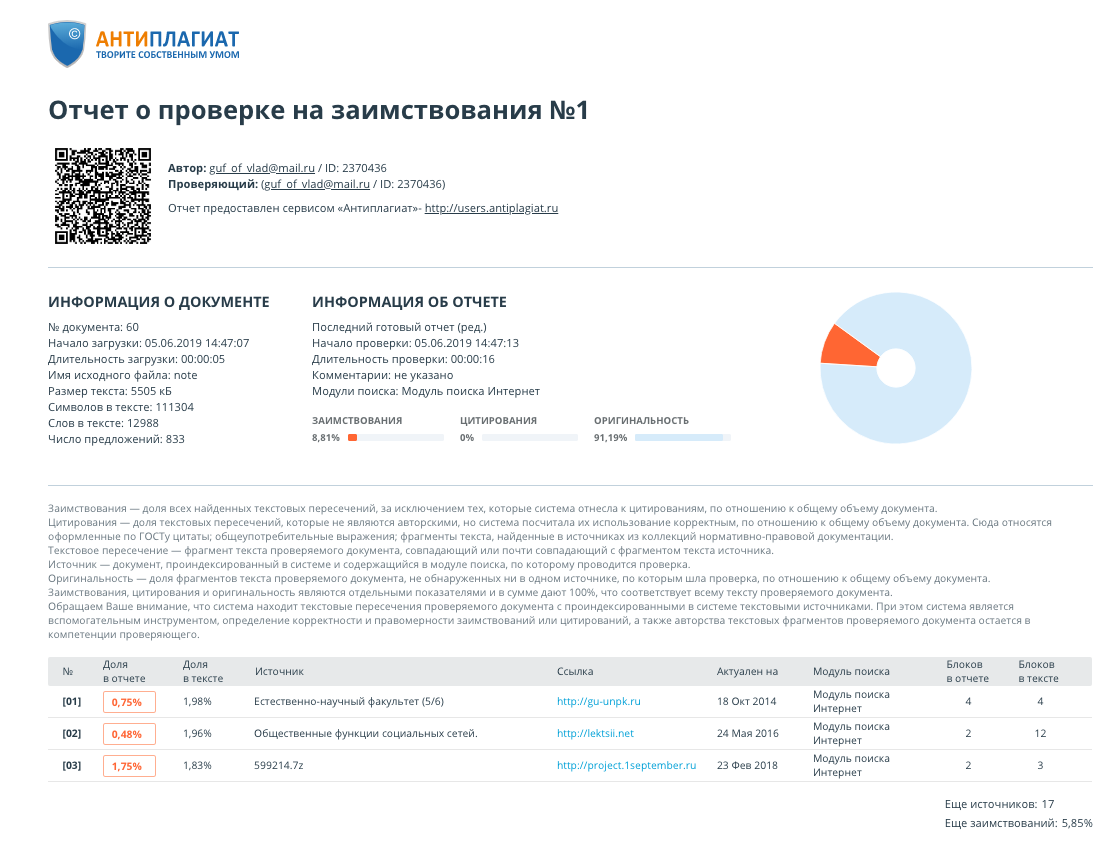
\includegraphics[scale=0.42]{antiplagiat.png} 
    \end{figure}
    \vspace{-5mm}
      \centerline{Рисунок Б -- Отчет о проверке на заимствования}
    
    \newpage
  
  \begin{center}
  \textbf{
  \MakeUppercase{Приложение В}\\
  (справочное)\\
  Описание схемы базы данных}
  \end{center}
  \addcontentsline{toc}{section}{Приложение В (справочное) Описание схемы базы данных}
  
  \lstinputlisting[style=fsharpstyle]{appendices/db_schema.ndef}
  
  \newpage
  
  \begin{center}
  \textbf{
  \MakeUppercase{Приложение Г}\\
  (справочное)\\
  Конфигурационные файлы проекта}
  \end{center}
  \addcontentsline{toc}{section}{Приложение Г (справочное) Конфигурационные файлы проекта}
  
  \lstinputlisting[style=js]{appendices/.eslintrc}
  \newpage
  \lstinputlisting[style=js]{appendices/package.json}

\end{document}

% \includepdf позволяет включить в результирующий pdf документ часть другого pdf документа, сделанного
% например не с помощью TeX. Бывает полезно, если какие-то диаграммны нарисованы, например, с помощью 
% Microoft Office и сохранены в pdf.
%\includepdf[pages={-}]{documents_list.pdf}